\documentclass[12pt, twosides]{report}   	
\usepackage{import} 
\usepackage[utf8]{inputenc}
\usepackage{geometry} 
\usepackage{imakeidx}
 \geometry{
 a4paper,
 left=25mm,
 top=25mm,
 right=25mm,
 bottom=25mm
 }               						
\geometry{letterpaper}                   		
\usepackage{graphicx}
\usepackage{comment}				
\usepackage{amsmath}						
\usepackage{amssymb}
\usepackage{enumerate}
\usepackage[defaultlines=3, all]{nowidow}
\usepackage{courier}
\usepackage{float}
\usepackage{cite}
\usepackage{booktabs}
\usepackage{subcaption}
\usepackage{rotating}
\usepackage{fancyhdr}
\usepackage{slashed}
\usepackage{rotating}
\usepackage{hyperref}
\usepackage{tcolorbox}
\usepackage{titlesec}
\usepackage{menukeys}
\usepackage{tabularx}
\usepackage{longtable}
\usepackage{tikz}
\usetikzlibrary{shapes.geometric}
\usetikzlibrary{arrows}
 
\titleformat{\chapter}[display]
  {\normalfont\bfseries}{\Huge Chapter \thechapter}{0pt}{\Huge}

\usepackage[utf8]{inputenc}
\usepackage{listings}
\usepackage{color}

\definecolor{codegreen}{rgb}{0,0.6,0}
\definecolor{codegray}{rgb}{0.5,0.5,0.5}
\definecolor{codepurple}{rgb}{0.58,0,0.82}
\definecolor{backcolour}{rgb}{1, 1, 1} %{0.95,0.95,0.92}
\definecolor{orange}{RGB}{255,127,0}
\definecolor{purple}{RGB}{144,0,144}
\definecolor{grey}{RGB}{235,235,235}
\definecolor{mygrey}{RGB}{235,235,255}
\definecolor{myblue}{RGB}{0,102,255}
\definecolor{myred}{RGB}{221,50,50}
\definecolor{mygreen}{RGB}{0,170,0}
\definecolor{myGrey}{RGB}{169,169,169}
\definecolor{myblack}{RGB}{0,0,0}
\definecolor{paleblue}{RGB}{158,214,255}
\definecolor{paleyellow}{RGB}{255,216,0}

\newcommand*{\pybullet}{
	\item[{\includegraphics[width=0.3cm]{Pictures/pythonsym.png}}]}

% Author Identifications
\newcommand{\will}[1]{{\color{purple}{#1}}}
\newcommand{\reese}[1]{{\color{red}{#1}}}
\newcommand{\david}[1]{{\color{magenta}{#1}}}
\newcommand{\aran}[1]{{\color{blue}{#1}}}

\makeatletter
\newcommand{\chapterauthor}[1]{%
  {\parindent0pt\vspace*{-25pt}%
  \linespread{1.1}\large\scshape#1%
  \par\nobreak\vspace*{35pt}}
  \@afterheading%
}
\makeatother
% Header and Footer formatting
\pagestyle{fancy}
% Added by David to remove the Chapter N. that was present in the headers
\renewcommand{\chaptermark}[1]{\markboth{\space#1}{}}
\fancyhf{}
% Added by David to include author last names
% \fancyhead[l]{Roper, Wilkinson, Turner, Hubbard, Romer, Loveday} 
\fancyhead[l]{PIP Python Lab Book} 
\fancyfoot[c]{\thepage}

\tikzset{
startend/.style = {draw,fill=red, circle},
operation/.style = {rectangle, draw,fill=paleblue,line width=0.04cm, text width=3.5em, text centered, minimum height=2.5em,rounded corners},
question/.style = {diamond, draw,fill=paleyellow,line width=0.04cm, minimum height=1em, minimum width=8em, text width=7em, text centered, inner sep=0pt},
line/.style = {draw,line width=0.05cm,rounded corners, -latex'},
coord/.style={coordinate}
}

\newcommand{\lfill}{\underline{\hspace*{0.8cm}}}
\newcommand{\linespan}{\begin{center}\rule{14cm}{0.4pt}\end{center}}

% Automatic centering of all figures
\makeatletter
\g@addto@macro\@floatboxreset\centering
\makeatother

% Code listing environments
\lstdefinestyle{mystyle}{
    language=C++,
    backgroundcolor=\color{grey},   
    commentstyle=\color{codegreen},
    keywordstyle=\color{magenta},
    numberstyle=\tiny\color{codegray},
    stringstyle=\color{codepurple},
    basicstyle=\footnotesize,
    breakatwhitespace=false,         
    breaklines=true,                 
    captionpos=b,                    
    keepspaces=true,                 
    numbersep=5pt,                  
    showspaces=false,                
    showstringspaces=false,
    showtabs=false,                  
    tabsize=2
}

% What follows here is a python language definition I found on stackoverflow and have been adapting (will)
\usepackage{xcolor}
\definecolor{maroon}{cmyk}{0, 0.87, 0.68, 0.32}
\definecolor{halfgray}{gray}{0.55}
\definecolor{ipython_frame}{RGB}{207, 207, 207}
\definecolor{ipython_bg}{RGB}{247, 247, 247}
\definecolor{ipython_red}{RGB}{186, 33, 33}
\definecolor{ipython_green}{RGB}{0, 128, 0}
\definecolor{ipython_lightgreen}{RGB}{0, 220, 0}
\definecolor{ipython_cyan}{RGB}{64, 128, 128}
\definecolor{ipython_purple}{RGB}{170, 34, 255}

\lstset{
    breaklines=true,
    %
    extendedchars=true,
    literate=
    {á}{{\'a}}1 {é}{{\'e}}1 {í}{{\'i}}1 {ó}{{\'o}}1 {ú}{{\'u}}1
    {Á}{{\'A}}1 {É}{{\'E}}1 {Í}{{\'I}}1 {Ó}{{\'O}}1 {Ú}{{\'U}}1
    {à}{{\`a}}1 {è}{{\`e}}1 {ì}{{\`i}}1 {ò}{{\`o}}1 {ù}{{\`u}}1
    {À}{{\`A}}1 {È}{{\'E}}1 {Ì}{{\`I}}1 {Ò}{{\`O}}1 {Ù}{{\`U}}1
    {ä}{{\"a}}1 {ë}{{\"e}}1 {ï}{{\"i}}1 {ö}{{\"o}}1 {ü}{{\"u}}1
    {Ä}{{\"A}}1 {Ë}{{\"E}}1 {Ï}{{\"I}}1 {Ö}{{\"O}}1 {Ü}{{\"U}}1
    {â}{{\^a}}1 {ê}{{\^e}}1 {î}{{\^i}}1 {ô}{{\^o}}1 {û}{{\^u}}1
    {Â}{{\^A}}1 {Ê}{{\^E}}1 {Î}{{\^I}}1 {Ô}{{\^O}}1 {Û}{{\^U}}1
    {œ}{{\oe}}1 {Œ}{{\OE}}1 {æ}{{\ae}}1 {Æ}{{\AE}}1 {ß}{{\ss}}1
    {ç}{{\c c}}1 {Ç}{{\c C}}1 {ø}{{\o}}1 {å}{{\r a}}1 {Å}{{\r A}}1
    {€}{{\EUR}}1 {£}{{\pounds}}1
}

%%
%% Python definition (c) 1998 Michael Weber
%% Additional definitions (2013) Alexis Dimitriadis
%% modified by me (should not have empty lines)
%%
\lstdefinelanguage{iPython}{
    morekeywords={access,and,break,class,continue,def,del,elif,else,except,exec,finally,for,from,global,if,import,in,is,lambda,not,or,pass,print,raise,return,try,while},%
    %
    % Built-ins
    morekeywords=[2]{abs,all,any,basestring,bin,bool,bytearray,callable,chr,classmethod,cmp,compile,complex,delattr,dict,dir,divmod,enumerate,eval,execfile,file,filter,float,format,frozenset,getattr,globals,hasattr,hash,help,hex,id,input,int,isinstance,issubclass,iter,len,list,locals,long,map,max,memoryview,min,next,object,oct,open,ord,pow,property,range,raw_input,reduce,reload,repr,reversed,round,set,setattr,slice,sorted,staticmethod,str,sum,super,tuple,type,unichr,unicode,vars,xrange,zip,apply,buffer,coerce,intern},%
    %
    sensitive=true,%
    morecomment=[l]\#,%
    morestring=[b]',%
    morestring=[b]",%
    %
    morestring=[s]{'''}{'''},% used for documentation text (mulitiline strings)
    morestring=[s]{"""}{"""},% added by Philipp Matthias Hahn
    %
    morestring=[s]{r'}{'},% `raw' strings
    morestring=[s]{r"}{"},%
    morestring=[s]{r'''}{'''},%
    morestring=[s]{r"""}{"""},%
    morestring=[s]{u'}{'},% unicode strings
    morestring=[s]{u"}{"},%
    morestring=[s]{u'''}{'''},%
    morestring=[s]{u"""}{"""},%
    %
    % {replace}{replacement}{lenght of replace}
    % *{-}{-}{1} will not replace in comments and so on
    literate=
    {á}{{\'a}}1 {é}{{\'e}}1 {í}{{\'i}}1 {ó}{{\'o}}1 {ú}{{\'u}}1
    {Á}{{\'A}}1 {É}{{\'E}}1 {Í}{{\'I}}1 {Ó}{{\'O}}1 {Ú}{{\'U}}1
    {à}{{\`a}}1 {è}{{\`e}}1 {ì}{{\`i}}1 {ò}{{\`o}}1 {ù}{{\`u}}1
    {À}{{\`A}}1 {È}{{\'E}}1 {Ì}{{\`I}}1 {Ò}{{\`O}}1 {Ù}{{\`U}}1
    {ä}{{\"a}}1 {ë}{{\"e}}1 {ï}{{\"i}}1 {ö}{{\"o}}1 {ü}{{\"u}}1
    {Ä}{{\"A}}1 {Ë}{{\"E}}1 {Ï}{{\"I}}1 {Ö}{{\"O}}1 {Ü}{{\"U}}1
    {â}{{\^a}}1 {ê}{{\^e}}1 {î}{{\^i}}1 {ô}{{\^o}}1 {û}{{\^u}}1
    {Â}{{\^A}}1 {Ê}{{\^E}}1 {Î}{{\^I}}1 {Ô}{{\^O}}1 {Û}{{\^U}}1
    {œ}{{\oe}}1 {Œ}{{\OE}}1 {æ}{{\ae}}1 {Æ}{{\AE}}1 {ß}{{\ss}}1
    {ç}{{\c c}}1 {Ç}{{\c C}}1 {ø}{{\o}}1 {å}{{\r a}}1 {Å}{{\r A}}1
    {€}{{\EUR}}1 {£}{{\pounds}}1,
    %
    literate=
    *{-}{{{\color{ipython_purple}$-$}}}1
     {?}{{{\color{ipython_purple}?}}}1
     {^}{{{\color{ipython_purple}\^{}}}}1
     {=}{{{\color{ipython_purple}\texttt{\textbf{=}}}}}1
     {+}{{{\color{ipython_purple}$+$}}}1
     {*}{{{\color{ipython_purple}$\ast$}}}1
     {/}{{{\color{ipython_purple}$/$}}}1
     {+=}{{{\color{ipython_purple}+\texttt{\textbf{=}}}}}1
     {-=}{{{\color{ipython_purple}-\texttt{\textbf{=}}}}}1
     {*=}{{{\color{ipython_purple}$\ast$\texttt{\textbf{=}}}}}1
     {/=}{{{\color{ipython_purple}/\texttt{\textbf{=}}}}}1
     {>}{{{\color{ipython_purple}$\boldsymbol{>}$}}}1
     {<}{{{\color{ipython_purple}$\boldsymbol{<}$}}}1
     { == }{{{\color{ipython_purple}~\texttt{\textbf{=}}\,\texttt{\textbf{=}}~}}}4
     { <= }{{{\color{ipython_purple}~$\boldsymbol{<}$\,\texttt{\textbf{=}}~}}}4
     { >= }{{{\color{ipython_purple}~$\boldsymbol{>}$\,\texttt{\textbf{=}}~}}}4
    %  {0}{{\color{ipython_green}{0\color{black}}}}1
    %  {1}{{\color{ipython_green}{1\color{black}}}}1
    %  {2}{{\color{ipython_green}{2\color{black}}}}1
    %  {3}{{\color{ipython_green}{3\color{black}}}}1
    %  {4}{{\color{ipython_green}{4\color{black}}}}1
    %  {5}{{\color{ipython_green}{5\color{black}}}}1
    %  {6}{{\color{ipython_green}{6\color{black}}}}1
    %  {7}{{\color{ipython_green}{7\color{black}}}}1
    %  {8}{{\color{ipython_green}{8\color{black}}}}1
    %  {9}{{\color{ipython_green}{9\color{black}}}}1
    %  {.0}{{\color{ipython_green}{.0\color{black}}}}1
     {-1}{{\color{black}{-1}}}1
     {-2}{{\color{black}{-2}}}1
     {-3}{{\color{black}{-3}}}1
     {-4}{{\color{black}{-4}}}1
     {-5}{{\color{black}{-5}}}1
     {-6}{{\color{black}{-6}}}1
     {-7}{{\color{black}{-7}}}1
     {-8}{{\color{black}{-8}}}1
     {-9}{{\color{black}{-9}}}1
    %  {j}{{\color{ipython_green}\textbf{j}}}1
    %  {)}{{\color{ipython_lightgreen}{)}}}1 
    %  {(}{{\color{ipython_lightgreen}{(}}}1
    %  {]}{{\color{ipython_lightgreen}{]}}}1 
    %  {[}{{\color{ipython_lightgreen}{[}}}1
    ,
    %
    identifierstyle=\color{black}\ttfamily,
    commentstyle=\color{ipython_cyan}\ttfamily,
    stringstyle=\color{ipython_red}\ttfamily,
    keepspaces=true,
    showspaces=false,
    showstringspaces=false,
    %
    rulecolor=\color{ipython_frame},
    frame=single,
    frameround={t}{t}{t}{t},
    %framexleftmargin=6mm,
    %numbers=left,
    %numberstyle=\scriptsize\color{halfgray},
    %
    %
    backgroundcolor=\color{ipython_bg},
    %   extendedchars=true,
    basicstyle=\footnotesize\color{black},
    keywordstyle=\color{ipython_green}\ttfamily,
}

\lstdefinestyle{PY}{
    language=iPython,
    backgroundcolor=\color{grey},
    keywordstyle=\bfseries\color{ipython_green},
    commentstyle=\bfseries\color{myGrey},
    identifierstyle=\color{myblack},
    stringstyle=\bfseries\color{myred},
    emph={int,bool,type,None,len,range,input,1,2,3,4,5,6,7,8,9},
    emphstyle=\color{ipython_green}\textbf,
    showstringspaces=false,
    rulecolor=\color{black},
    breaklines=true,
    postbreak=\mbox{\textcolor{red}{$\hookrightarrow$}\space}
}
%added by Reese to prevent syntax highlighting in jupyter outputs
\lstdefinestyle{PY_out}{
    language=iPython,
    backgroundcolor=\color{white},
    keywordstyle=\color{myblack},
    commentstyle=\color{myblack},
    identifierstyle=\color{myblack},
    stringstyle=\color{myblack},
    emph={int,bool,type,None,len,range,input,1,2,3,4,5,6,7,8,9},
    emphstyle=\color{myblack},
    showstringspaces=false,
    rulecolor=\color{black},
    breaklines=true,
    postbreak=\mbox{\textcolor{red}{$\hookrightarrow$}\space}
}


\begin{document}
\begin{titlepage}
\begin{center}

%\vspace*{2cm} % adjust as you wish
        
  {\Huge\textbf{PIP Python Lab Book}}
  \vspace{0.5cm} % adjust as you wish

{\Large University of Sussex}
\vspace{1cm} % adjust as you wish
      

{\large W. Roper; R. Wilkinson; D. J. Turner; M. Hubbard; A.K Romer; J. Loveday\\

Course Convener: Dr Jon Loveday\\
        
Last Update: \today\\
        
}

\vspace{2cm} % adjust as you wish

\includegraphics[width=0.8\linewidth]{Pictures/pythonxkcd.png}\\

\end{center}
\end{titlepage}

%\maketitle
\pagenumbering{roman}

%\addcontentsline{toc}{section}{Preface}
%\section*{Individual Work}

Reese, David and I (Will) need to port and edit what exists for chapters 1-5, as these already function as a good introduction to python (with a greater emphasis on functions and maybe change up some examples/exercises). We also need to make sure the exercises and assignments work in Jupyter.

I will edit this as time goes on. Anything below in black is part of the main module, \color{blue} blue \color{black} corresponds to the advanced chapters and \color{red} red \color{black} corresponds to the `Nerd Glossary' (mini descriptions not corresponding to entire chapters).

\subsection*{Will}

\begin{itemize}
	
\pybullet \texttt{numpy} and \texttt{scipy} (chapters 8 and 9).
\pybullet \color{blue}Scientific Computing linking chapter (post chapter 9).\color{black}
\pybullet \color{blue}Dictionaries and Sets.\color{black}
\pybullet \color{red} Data formats (HDF5, text, csv, FITS etc). \color{black}
	
\end{itemize}

\subsection*{Reese}

\begin{itemize}
	
\pybullet Convert from using \texttt{csv} to use \texttt{pandas} (chapter 5).
\pybullet \color{blue}Object orientated \texttt{python} (with help from Will??). \color{black}
	
\end{itemize}

\subsection*{David}

\begin{itemize}
	
\pybullet \color{blue}Fancy \texttt{matplotlib}.\color{black}
	
\end{itemize}

\subsection*{Aran}

\begin{itemize}
	
\pybullet \color{blue}Intro to C++.
\pybullet \LaTeX\ chapter including \texttt{BibTex}, \texttt{Zotero} and \texttt{Mendeley}. \color{black}
\pybullet \color{red}\texttt{ROOT}. \color{black}
	
\end{itemize}

\subsection*{Authorless or multi-author}

\begin{itemize}
	
\pybullet \color{blue}HTML (David or Reese?).
\pybullet UNIX (shell, etc).\color{black}
\pybullet \color{red} PEP 8. \color{black}
\pybullet \color{red} Brief breakdown of different IDEs (Atom -Reese, PyCharm, Spyder etc). \color{black}
\pybullet \color{red} Working with command line editors (nano, vim, emacs etc). \color{black}
\pybullet \color{red} \texttt{SeXtractor}. \color{black}
\pybullet \color{red}\texttt{XSPEC}. \color{black}
\pybullet \color{red} \texttt{julia}. \color{black} (we should just refer to the Julia course (which is free))
\pybullet \color{red} \texttt{astropy} with particular focus on how awesome \texttt{.units} and \texttt{.constants} are! \color{black}
\pybullet \color{red} `Nice' HPC use. \color{black} (Reese from Roberto comments/peeves)
\pybullet \color{red} Simple Parallisation? \color{black}
	
\end{itemize}

\newpage

\section*{General}

\begin{enumerate}
    \item Fix formatting for chapter authors.
    \item Edit authors actually involved in each chapter when known.
    \item Make sure all examples are PEP8 compliant.
\end{enumerate}

\section*{Chapter 1}

\noindent Old outcomes:
\begin{enumerate} 
\item Generate a simple flow chart.
\item Run Python on the University computers using the {\bf Jupyter} interface.
\item Interrupt a (pseudo) infinite loop.
\item Use the {\tt print} command.
\item Use Python as a simple calculator.
\item Use three different Python data types: integer, float, and complex.
\item Add comments to your Python codes.
\end{enumerate}

\noindent Things to add/change:
\begin{enumerate}
    \item Never too much emphasis on good commenting, otherwise this is a mostly good intro as it stands.
    \item Add flow chart example.
    \item Exit Verbatim.
    \item Generally clean up formatting due to porting.
    \item Change iPython ouput to jupyter style.
\end{enumerate}

\section*{Chapter 2}

\noindent Old outcomes:
\begin{enumerate}
\item still do everything described in the script for Lab Session 1,
\item add comments to your scripts,
\item manipulate strings,
\item use boolean's,
\item use tuples and lists,
\item use the {\tt input} command,
\item use indentation and colons.
\end{enumerate}

\noindent Things to add/change:

\section*{Chapter 3}

\noindent Old outcomes:
\begin{enumerate}
\item understand the use of tab indents and colons,
\item use {\tt if}, {\tt while}, {\tt for} statements,
\item use loops,
\item write basic codes,
\item use the modulo (\%) operator,
\item use the {\tt range} function,
\item use and define your own {\bf functions},
\item use the {\tt lambda} statement (optional),
\item use the dictionary data type (optional).
\end{enumerate}

\noindent Things to add/change:

\section*{Chapter 5}

\noindent Old outcomes:
\begin{enumerate}
\item Know what Python modules are and what they are for. 
\item Know how to load Python modules.
\item Know how to find out what functions are inside a given module and how to get help with those functions.
\item Be familiar with the {\tt pylab} module (including the {\tt arange} function).
\item Be familiar with the the {\tt random} module.
\item Be able to make basic level plots.
\end{enumerate}

\noindent Things to add/change:
\begin{enumerate}
    \item Obliterate any reference to pylab with as much fire as it takes.
\end{enumerate}

\section*{Chapter 6}

\noindent Old outcomes:
\begin{enumerate}
\item Be familiar with the the {\tt csv} module.
\item Be able to make intermediate level plots (including adding error bars).
\item Be able to carry out basic fitting of data to models.
\end{enumerate}

\noindent Things to add/change:

\begin{enumerate}
    \item Switch to pandas.
\end{enumerate}

\section*{Chapter 8}

\noindent Old outcomes:
\begin{enumerate}
\item Be able to make n-dimensional arrays
\item Be able to manipulate vectors and n-dimensional arrays
\item Be able to carry out matrix and vector calculations
\item Be able to plot arrays (i.e. 2D shapes).
\end{enumerate}

\noindent Things to add/change:

\section*{Chapter 9}

\noindent Old outcomes:
\begin{enumerate}
\item Be able to save image and text files.
\item Be able to make histograms with Python.
\item Be able to generate simple webpages with HTML and Python.
\end{enumerate}

\noindent Things to add/change:

\section*{Glossary}

\noindent Need to:
\begin{enumerate}
    \item Change formatting to listings.
    \item Generally fix all the latex bugs...
    \item Add anything now relevant given new module.
    \item Check Python 3 compatibility.
\end{enumerate}

\section*{Work Done/Changelog}

Update here when you have done something so pay can be attributed properly.

\subsection*{Chapter 1}

\begin{itemize}
    \pybullet \will{Ported from old version.}
    \pybullet \will{Minor bug fixing.}
    \pybullet \will{Converted all examples to lstlisting PY environments.}
    \pybullet \will{Removed incorrect python-2 text.}
    \pybullet \will{Added a section on commenting to introduce it as early as possible.}
    \pybullet \will{Added some advanced red boxes.}
\end{itemize}

\subsection*{Chapter 2}

\begin{itemize}
    \pybullet \will{Ported from old version.}
    \pybullet \will{Minor bug fixing.}
    \pybullet \will{Converted all examples to lstlisting PY environments.}
    \pybullet \will{Removed commenting subsection since now in Chapter 1.}
    \pybullet \will{Added stackoverflow.com to the preamble.}
    \pybullet \will{Added advanced section on the is keyword and moved the copy stuff to within it}
\end{itemize}

\subsection*{Chapter 3}

\begin{itemize}
    \pybullet \will{Ported from old version.}
    \pybullet \will{Minor bug fixing.}
    \pybullet \will{Converted all examples to lstlisting PY environments.}
    \pybullet \will{Converted to python 3 where necessary.}
    \pybullet \will{Added extra context around examples.}
    \pybullet \will{Made dictionary a proper section rather than optional.}
\end{itemize}

\subsection*{Chapter 4}

\begin{itemize}
    \pybullet 
\end{itemize}

\subsection*{Chapter 5}

\begin{itemize}
    \pybullet \will{Ported from old version.}
    \pybullet \will{Minor bug fixing.}
\end{itemize}

\subsection*{Chapter 6}

\begin{itemize}
    \pybullet 
\end{itemize}

\subsection*{Chapter 7}

\begin{itemize}
    \pybullet 
\end{itemize}

\subsection*{Chapter 8}

\begin{itemize}
    \pybullet 
\end{itemize}

\subsection*{Chapter 9}

\begin{itemize}
    \pybullet 
\end{itemize}

\subsection*{Chapter 10}

\begin{itemize}
    \pybullet 
\end{itemize}

\subsection*{Chapter 11}

\begin{itemize}
    \pybullet 
\end{itemize}

\subsection*{Introduction to C$++$}

\begin{itemize}
    \pybullet \aran{First draft written and encorporated.}
\end{itemize}

\subsection*{Nerd Glossary}

\begin{itemize}
    \pybullet 
\end{itemize}


%\newpage

\newpage
\clearpage
\fancyhead[r]{\leftmark}
\tableofcontents

\clearpage

\chapter{Introduction}
% \chapterauthor{W. Roper; R. Wilkinson; D. J. Turner; A. K. Romer; M. Hubbard;}
\section*{Preamble}
The \texttt{Python} programming language is ubiquitous in science, especially in Physics. It is an extremely powerful tool which can be utilised for everything from making simple games to simulating the evolution of the Universe. In fact, `Big Tech' companies such as Google and Facebook use \texttt{Python} behind the scenes of many services you use daily. 

Whether or not you have programmed before this module will give you the tools you need to perform research, complete assignments and most importantly will give you marketable skills that can help you get a job after your degree. If you're anything like the authors of this document it will also have the unintended consequence of giving you an \textbf{unhealthy coding addiction}, which will be impossible to kick.

\section*{Module Structure}

This module is run in tandem with Physics In Practice (PIP) but don't be fooled, it is just as important as many of the full fat modules you'll do in your degree. As such, it is structured in much the same way as your other modules with teaching, assignments, and exercises within the lab book. The main difference is in \textbf{how} the material is taught; rather than traditional lectures you'll take part in lab sessions and work through this document chapter by chapter. These lab sessions, starting with a very short introductory talk, will give you direct contact with the AT and the lecturers to help you with any problems.
% In the light of the current situation this is not the case and instead we will be running three/four hour long sessions a week via zoom in which at least 1 of us, if not more will be present to offer help and explain concepts.

In addition to these sessions we will record and upload any relevant short lectures as videos to canvas to be digested at anytime. We also would like to draw your attention to the discussions tab on canvas, here you can post questions and one of us will get back to you as soon as we can or we can plan a full explanation for one of the workshops.

Each chapter in this document is typically a single lab session; this translates to a single chapter per week. The exceptions to this rule are weeks 4, 7, and 10 in which you will have an opportunity to work on assignments.
The first (week 4) assignment is formative and will be peer marked.
We will give you further details on this marking in the introduction sessions.
The second two assignments will be tutor marked and contribute equally to the
portfolio mark, worth 30\% of the PIP module mark.
% there will be competency tests. These competency tests enable us to gauge how everyone is progressing in a formative manner and will also lead to a competency certificate for you, showing proof of your capabilities. They will be peer marked and the results entered through a link that will be provided on canvas. 

We will repeat this again and again: do not take the low weighting of this sub-module as a reflection of it's importance, \texttt{Python} is an essential skill. Failure to engage now \textbf{will} lead to troubles down the road when the weightings are far higher and contributory. We have seen it before and, sadly, will undoubtedly see it again where a student hits a \textbf{Python} related problem in a later module which was discussed during this module. 

\section*{Lab book}
You will find the entirety of this lab book uploaded to canvas (any updates to the content will be uploaded when necessary) in case you wish to move through the course faster than planned. However, not everyone enjoys coding as much as we do, \textbf{so do not worry if you find yourself struggling a little}, please make sure to ask the lecturers or AT for help if you need it. Programming can be daunting for the uninitiated and it can take time to start thinking like a programmer, but when you do your increased understanding of logic will help you throughout your whole degree/life.

Each chapter will begin with a list of learning outcomes for that section followed by the content containing some worked examples. At the end of each section, there will be some exercises for you to complete to check your understanding of the chapter (remember to ask the ATs for help if you're stuck, they will \textbf{likely} have made all the same mistakes).

\begin{tcolorbox}[colback=red!5!white,colframe=red!75!black]

Throughout this lab book you will find boxes like this. These contain information which is beyond the scope of this module but will be important should you decide to continue into computationally heavy research or a career using \texttt{Python}. They will be useful for future reference, or are just interesting, but don't be intimidated if you don't immediately understand the content contained within them.
	
\end{tcolorbox}

%After the main body of the lab book you will find chapters that take a look at some more advances features of \texttt{Python} and scientific computing as a whole. Following the advanced chapters is an affectionately named `Nerd's Glossary', containing small sections detailing niche concepts which we have deemed `interesting' and useful for reference in the future. Should you come up with anything we've omitted that you think should be included, do let us know.

\section*{Assignments}
There will be three assignments, the first of which is unweighted and will be peer marked, and they will be marked on:

\begin{itemize}
    \item The final answers you have.
    \item Coding style (including comments!!! More on this in Chap.\ref{chap:jupyter}).
    \item How logical and efficient your approach is.
\end{itemize}

\noindent The assignments will be uploaded to Canvas and should be submitted by the deadlines in weeks 4, 7 and 10. These assignments, like all others, should be completed and submitted on your own, containing only your own work (a reminder about collusion and plagiarism is provided in section \ref{subsec:collusion}). % These assignments are in addition to the competency tests.

\section*{Cautionary Note}

This module has been redesigned to use \texttt{Python-3}. This is the newest version of  \texttt{Python} (replacing \texttt{Python-2}) and the version that's installed on the University system. You may come across instances of \texttt{Python-2} throughout your degree (and beyond) since it is still widely used but official support has now ended. There is little difference between the two versions on the surface, so don't worry about this too much. The main differences are the syntax of the \texttt{print} function and how the code behaves when dividing one integer by another.

\begin{tcolorbox}[colback=red!5!white,colframe=red!75!black]
The \texttt{print} function (as you may have guessed), prints a value to the screen.
Should you be interested, the exact differences between the \texttt{print} function and integer division in each  \texttt{Python} version are as follows:

\noindent\textbf{Python-2}
\begin{lstlisting}[style=PY]
In [1]: print 'Hello World'  # print statement, notice the lack of ()
        1 / 2  # integer division
        1.0 / 2.0  # float division
\end{lstlisting}
\begin{lstlisting}[style=PY, backgroundcolor=\color{white}]
Out[1]: 'Hello World'
        0  # 0 since 1 is not divisible by 2
        0.5  # float division gives the expected result of a half
\end{lstlisting}

\noindent\textbf{Python-3}
\begin{lstlisting}[style=PY]
In [2]: print('Hello World')  # print function, notice the parentheses
        1 / 2  # float division is automatically assumed in\texttt{Python-3}
        1 // 2  # integer division now has a different operator
\end{lstlisting}
\begin{lstlisting}[style=PY, backgroundcolor=\color{white}]
Out[2]: 'Hello World'
        0.5  # float division
        0  # integer division
\end{lstlisting}
\end{tcolorbox}





\chapter{Some Useful Terminology}
This is intended to be a quick point of reference for any terminology that appears in the script that may need clarification. Please feel free to suggest additions! This will evolve over time to contain anything and everything useful.

\begingroup
\setlength{\tabcolsep}{10pt} % Default value: 6pt
\renewcommand{\arraystretch}{1.5} % Default value: 1
% \begin{table}[H]
% \begin{center}
\begin{longtable}{l p{12cm}}
%\multicolumn{2}{|c|}{\textbf{General Use:}}\\\hline
Data & This can be anything: a number, a set of numbers, a character, a set of characters, an image etc. Essentially any outside input you want to handle with \texttt{Python} could be called "data". \\
Data type & The variety of a particular data, kind of self explanatory but here for completeness. \\
Data structure & Any container for data. Think of a table or list in the real world, this is where you put \textit{things}. In simple terms a "structure" in which you store "data". \\
Variable & These are labels that you store things in. Not to be confused with a data structure, a variable essentially labels a value, a data structure or an object and allows the computer to store and use what you have labelled. They are much like variables in maths, $m$ representing a mass, $F$ representing a force, $c$ representing the fundamental speed of light. What the computer actually does is link the label (variable) to a memory address at which your value/object is stored. \\
Comment & A statement within a piece of code not executed by the computer but instead included to provide context to a human reader of the code. \\
Function & A reusable segment of code defined by the programmer which contains a set of operations, taking in values and returning the results after execution of the commands within the function. \\
Argument & A value that is passed into a function to be used inside the function. These can be anything your function needs to operate. Also often called a parameter but rarely in \texttt{Python}. \\
Module & Simply, a module is a file consisting of \texttt{Python} code which can be loaded in your \texttt{Python} programs to add functionality not native to \texttt{Python}. \\
PEP-8 & This is a set of guidelines for writing good ``Pythonic'' code which makes it easier to read other peoples code. \\
IDE & (Integrated Development Environments) A piece of software that provides everything a user needs to write code; think Word but for code development. \\
Keyword & Keywords are the reserved words in \texttt{Python} used to perform specific operations. We cannot use a keyword as a variable name, function name or any other identifier as this would overwrite the python native behaviour of the word. \\
\caption {Some useful terminology for the module.} . \\
\end{longtable}
% \end{center}
% \end{table}
\endgroup


\chapter{Jupyter: Quick reference}
\section*{Jupyter Keyboard Shortcuts}
\label{JupKeyShort}

This section is meant to act as a quick reference for the most useful shortcuts in \texttt{jupyter}, it'll become more useful when you've become more familiar with the software. It is worth trying to remember these shortcuts, as they can greatly improve the speed of workflow, and are just generally more convenient.

\begin{table}[H]
\begin{center}
\begin{tabular}{|l | p{5.5cm}|}
\hline
\multicolumn{2}{|c|}{\textbf{General Use:}}\\\hline
\texttt{\keys{shift+enter}} & Run Current Cell\\\hline
\texttt{\keys{alt+enter}} & Run and insert new cell below\\\hline
\texttt{\keys{ctrl+S}} & Save Notebook\\\hline
\multicolumn{2}{|c|}{\textbf{Command mode shortcuts:}}\\\hline
\texttt{\keys{esc+B}} & Insert cell below\\\hline
\texttt{\keys{esc+A}} & Insert cell above\\\hline
\texttt{\keys{esc+D,D}} & Delete current cell\\\hline
\texttt{\keys{esc+\arrowkeyup}} & Go to the cell above\\\hline
\texttt{\keys{esc+\arrowkeydown}} & Go to the cell below\\\hline
\texttt{\keys{esc+C}} & Copy the current cell\\\hline
\texttt{\keys{esc+X}} & Cut the current cell\\\hline
\texttt{\keys{esc+V}} & Paste cell\\\hline
\multicolumn{2}{|c|}{\textbf{Cell editing shortcuts:}}\\\hline
\texttt{\keys{tab}} & Indent or code completion\\\hline
\texttt{\keys{ctrl+A}} & Select everything in a cell\\\hline
\texttt{\keys{ctrl+?}} & Comment out the current line\\\hline
\end{tabular}
\end{center}
\caption {Some of the most useful \texttt{jupyter} keyboard shortcuts.}
\end{table}

\pagenumbering{arabic}
\chapter{The Basics}
%\chapterauthor{PRATS}
\label{chap:jupyter}
\section{Learning Outcomes} 
\label{W1LO}

\noindent By the end of today's session you will know how to:
\begin{enumerate} 
\item Generate a simple flow chart, to understand their use in logic problems.
\item Run \texttt{Python} on the university computers using the \texttt{jupyter} interface.
\item Interrupt a (pseudo) infinite loop.
\item Use the {\tt print} function.
\item Use \texttt{Python} as a simple calculator.
\item Use three different \texttt{Python} data types: integer, float, and complex.
\item Add comments to your \texttt{Python} codes.
\end{enumerate}

\section{Preamble} 
\label{sec:preamle1}

We'll start slowly to make sure everyone feels confident with the absolute basics. We'll start by showing you how to get started using \texttt{jupyter}, a web browser application that is one of several ways of coding in \texttt{Python}.

You will then work through some simple calculations and work with data types and variables. You are free to move on to future chapters if you complete this quickly or already have an understanding of \texttt{Python} programming.

Lets start by making a flow chart to describe the following:

Something that includes a series of steps that you do so often that it is second nature (don't be rude/personal/gross! Shouldn't need saying but past experiences...), e.g. making a cup of tea, having a shower, getting the bus to campus.....

These flowcharts should be done by hand initially, but if you are keen and want to learn a new skill, you could try making them using online flowchart software such as {\tt lucidchart.com} or {\tt gliffy.com} or {\tt drawio.com}. Please note that not all of these packages work on Edge/Internet Explorer (try Chrome instead). These flow charts do not have anything with Jupyter. The intention is to get you thinking about how programming works, not to get you to write a code.

Each year we are asked "Why are we doing flowcharts?". So here is the answer: To fully understand the operations of a program, flowcharts are indispensable tools. In simple terms, programs operate by stepping through a set of instructions/decisions (the code) and executing them one at a time (just as you step through a flowchart). Although the examples above are simple, programs can get very complicated (astronomical survey analysis, data reduction at CERN, cosmological simulations). You can have tens of thousands of lines of code with multiple paths for data, a structure too complicated to just keep in your head. Flowcharts give a schematic view of the different paths data can take through these programs, and the possible decisions based on that data. Flowcharts get you to think about \textbf{how a program functions} before you've even written it, and are \textbf{an important skill} you may need later in your career. 

Simple example flow charts can be found in the appendix of one of this document's author's published papers (\href{https://arxiv.org/abs/2003.01187}{Roper et al. 2020}), mentioned here just to drive home that they are useful!

%\begin{tcolorbox}[colback=red!5!white,colframe=red!75!black]
\section{Running \texttt{Python} on the University computers}
\label{StartingPython}

\subsection{Running \texttt{Anaconda} for the first time}

The first time you use Anaconda on a University PC, you need to launch Anaconda via the Software Hub.
To do this, type 'software hub' into the search box at the bottom left of the screen, and run the {\em Software Hub} app, see Figure~\ref{fig:software_hub}:

\begin{figure}[htbp]  
\centering
\includegraphics[width=12cm]{Figures/software_hub.png}
\caption{Running Software Hub (first use of Anaconda).}
\label{fig:software_hub}
\end{figure}

Type anaconda into the software hub search box and click Launch
(Fig.~\ref{fig:anaconda_launch}).

\begin{figure}[htbp]  
\centering
\includegraphics[width=12cm]{Figures/anaconda_launch.png}
\caption{Launching Anaconda (first use).}
\label{fig:anaconda_launch}
\end{figure}

\subsection{Running \texttt{Anaconda} in subsequent sessions}

On subsequent use, you should only need to select Anaconda from the Windows {\tt Start} menu, see Fig.~\ref{fig:programmen}.

\begin{figure}[htbp]  
\centering
\includegraphics[width=7cm]{Figures/Capture2.PNG}
\includegraphics[width=7cm]{Figures/Capture2.PNG}
\caption{Running Anaconda, subsequent use.
  The program menu can be found in the bottom left corner}
\label{fig:programmen}
\end{figure}

\subsection{Running Jupyter Notebook}

After a few moments, the Anaconda Navigator will appear.  From it, launch Jupyter Notebook (Fig.~\ref{fig:jupyter_launch}).

\begin{figure}[htbp]  
\centering
\includegraphics[width=12cm]{Figures/jupyter_launch.png}
\caption{Launching Jupyter.}
\label{fig:jupyter_launch}
\end{figure}

{\bf Important}: any Jupyter notebooks you create should be stored under the folder {\tt OneDrive - University of Sussex}, otherwise they will only be saved on the particular PC that you are using.
Open the {\tt OneDrive - University of Sussex} folder and create a new sub-folder with a name such as \verb|PIP_Python|.
Open that sub-foldder and create a new Jupyter notebook using the {\tt New $\rightarrow$ Python 3} pull-down menu, see Figures~\ref{fig:onedrive} and \ref{fig:python_launch}.

\begin{figure}[htbp]  
\centering
\includegraphics[width=12cm]{Figures/onedrive.png}
\caption{Be sure to save notebooks under {\tt OneDrive - University of Sussex}.}
\label{fig:onedrive}
\end{figure}

\begin{figure}[htbp]  
\centering
\includegraphics[width=12cm]{Figures/python_launch.png}
\caption{Launching Python.}
\label{fig:python_launch}
\end{figure}

%% On the university machines you can start ``\textbf{jupyter notebook}'' via the Programs
%% Menu (Figure~\ref{programmen}) and the options under Anaconda (Figure~\ref{annaopt}).

%% \begin{figure}[H]  
%% \centering
%% \includegraphics[width=7cm]{Figures/Capture1.PNG}
%% \caption{The program menu can be found in the bottom left corner}
%% \label{programmen}
%% \end{figure}

%% \begin{figure}[H]  
%% \centering
%% \includegraphics[width=7cm]{Figures/Capture3.PNG}
%% \caption{How to find the \texttt{jupyter} Notebook option via the program menu.}
%% \label{annaopt}
%% \end{figure}

%% The Jupyter Notebook option starts a browser session and a few moments later a \texttt{jupyter} session will appear in your web browser. 
%% Also a console x-term window will pop up immediately (Figure~\ref{xterm}). {\bf Do not close the x-term window as this will stop your \texttt{jupyter} session from working.}  
%% %\end{tcolorbox}

%% %\begin{tcolorbox}[colback=red!5!white,colframe=red!75!black]

%% \begin{figure}[H]  
%% \centering
%% \includegraphics[width=14cm]{Figures/Capture4.PNG}
%% \caption{A \texttt{jupyter} notebook session with the x-term behind it.}
%% \label{xterm}
%% \end{figure}

%% You can now upload to that session an existing \texttt{jupyter} notebook file (extension .ipynb) or you make a new one (see Figure~\ref{OpenNew}).

%% \begin{figure}[H]  
%% \centering
%% \includegraphics[width=14cm]{Figures/OpenNew.png}
%% \caption{How to open a new \texttt{jupyter} notebook.}
%% \label{OpenNew}
%% \end{figure}

%% %\end{tcolorbox}

\section{Running \texttt{Python} on your own computer}

Throughout this term we will be using \texttt{jupyter notebooks}. \texttt{jupyter} is a web-browser application that allows you to create and share programs, which in our case will be written in \texttt{Python}. This section intends to help you install \texttt{Python} on you personal computer. Should you need to use \texttt{Python} on University computers rather than a personal computer the usual guide for this module can be found in Sec. \ref{StartingPython}. It is worth giving this a read anyway even if you are using a personal computer as it contains some important information.

The easiest way to setup everything you will need for the assessments and labs on your laptop or home PC, is by installing the \href{https://www.anaconda.com}{Anaconda software package} (\url{https://www.anaconda.com}). Anaconda is a `distribution' of \texttt{Python} that has several extra features that make it easier to improve \texttt{Python}'s capabilities; one of the most important is its package manager. 

When you reach chapter \ref{chap:modules}, you'll be introduced to \textbf{modules}, which are pieces of code that other people have written to expand \texttt{Python}'s capabilities. For instance, there are specialist modules for Astrophysics that make it easier for us to do common calculations and operations, such as loading in images from telescopes. \texttt{Python} has a built in way of installing new modules called \texttt{PIP}, but Anaconda adds a more sophisticated package manager which makes sure that all of the modules are the right versions and will work together (amongst other things).

Once you've opened the website, you should:
\begin{enumerate}
    \item Click the download button, at the top right of the website.
    \item Scroll down and select your operating system.
    \item Choose the version you want, \textbf{for this course it should be \texttt{Python} 3.6 or greater}. Should you find yourself using the University system, the version installed there is \texttt{Python} 3.9.
    \item I'd advise the graphical installer for the inexperienced. Windows users must find out what version of Windows is installed, 32 bit or 64 bit. Go to Control Panel - System and Security - System, and you'll find the answer in the system type field.
    \item Now you can download the correct version of Anaconda and install it in the usual way! (Windows users will asked if they wish to add \texttt{Python} to their PATH, and if you want to be able to run \texttt{Python} from command line then you will need to).
    \item When you've installed Anaconda, you'll be able to open Anaconda Navigator.
    \item You'll be presented with several different ways of interacting with \texttt{Python}, if you select Jupyter Notebook (\textbf{not JupyterLab}), then you'll be presented with the interface you use in the lab sessions.
\end{enumerate}

%double check that its version 3.0 - i have a feeling its 3.6?
If you do your assessments on a personal machine \textbf{please ensure that you installed the correct version of \texttt{Python}}. If you fail to check this and your code doesn't work when we try to mark it then I'm afraid its all on you!


\section{``Hello World''}
\label{HelloWorld}

Into your fresh new \texttt{Python-3} \texttt{jupyter notebook}, type {\tt print('hello world')} into the console and then press the ``play'' key. The result should look like Figure~\ref{helloW}. Note that there is a keybord short cut for ``play'': \keys{\ctrl+\enter} ({\tt control+Enter}). For a reference table of useful keyboard shortcuts, look at page \pageref{JupKeyShort}.

\begin{figure}[H]  \centering
\includegraphics[width=14cm]{Figures/HelloW.png}
\caption{Saying hello to the world using \texttt{jupyter}. Those parentheses and quotation marks are essential: try using {\tt print} without them.}
\label{helloW}
\end{figure}


\subsection{Saving and logging your work}

Make sure to save your work regularly, either by pressing the save button found directly beneath the ``file'' tab, or by pressing \keys{\ctrl+s} ({\tt control+S}). You can then load that file later to start back where you left off. Over the course of the term you will build up a lot of these files, so give them sensible names (e.g. {\tt LabSession1.ipynb} etc.). See Figure~\ref{newname} below.

\begin{figure}[H]  
\centering
\includegraphics[width=14cm]{Figures/newname.png}
\caption{Your notebook will have a default, not very useful, name, such as ``Untitled9''. It is good practice to rename it to something that will help you remember what is in it. \textbf{Note:} Try to not use spaces in filenames as, although it works on Windows, Linux based systems will not like it - use an underscore instead (a rule to live by).}
\label{newname}
\end{figure}



\subsection{Infinite loops happen... and are very bad}
\label{sec:infiniloop}

If you suspect your code has gone into an infinite loop (a series of instructions that will continue forever), then you need to stop it immediately. Otherwise it may crash your computer (the first year this module was taught, the entire ITS network was disrupted by an infinite loop during a lab session). In \texttt{jupyter}, you go to the ``kernel'' tab and click ``interrupt''. Commit this to memory: infinite loops happen to everyone from time to time.

If you find your screen becomes slow or unresponsive during the infinite loop - you can also double tap "i" on the keyboard when a cell is not selected - this should also interrupt the kernel.


\section{Data types in \texttt{Python}}
\label{dtypes}

In coding, variables are used to store information and give it a descriptive label (the variable name). \texttt{Python} variables can have many different data types, the most common of which are:
\begin{description}
\item[Integer] - These are just integer numbers $(\mathbb{Z})$ such as 1, 53, 8651247 etc.
\item[Floats] - These represent the real numbers $(\mathbb{R})$ to a certain precision. Integers, fractions and irrational numbers can all be stored as floats. E.g, 2.0, 12.5, 6.3215314, $\pi$ etc.
\item[Complex] - These are complex numbers $(\mathbb{C})$, in the form: a+b$i$, 3+5$i$, 7-4$i$ etc. You should have used these in your maths course.\\ Note: In \texttt{Python} the complex number $i$ is represented with $j$, following the engineering convention.
\item[Strings] - These are a sequence of characters. You set the beginning and end of the sequence by enclosing the characters in quotation marks, e.g. `Hello', ``F", `this is also a string'.\\ Note: The quotation marks can be double or single. Choose a convention and stick with it, due to apostrophes it can be best to get in the habit of using ``double quotation marks".
\item[Boolean] - These represent the two values of Boolean logic, True or False.
\item[Lists] - These contain multiple elements and can be different data types. They are also \textbf{mutable} meaning they can be edited after definition. 
\item[Tuples] - Tuples are the same as lists in most respects. However, they are \textbf{immutable} meaning that once created they cannot be changed.
\item[Dictionaries] - This data type contains a set of key:value pairs, with the value being mapped to a \textit{unique} key. Like lists, they are mutable. These are one of the most powerful tools in \texttt{Python} and will be covered in a later practical session.
\end{description}

\noindent During this first lab Session, you'll only need to work with integers, floats and strings. We'll work with the rest later in the term.

\section{Simple calculations with \texttt{Python}}
\label{calculations}
\noindent With integers, floats and complex numbers we can use \texttt{Python} to perform calculations.\\
\noindent Here are some examples. Try them all in your {\tt jupyter} notebook. In the following examples {\tt In}'s and  {\tt Out}'s are included to emulate the {\tt jupyter} output but please note your numbers accompanying them may differ on your screen. 
\noindent Normally we would need to use the print function to see the output (as in section \ref{HelloWorld}), but as you are using {\tt jupyter} and only doing one calculation per cell the result will appear at the bottom.
\vspace*{2ex}

\noindent Adding two integers and complex numbers (add a new cell by clicking the \keys{{+}} button, beneath the ``File'' tab):

\begin{lstlisting}[style=PY]
In [1]: 14 + 3
\end{lstlisting}
\begin{lstlisting}[style=PY, backgroundcolor=\color{white}]
Out[1]: 17
\end{lstlisting}
\begin{lstlisting}[style=PY]
In [2]: 5 + 2j + 4 - 9j
\end{lstlisting}
\begin{lstlisting}[style=PY, backgroundcolor=\color{white}]
Out[2]: (9 - 7j)
\end{lstlisting} 
Subtracting two integers.
\begin{lstlisting}[style=PY]
In [3]: 32 - 8
\end{lstlisting}
\begin{lstlisting}[style=PY, backgroundcolor=\color{white}]
Out[3]: 24
\end{lstlisting}
Multiplying two integers.
\begin{lstlisting}[style=PY]
In [4]: 7 * 9
\end{lstlisting}
\begin{lstlisting}[style=PY, backgroundcolor=\color{white}]
Out[4]: 63
\end{lstlisting}
Computing exponents using $\ast\ast$.
\begin{lstlisting}[style=PY]
In [5]: 2**3
\end{lstlisting}
\begin{lstlisting}[style=PY, backgroundcolor=\color{white}]
Out[5]: 8
\end{lstlisting}
\begin{lstlisting}[style=PY]
In [6]: 25**0.5
\end{lstlisting}
\begin{lstlisting}[style=PY, backgroundcolor=\color{white}]
Out[6]: 5
\end{lstlisting}
You can also combine any of these operations. The rules regarding the order of execution of mathematical operators are the same as you're used to; multiplication and division happen before addition and subtraction etc.
\begin{lstlisting}[style=PY]
In [7]: (4 * (723 + 67)) - 634
\end{lstlisting}
\begin{lstlisting}[style=PY, backgroundcolor=\color{white}]
Out[7]: 2526
\end{lstlisting}
\noindent All of these calculations also work with floats (decimal numbers). \texttt{Python}-3 uses float division (normal division)  by default, therefore when trying out the following calculation we expect the output to be 4.5.
\begin{lstlisting}[style=PY]
In [8]: 27 / 6
\end{lstlisting}
\begin{lstlisting}[style=PY, backgroundcolor=\color{white}]
Out[8]: 4.5
\end{lstlisting}
 The alternative is integer division, where the result of the calculation is rounded down to an integer. This was the default in \texttt{Python}-2, and caused a lot of confusion for new programmers. Even though this no longer applies, it is always best to use floats explicitly, so that you get into good habits.
\begin{lstlisting}[style=PY]
In [9]: 27.0 / 6.0
\end{lstlisting}
\begin{lstlisting}[style=PY, backgroundcolor=\color{white}]
Out[9]: 4.5
\end{lstlisting}
\begin{lstlisting}[style=PY]
In [10]: 27.0 / 6
\end{lstlisting}
\begin{lstlisting}[style=PY, backgroundcolor=\color{white}]
Out[10]: 4.5
\end{lstlisting}
\begin{lstlisting}[style=PY]
In [11]: 27 / 6.0
\end{lstlisting}
\begin{lstlisting}[style=PY, backgroundcolor=\color{white}]
Out[11]: 4.5 
\end{lstlisting}
Python-3 can still perform integer division with the following command 
\begin{lstlisting}[style=PY]
In [12]: 27.0 // 6.0
\end{lstlisting}
\begin{lstlisting}[style=PY, backgroundcolor=\color{white}]
Out[12]: 4.0
\end{lstlisting}
\noindent To perform modulus division (i.e find the remainder) we use the following command.
\begin{lstlisting}[style=PY]
In [13]: 42 % 5
\end{lstlisting}
\begin{lstlisting}[style=PY, backgroundcolor=\color{white}]
Out[13]: 2
\end{lstlisting}
\noindent Here is a table containing the maths commands that come as standard with \texttt{Python}.
\begin{table}[H]
\begin{center}
\caption {Operators calculations}
\begin{tabular}{|l | p{3.5cm}|}
\hline
\texttt{+} & Addition\\\hline
\texttt{-} & Subtraction\\\hline
\texttt{*} & Multiplication\\\hline
\texttt{**} & Exponent\\\hline
\texttt{/} & Division (True)\\\hline
\texttt{//} & Division (Integer)\\\hline
\texttt{\%} & Modulus \\\hline
\end{tabular}
\end{center}
\end{table}

\noindent Now work out the following examples using \texttt{Python}.
\begin{enumerate}
\item 2 + 5
\item 4 - 5
\item 7 $\times$ 8
\item (4 + 7$j$) - (12 - 5$j$)
\item 20$\div$8 (integer division) 
\item 20$\div$8 (float division)
\item 56$\div$9 (integer division) 
\item 6$^{22}$
\item (32 $\times$ 7)$^{2}$
\item (3 + 8$j$) + (1 - 9$j$)
\item $\sqrt{2}$
\item $0^{0}$ (this should be troubling!)
\end{enumerate}

\begin{tcolorbox}[colback=red!5!white,colframe=red!75!black]

In fact, with regards to $0^0$, you might not want this behaviour in your code. In that case, like many other odd behaviours in programming, you are trapped with how the programming language (mis-)behaves. You need to stay aware and code accordingly, and in extreme circumstances use error handling (discussed later). 

\end{tcolorbox}

\section{Using variables for simple maths operations}

We can also assign values to variables, and continue to manipulate them. If you feel a bit hazy about what we mean by a variable, its the $x$ and $y$ in an equation like $y = f(x)$, but in coding it could just as well be $b=f(a)$ or $banana=f(apple)$. Always try and give your variables useful (and slightly amusing) names, so you'll remember what they're for if you come back to a program after a break.\\

\noindent Here we assign 5 to a, 12 to b, -3 to c, and 10.4 to d, and then perform some calculations.
\begin{lstlisting}[style=PY]
In [1]: a = 5
        b = 12
        c = -3
        d = 10.4
        a
\end{lstlisting}
\begin{lstlisting}[style=PY, backgroundcolor=\color{white}]
Out[1]: 5
\end{lstlisting}
\begin{lstlisting}[style=PY]
In [2]: b
\end{lstlisting}
\begin{lstlisting}[style=PY, backgroundcolor=\color{white}]
Out[2]: 12
\end{lstlisting}
\begin{lstlisting}[style=PY]
In [3]: c
\end{lstlisting}
\begin{lstlisting}[style=PY, backgroundcolor=\color{white}]
Out[3]: -3
\end{lstlisting}
\begin{lstlisting}[style=PY]
In [4]: a + b + c
\end{lstlisting}
\begin{lstlisting}[style=PY, backgroundcolor=\color{white}]
Out[4]: 14
\end{lstlisting}
\begin{lstlisting}[style=PY]
In [5]: a - c
\end{lstlisting}
\begin{lstlisting}[style=PY, backgroundcolor=\color{white}]
Out[5]: 8
\end{lstlisting}
\begin{lstlisting}[style=PY]
In [6]: b + 7
\end{lstlisting}
\begin{lstlisting}[style=PY, backgroundcolor=\color{white}]
Out[6]: 19
\end{lstlisting}
We can now perform float and integer division discarding the remainder.
\begin{lstlisting}[style=PY]
In [7]: print(a / 2)
        a // 2
\end{lstlisting}
\begin{lstlisting}[style=PY, backgroundcolor=\color{white}]
        2.5
Out[7]: 2
\end{lstlisting}

\noindent We can also assign the result to a new variable, and use that for further calculations.
\begin{lstlisting}[style=PY]
In [8]: r = a / 2
        r - a // 2
\end{lstlisting}
\begin{lstlisting}[style=PY, backgroundcolor=\color{white}]
Out[8]: 0.5
\end{lstlisting}


\begin{tcolorbox}[colback=red!5!white,colframe=red!75!black]
This style of output is specific to this cell based interface with \texttt{Python} (found in \texttt{jupyter} and another software package called \texttt{iPython}). These will print the contents of \textbf{the last} variable or computation of a cell without the need for a \texttt{print} statement. If you find yourself running a \texttt{Python} script from a .py file or using another Integrated Development Environment (IDE, some are described in section \ref{softwareoptions}) then this will no longer print an output. Other IDEs and \texttt{Python} scripts will also be run as a whole, and not individually cell-by-cell as in \texttt{jupyter}.
\end{tcolorbox}

\subsection{Test your understanding}
Now carry out this task: Define the three variables \texttt{day\_me}, \texttt{month\_me}, \texttt{year\_me} according to your birth date. Then define the three variables \texttt{day\_now}, \texttt{month\_now}, \texttt{year\_now} according to today's date and then figure out how many days you have been alive. This doesn't need to be exact; aim to get within $\pm 200$ days. You can check your answer using one of the many online tools available (use Google to find them).

By now you should have seen that it is more efficient to write several lines of code into a single \texttt{jupyter} cell, and you can use the \keys{\enter} ({\tt Enter}) key to move to a new line. If you need to create a new cell you can either press the \keys{{+}} button under the ``File'' tab or use the keyboard shortcut \keys{\Alt+\enter} ({\tt Alt-Enter}), which will run your current cell before making a new one.

\section{Changing A Variable's Data Type}

You may find yourself in a situation where you need to change the data type of a variable. If we need to convert \texttt{a} to a float we can simply use the \texttt{float} function.
\begin{lstlisting}[style=PY]
In [1]: print(a)
        float(a)
\end{lstlisting}
\begin{lstlisting}[style=PY, backgroundcolor=\color{white}]
        5
Out[1]: 5.0
\end{lstlisting}
Conversely, if we need to convert to an integer we can use the \texttt{int} function.
\begin{lstlisting}[style=PY]
In [2]: int(d)
\end{lstlisting}
\begin{lstlisting}[style=PY, backgroundcolor=\color{white}]
Out[2]: 10
\end{lstlisting}
The value of a variable is not changed by converting it to another data type:
\begin{lstlisting}[style=PY]
In [3]: print(float(a))
        a
\end{lstlisting}
\begin{lstlisting}[style=PY, backgroundcolor=\color{white}]
Out[3]: 5.0
        5
\end{lstlisting}
If we wish to convert \texttt{a} permanently into a float we need to assign it to a new variable, this could be called anything but naming it \texttt{a} overwrites the old value stored in \texttt{a}. We can then proceed with the new variable \texttt{a} containing a float.
\begin{lstlisting}[style=PY]
In [4]: a = float(a)
        print(a / 2)
        a
\end{lstlisting}
\begin{lstlisting}[style=PY, backgroundcolor=\color{white}]
        2.5
Out[4]: 5.0
\end{lstlisting}
It's important to understand that the \texttt{int} function \textbf{does not} round a float up or down, it just truncates it. Lets demonstrate this by defining \texttt{d} so that it would round up to 11.
\begin{lstlisting}[style=PY]
In [5]: d = 10.55
        d
\end{lstlisting}
\begin{lstlisting}[style=PY, backgroundcolor=\color{white}]
Out[5]: 10.55
\end{lstlisting}
\begin{lstlisting}[style=PY]
In [6]: print(int(d))
        d
\end{lstlisting}
\begin{lstlisting}[style=PY, backgroundcolor=\color{white}]
        10
Out[6]: 10.55
\end{lstlisting}
If we wish to actually round a number then we can use the \texttt{round} function.
\begin{lstlisting}[style=PY]
In [7]: e = round(d, 1)
        e
\end{lstlisting}
\begin{lstlisting}[style=PY, backgroundcolor=\color{white}]
Out[7]: 10.6
\end{lstlisting}
The second argument is the number of digits to round to (arguments are values that you pass into a function, here the second argument is 1 and the first is the variable to be rounded). If you didn't give \texttt{round} a second argument, it would round to the nearest whole number and give you the result as an integer.
\begin{lstlisting}[style=PY]
In [8]: round(d)
\end{lstlisting}
\begin{lstlisting}[style=PY, backgroundcolor=\color{white}]
Out[8]: 11
\end{lstlisting}
% To get an integer you can call multiple functions within each other (called nesting), or define new variables to perform each operation on the result of the last operation.
% \begin{lstlisting}[style=PY]
% In [9]: print(int(round(d)))  # nesting functions

%         # Best practice defining new variables
%         rounded_d = round(d)
%         int_d = int(d)
%         print(rounded_d)
%         int_d
% \end{lstlisting}
% \begin{lstlisting}[style=PY, backgroundcolor=\color{white}]
%         11
%         11.0
% Out[9]: 10
% \end{lstlisting}

\section{Commenting}
Comments are added to code to explain the function of lines in a way that a human can understand. They are essential for any project that's more than a few lines long, especially if you're working with other people in a professional setting or you expect to use this code again in the future. Other people may need explanations of code that you think is self-explanatory, and you may not remember how a project works when you come back to it in 6 months.

When writing code just ask yourself this question: Is it immediately clear what a line of code does? (e.g. \texttt{x + 2}, \texttt{print(`Comments are great!!!')}, etc.) If the answer is no, or you're not sure, then put a comment! 

We will be repeatedly telling you to add comments, both during the workshops and the assessments. Comment quality will actually factor into your assessment marks, so get into good habits now. In the last cell of the previous section the different methods for getting an integer were marked with \textbf{comments}. In \texttt{Python}, comments start with a hash (\#)  and are ignored during the execution of the program. Comments can appear anywhere in a line and anything that follows the \# is `commented out', and won't be run as code by \texttt{Python}. 

There are two types, inline comments and block comments. Comments should take the general form:
\begin{lstlisting}[style=PY]
In [1]: # This is a block comment describing the following block of code
        # I am going to do something because... 
        the code that does the something you're doing...
        something particular  # an inline comment about this particular line
\end{lstlisting}

From this point on the examples will have useful comments, though feel free to call us out on any that you think we could do better.

\section{Testing the type of a variable}
\label{variabletype}

Finally, we don't just assign integers and floats to variables, we can also assign strings and any other \texttt{Python} datatype. Also, variable names don't just have to be letters, they can be words too (as long as the word does not match any of \texttt{Python} built in functions like \texttt{print}, or \texttt{int}).

\noindent The fact that variables can be multiple different data types means you may need to find the type of a variable. You can test a variables type very simply using the \texttt{type} function, with this function the output returns of \texttt{str} and \texttt{int} stand for string and integer respectively.
\begin{lstlisting}[style=PY]
In [1]: # Define variables to demonstrate type testing
        f = 45  # integer
        g = 5.2341  # float
        h = 3 + 5j  # complex
        
        type(f)  # test variable f
\end{lstlisting}
\begin{lstlisting}[style=PY, backgroundcolor=\color{white}]
Out[1]: int
\end{lstlisting}
\begin{tcolorbox}[colback=red!5!white,colframe=red!75!black]
When combined with a print statement the \texttt{Python} object itself is printed. This object is an instance of the float class. If this is jibberish don't worry, it is mostly unimportant for the entirety of this module but plenty of resources exist online for learning about \texttt{Python} classes.
\end{tcolorbox}
\begin{lstlisting}[style=PY]
In [2]: print(type(g))  # test variable g and print the result
\end{lstlisting}
\begin{lstlisting}[style=PY, backgroundcolor=\color{white}]
        <class 'float'>
\end{lstlisting}
Note that with a print statement \texttt{jupyter} omits the Out[...], mostly unimportant but don't be confused by it's absence.
\begin{lstlisting}[style=PY]
In [3]: type(h)  # test variable h
\end{lstlisting}
\begin{lstlisting}[style=PY, backgroundcolor=\color{white}]
Out[3]: complex
\end{lstlisting}

\section{A note on the horrors of the insert key}

Every year the same issue comes up, it is very easy to inadvertently press the insert key (\keys{insert}). At first it will appear that nothing has happened, but if you try to type anything within text you've already written, you will start to overwrite the existing characters.

Say you are typing out a print statement,
\begin{lstlisting}[style=PY]
In [1]: print('I want to prit stuff')
\end{lstlisting}
but here you have mistyped and accidentally forgotten the 'n' in print! So you go back to edit, if the insert key is on you would get 
\begin{lstlisting}[style=PY]
In [1]: print('I want to prin stuff')
\end{lstlisting}
as the 'n' has overwritten the 't'. If you encounter this behaviour then insert is the cause, simply press \keys{insert} and problem solved.


\begin{tcolorbox}[colback=red!5!white,colframe=red!75!black]
\section{Integrated Development Environments}
\label{softwareoptions}
A loose definition of an Integrated Development Environment (IDE) might be `a piece of software that provides everything a user needs to write code'. IDEs exist for every programming language, and normally include (at the very least):
\begin{enumerate}
    \item A source code editor - Lets the user write and edit their code.
    \item A debugger - Tools to check for issues with the code.
    \item A compiler - This assembles and runs the code. Different types of programming language approach this differently; languages like C++ have to be compiled (like assembling a machine before you use it) into an `executable' before they're run. \texttt{Python}, on the other hand, is an interpreted language, and is executed line-by-line (like reading a recipe and doing as instructed on each line).
\end{enumerate}

There are a huge number of IDEs to choose from, especially for such a popular language as \texttt{Python}, and ultimately you just have to try a few until you find your favourite. We will summarise a few of the most popular options here, and if you're interested in the subject you can do your own research. Many IDEs are free, but those that do charge often have a student discount option, so look out for that.\\

\begin{itemize}
    \item Text Editors - Although not technically IDEs, text editors like Notepad and Gedit get an honourable mention as you can write code in them and then run it from the terminal. For instance, you could write \texttt{print("hello world")} in a file called test.py, save it, and then run it by typing \texttt{python test.py} in terminal.
    \item Jupyter Notebook - The interface you're familiar with, a relatively lightweight IDE without some of the more complex (and professional level) features you may find in other pieces of software. Its characterised by the cell based approach to coding you will have seen.
    \item Spyder - A more traditional \texttt{Python} IDE than Jupyter, with some more features. If you install Anaconda on your own system, it is included in Anaconda Navigator.
    \item JupyterLab - This is a less lightweight version of Jupyter Notebook, with the same cell based system but more powerful features. Consider it a cross between Jupyter Notebook and Spyder, it is also included in Anaconda Navigator.
    \item PyCharm - This is my personal favourite IDE, and has basically every feature you can ever imagine needing. There is a free version and a paid for professional version (though students can get both for free). It requires a relatively good computer to run it, otherwise it can be a little laggy.
    \item Atom - An infinitely customisable bit of software, whose capabilities can be expanded and adapted by using plug-ins written by other users. 
    \item VS Code is also recommended.
\end{itemize}

\end{tcolorbox}
\hspace{0pt}
\vspace{70mm}
\begin{center}
\Huge{{\bf That's All Folks!}}

\huge{You've completed the first week. See you next time!}
\end{center}


\chapter{Strings, Booleans, Tuples and Lists}
%\chapterauthor{PRATS}
\label{chap:listsloops}
\section{Learning Outcomes}

By the end of week 2, you should be able to:

\begin{enumerate}
\item Still do everything described in the script for lab session 1.
\item Manipulate strings.
\item Use Boolean variables.
\item Use tuples and lists.
\item Use the {\tt input} command.
%\item use indentation and colons.
\end{enumerate}


\section{Preamble} 

Today you'll work through several sections that introduce various features of \texttt{Python}. Typically there will be one or more exercises at the end of each section; make sure you work on these before moving on. Ask for help if you're unsure or get stuck, its what we're here for!

% \subsection{Managing your time: Typical students}
% If this is your first experience with programming, then the following is a general guide as to how to manage your time during the lab sessions. You should easily be able to get 70\% in the three assessments, but you may well find that it is not a good use of your time to try to get up to 100\%. Rest assured that by the middle of year two, there will be no difference in skills between currently "rookie" programmers and those who have been coding since they were in primary school. 

% If you feel that you're falling behind, don't panic. Ask for help and use the "gap weeks" (see below) to catch up.

% The "gap weeks" fall in the weeks that assessments are due (4, 7, 10). Lab sessions in these weeks are optional, but you are strongly encouraged to make use of them, to:

% \begin{itemize} 
% \item Get verbal feedback on your assessments.
% \item To catch up with any exercises in the lab scripts that you have not finished yet. Note that model answers to the exercises will be put on Study Direct during the respective gap week.
% \item To take one of the three optional (but recommend) "competency" tests that feed into the end of term skills certificate.
% \item Do project work. 
% \end{itemize}

% \subsection{Managing your time: Advanced students}
% If you already feel comfortable with programming have and/or have ambitions to use programming for problem solving (including for the optional  project) and/or for career advancement, then you should aim to finish the whole problem sheet, including {\bf advanced exercises} by the week of the respective lab session (this will probably include work done in your own time between sessions). You are welcome to ask the ATs for feedback on your codes ({\it please only ask for help with advanced exercises during the gap weeks and after checking the model solutions)}. We suggest forming a study group with peers at a similar level: collaborative coding is efficient coding (but please develop your assessment solutions individually). The advanced exercises will help you prepare to score highly on the assessments.

% If you want to focus on project work towards the end of term, then by all means work through the session sheets at a faster rate than the rest of the class, and hand in your assessments early.

\subsection{A reminder about collusion and plagiarism}
\label{subsec:collusion}
Don't do it. By all means work together on the exercises during the lab sessions, and by all means {\it talk} to each other about ways to approach the assessments. However, if find yourself de-bugging a friend's code for an assessment, you've gone too far -  you've got to let them figure this stuff out themselves. If you find yourself cutting and pasting from a friend's code, then that's even more serious. If incidences of plagiarism and collusion do come to light, those involved will be referred to the appropriate disciplinary committee. 

\subsection{Sourcing Help}
When coding, in this module or in the future, you may run into inexplicable errors or wonder what the best approach to a problem is. By all means ask the ATs for help but you should also be aware of \url{www.stackoverflow.com}, a community driven forum where people post their problems and users attempt to provide solutions. If you run into a problem it's almost certain that somebody else has already had it, and asked about it somewhere on the internet, so it's worth having a look.
As an aside, if you get a large, confusing error message in a Jupyter notebook, you can look for a \texttt{->} symbol near the top, and that will show you the line of code that failed to execute.

\section{String manipulations}

\noindent Now on with today's session. In the previous chapter you were introduced to strings, a data type containing characters. Strings can be manipulated very easily with inbuilt operators (literally a symbol that performs an operation on a variable) such as \texttt{`+'}, which can be used to add strings together (concatenate them). Strings can be `indexed' to extract specific characters or sliced with the \texttt{`:'} operator to extract a set of multiple characters. \textbf{Note that \texttt{Python} starts counting elements from zero}, which means that the first character in a string is character zero. Here are some examples, try then all in your \texttt{jupyter} notebook.\\ 

We can add strings to concatenate them.
\begin{lstlisting}[style=PY] 
In [1]: # Define strings for manipulation
        s1 = "This is a"
        s2 = "string"
        
        print(s1 + ' ' + s2)
\end{lstlisting}
\begin{lstlisting}[style=PY_out]
        This is a string
\end{lstlisting}
We can index a specific element by indexing with square brackets (note: an element of a string includes characters and \textbf{also} whitespaces). This is also a good time to point out that the \texttt{print} can print as many variables as you like, just seperate them with a comma:
\begin{lstlisting}[style=PY] 
In [2]: # Print the first and last element of s1 to demonstrate indexing
        print(s1[0], s1[-1])
\end{lstlisting}
\begin{lstlisting}[style=PY_out]
        T a
\end{lstlisting}
Notice we can extract the final element by indexing with -1. In fact we can count back from the end of a string with n characters by using a negative index (i.e. -1 extracts the n$^{\text{th}}$ character \textbf{a}, -3 extracts the n-2$^{\text{th}}$ character \textbf{s}, -4 extracts the n-3$^{\text{th}}$ character \textbf{i}, etc.).\\

We can also slice with indices by using the \texttt{:} operator, [start index:end index]. Bear in mind that \texttt{Python} indexing is inclusive of the start index and exclusive of the end index, so [0:4] would only retrieve characters 0, 1, 2, and 3.
\begin{lstlisting}[style=PY]
In [3]: # Slice the string to get the first 6 elements
        print(s1[0:7])
\end{lstlisting}
\begin{lstlisting}[style=PY_out]
        This is
\end{lstlisting}
\begin{lstlisting}[style=PY]
In [4]: # Get the second to the 4th elements
        print(s1[1:4])
\end{lstlisting}
\begin{lstlisting}[style=PY_out]
        his
\end{lstlisting}

Additionally strings can be multiplied by integers to make them repeat. 
\begin{lstlisting}[style=PY]
In [5]: # Print 'This' three times separated by spaces
        print(s1[:5] * 3)
\end{lstlisting}
\begin{lstlisting}[style=PY_out]
        This This This 
\end{lstlisting}
Final thing to note with slicing is that the 0 (first index) can be omitted as in the previous example. \texttt{Python} sees this as `from the beginning', the same is true for the end if the second index is omitted (\texttt{[2:]}, i.e. the 3rd element to the end).

\subsection{Exercises}
\subsubsection{Exercises (with solutions at the end of the chapter)}
\label{Strings}

Try the following (for answers see Section~\ref{workedanswerslab2})
\begin{enumerate}
\item
\begin{enumerate}
\item Assign the strings `\texttt{hello}' and `\texttt{world}' to two separate variables.
\item Using the two strings print out `\texttt{hello world}'
\item Print the word hello 20 times with no spaces using the assigned string.
\end{enumerate}
\item
\begin{enumerate}
\item Declare a variable and assign the following string to it `\texttt{Do not push the red button}'
\item Slice the string to form `\texttt{Do not push}'
\item Slice the string to form `\texttt{push the red button}'
\end{enumerate}
\end{enumerate}

\subsubsection{Exercises (other)}

\begin{enumerate}
\item W2Basic1 - Create a string variable \texttt{myname} that is your full name - first, middle (if you have them) and last (family name).
\begin{enumerate}
      \item Slice the string so that it prints your last name only.
      \item Slice the string such that it prints your first name, middle initial and then your last name.
      \item Print `I am' and your name.
\end{enumerate}
\end{enumerate}

\section{Boolean Variables}
\label{boolvars}

\textbf{Boolean} expressions represent the two values of Boolean logic, \texttt{True} or \texttt{False}. They can be used to compare variables, if the variables are the same then the result will be \texttt{True}, and if they are not then the result will be \texttt{False}.

\textbf{Note:} If the variables are of a different type (float and integer), but are the same number, the result will be \texttt{True}, for instance \texttt{1 == 1.0} will return \texttt{True}. This is not true if one variable contains a string and another a float or integer, \texttt{`1' == 1} will return \texttt{False}.

\begin{lstlisting}[style=PY] 
In [1]: # Define variables to demonstrate Boolean operations
        a = 12
        b = 5
        c = 7.8
        
        # Test if a is equal to b
        a == b
\end{lstlisting}
\begin{lstlisting}[style=PY_out]
Out[1]: False
\end{lstlisting}
\begin{lstlisting}[style=PY]
In [2]: # Test if a is greater than or equal to c
        a >= c
\end{lstlisting}
\begin{lstlisting}[style=PY_out]
Out[2]: True
\end{lstlisting}
Multiple boolean expressions can be tested at once using the keyword \texttt{`and'}.
\begin{lstlisting}[style=PY]
In [3]: # Test if b is greater and c and b is greater than a
        print(b > c and b > a)
\end{lstlisting}
\begin{lstlisting}[style=PY_out]
        False
\end{lstlisting}
Multiple boolean expressions can also be combined without \texttt{`and'}
\begin{lstlisting}[style=PY]
In [4]: # Test whether a is greater than c and c is greater than b,
        # without using and
        print( b < c < a )
\end{lstlisting}
\begin{lstlisting}[style=PY_out]
        True
\end{lstlisting}

Table~\ref{BooTab} summarises the Boolean operators . [Note that you can also use {\tt in} but only with tuples and lists, see Table~\ref{StringTab}.]

\begin{table}[!h]
\begin{center}
\begin{tabular}{|l | p{4cm}|}
\hline
\texttt{==} & Equal to\\\hline
\texttt{!=} & Not Equal to\\\hline
\texttt{>=} & More than or equal to\\\hline
\texttt{<=} & Less than or equal to\\\hline
\texttt{>} & More than\\\hline
\texttt{<} & Less than\\\hline
\end{tabular}
\end{center}
\caption{Boolean operators available in \texttt{Python}. Note that you can also use \texttt{in} to check if something is in a list or tuple, it'll return a Boolean.}
\label{BooTab}
\end{table}

\newpage

\subsection{Exercises}

\begin{enumerate}
\item W2Basic2 - Assign 13 to a variable $q$, 2 to a variable $w$, and 6.5 to a variable $e$.
\begin{enumerate}
      \item Check that $q$ is less than $w$.
      \item Check that $q\div$2 is equal to $e$.
\end{enumerate}
\end{enumerate}
\noindent Note: for these exercises, make sure a {\tt True} or {\tt False} is displayed on screen as needed.\\

\section{Tuples \& Lists}
The following data types are commonly stored in lists or tuples:
\begin{itemize}
    \item Integers
    \item Floats
    \item Strings
    \item Boolean
\end{itemize}

\noindent In fact any \texttt{Python} object can be stored in a list or tuple. That includes other lists and tuples, so it is possible (and sometimes useful) to have a list of lists. As mentioned in section \ref{dtypes}, lists and tuples are essentially the same; the key difference is that lists are mutable (editable) and tuples are not. Figure \ref{fig:listtup} shows the general structure of these objects. 

\subsection*{Anatomy of Lists and Tuples}
\begin{figure}[H]  
\centering
\includegraphics[width=0.6\linewidth]{Figures/ListTup.png}
\caption{A diagram showing the anatomy of \texttt{python} tuples and lists. Lists, tuples and strings all have the same index conventions where the first element is the zeroth element. The way a list is differentiated from a tuple is the symbol used to denote the beginning and end of each; for a list \texttt{[]} and for a tuple \texttt{()}.} 
\label{fig:listtup}
\end{figure}

\subsection{Tuples}
\label{sec:Tuples}
\noindent Once a tuple has been declared, it cannot be changed or edited in any way. A tuple is declared using parentheses `\texttt{( )}' to surround the elements (the contents of the list), which must be separated by commas. You can also create a tuple containing only one element, by putting a comma after the first entry in the tuple (i.e. \texttt{(element1,)}). 

\begin{lstlisting}[style=PY] 
In [1]: # Define a simple 1 element tuple
        simpletuple = (5, )
        
        print(simpletuple)
\end{lstlisting}
\begin{lstlisting}[style=PY_out]
        (5, )
\end{lstlisting}
\begin{lstlisting}[style=PY]
In [2]: # Redefine the simple tuple contain multiple elements
        simpletuple = (5, 4, 3, 2, 1)
        
        print(simpletuple)
\end{lstlisting}
\begin{lstlisting}[style=PY_out]
        (5, 4, 3, 2, 1)
\end{lstlisting}
We can index a tuple just as we have indexed strings to extract individual elements.
\begin{lstlisting}[style=PY]
In [3]: # Extract and print the third element in the tuple
        print(simpletuple[2])
\end{lstlisting}
\begin{lstlisting}[style=PY_out]
        3
\end{lstlisting}
Rather than indexing every time we want a specific element from a tuple we can also extract each element into its own variable, effectively naming that element of the tuple. Notice here the LHS has the right number of variables to extract each element into its own individual variable; if this is not the case an error well be raised telling you there were ``Too many values to unpack".\\

\noindent What happens if you leave out the quotation marks around \textit{Bruce}, and do you remember why?
\begin{lstlisting}[style=PY] 
In [4]: # Define a new tuple of strings
        name = ('Bruce', 'Batman', 'Wayne')
        print(name)
        
        # `Name' (assign to a variable) each element of the tuple
        firstname, superHeroName, lastname = name
        print(firstname)
\end{lstlisting}
\begin{lstlisting}[style=PY_out]
        ('Bruce', 'Batman', 'Wayne')
        Bruce
\end{lstlisting}
We can then use the variables containing individual elements.
\begin{lstlisting}[style=PY]
In [5]: print("*Gruff Voice* I am " + superHeroName)
\end{lstlisting}
\begin{lstlisting}[style=PY_out]
        *Gruff Voice* I am Batman
\end{lstlisting}
As with a string, we can slice the tuple to extract a range of elements, here the first and second. Lists can be sliced in exactly the same way.
\begin{lstlisting}[style=PY]
In [6]: # Extract the first and second element of the tuple and print
        print(name[0:2])
\end{lstlisting}
\begin{lstlisting}[style=PY_out]
        ('Bruce', 'Batman')
\end{lstlisting}
We can also combine all of these together along with some string slicing (remember what adding strings together is called and put it in a comment) .
\begin{lstlisting}[style=PY]
In [7]: print("*Gruff Voice* I am " + name[0] + " " + lastname[0:2] 
               + "... I mean " + superHeroName)
\end{lstlisting}
\begin{lstlisting}[style=PY_out]
        *Gruff Voice* I am Bruce Wa... I mean Batman
\end{lstlisting}

\newpage

\subsection{Lists}
\label{sec:lists}
\noindent Lists, unlike tuples, are mutable and can be edited; this feature means they tend to be used a lot more than tuples. Lists are defined by using square brackets `\texttt{[ ]}' with elements separated by commas (just as in a tuple).\\

\noindent Useful list methods (functions used by putting a dot after a variable) include:
\begin{itemize}
    \item \texttt{append} - adds an element to the end of a list.
    \item \texttt{extend} - add a list of elements to the end of a list.
    \item \texttt{insert} - which allows you to add an element at a given position.
    \item \texttt{pop} - this removes and returns an element at a given position.
\end{itemize}

\noindent Another very useful function is \texttt{len}, which will return the number of elements in a list (this also works with strings, so \texttt{len("python")} would return \textbf{6}. Just like strings and tuples, lists can be indexed and sliced to extract certain elements.

\begin{lstlisting}[style=PY] 
In [1]: # Define a list
         alist = [2, 4, 6]
        
         # Append 10 to the end of the list 
         # (add an element to the end) 
         alist.append(10) 
        
         print(alist)
\end{lstlisting}
\begin{lstlisting}[style=PY_out]
        [2, 4, 6, 10]
\end{lstlisting}
\begin{lstlisting}[style=PY]
In [2]: len(alist)  # Get the length of the list
\end{lstlisting}
\begin{lstlisting}[style=PY_out]
Out[2]: 4
\end{lstlisting}

Here is an example of the use of the insert method compared to simply overwriting elements in the list.

\begin{lstlisting}[style=PY]
In [3]: # Insert 8 into the 4th position (index 3) within the list
        alist.insert(3, 8)
         
        print(alist)
\end{lstlisting}
\begin{lstlisting}[style=PY_out]
        [2, 4, 6, 8, 10]
\end{lstlisting}
\begin{lstlisting}[style=PY]
In [4]: # Overwrite elements 3 and 4 (index 2 and 3) with strings
        alist[2:4] = ['Something', 'to']
        
        print(alist)
\end{lstlisting}
\begin{lstlisting}[style=PY_out]
        [2, 4, 'Something', 'to', 10]
\end{lstlisting}

\begin{table}[H]
\begin{center}
\begin{tabular}{|l | p{6.5cm}|}
\hline
\multicolumn{2}{|c|}{\textbf{For use with strings, tuples, and lists:}} \\\hline
\texttt{a + b} & Joins items together\\\hline
\texttt{a[i:j]} & Outputs elements from \textit{i} to \textit{j}-1 of a \\\hline
\texttt{a[i]} & Outputs \textit{i}$^{th}$ element of a\\\hline
\texttt{x * a} & Produces x copies of a\\\hline
\texttt{len(a)} & Outputs length of a \\\hline
\multicolumn{2}{|c|}{\textbf{For use with a tuple or a list only:}} \\\hline
\texttt{min(a)} & Outputs minimum value in a\\\hline
\texttt{max(a)} & Outputs maximum value in a\\\hline
\texttt{n in a} & Outputs true if element n is in a\\\hline
\multicolumn{2}{|c|}{\textbf{For use with lists only:}} \\\hline
\texttt{a.append(x)} & Adds element x to list a at the end\\\hline
\texttt{a.insert(n,x)} & Adds element x to list a in position n\\\hline
\texttt{a.extend(x\_list)} & Adds the elements in \texttt{x\_list} to list a at the end\\\hline
\texttt{a.pop(x\_list)} & Removes and returns an element at a given position\\\hline
\end{tabular}
\end{center}
\caption {Operators for strings, tuples and lists}
\label{StringTab}
\end{table}

\begin{tcolorbox}[colback=red!5!white,colframe=red!75!black]
\subsection{The \texttt{is} Keyword}
As well as checking if variables are equal you can check if two variables are literally the same object with the \texttt{is} keyword. This can be useful when programs get complex and copies of lists get involved (more on this later). 

With variables defined as integers, floats, or strings \texttt{is} behaves the same as \texttt{==}, which was introduced in section \ref{boolvars} (also where the \texttt{a} and \texttt{c} variables were defined).
\begin{lstlisting}[style=PY]
In [1]: # Define a new variable d which IS a
        d = a
        e = 12
        
        # Test if c is d
        print(c is d)
        
        # Test if a is d
        print(a is d)
        
        # Test if d is e and a is e
        print(d is e and a is e)
\end{lstlisting}
\begin{lstlisting}[style=PY_out]
        False
        True
        True
\end{lstlisting}
Here it is obvious that \texttt{d} is \texttt{a} and \texttt{c} is not \texttt{d}. The important thing to note is that when using lists (or any \texttt{Python} variable more complex than a integer, float, or string) \texttt{is} will return \texttt{False} even when two variables contain the same elements. This is because the two variables are different instances of the \texttt{Python} object and are located at different memory addresses.

\begin{lstlisting}[style=PY]
In [2]: # Define new variables containing the same list
        list1 = [1, 2, 3]
        list2 = [1, 2, 3]
        list3 = list1  # Making an alias!
        
        # Test if list1 equals list2 and if it equals list3
        print(list1==list2, list1==list3)
        
        # Test if list1 is list2 and if it is list3
        print(list1 is list2, list1 is list3)
\end{lstlisting}
\begin{lstlisting}[style=PY_out]
        True True
        False True
\end{lstlisting}
If you \textbf{assign a list to a new variable} (this is called aliasing - like the example above) and edit the new variable you will be \textbf{editing the original}! To avoid this you can test using \texttt{`is'}. The same rules also stand for tuples, though remember they are immutable and can't be edited.
\end{tcolorbox}
\begin{tcolorbox}[colback=red!5!white,colframe=red!75!black]
 Essentially the linked copy is just another name (an alias) for the original variable. To make an independent copy you can use the slice operator (but omit the start and end indices to take the whole list) or you can use the \texttt{copy} method.
\begin{lstlisting}[style=PY]
In [3]: # Define a list
        lst = ['Aliasing', 'causes', 'me', 'so', 'many', 'problems']
        
        # Create an alias for the list
        alias_lst = lst
        
        # Create a copy with each method
        lst_copy1 = lst[:]
        lst_copy2 = lst.copy()
        
        # Test if the list is equal to the alias and copies
        print(lst==alias_lst, lst==lst_copy1, lst==lst_copy2)
        
        # Test if the list is the alias and copies
        print(lst is alias_lst, lst is lst_copy1, lst is lst_copy2)
\end{lstlisting}
\begin{lstlisting}[style=PY_out]
        True True True
        True False False
\end{lstlisting}
\end{tcolorbox}

\subsection{Exercises}

\begin{enumerate}
\item W2Basic3 - Create a tuple variable `top5' with 5 elements containing your favourite animals.
\begin{enumerate}
      \item Check if `dog' is in your tuple, such that it displays {\tt true} or {\tt false} (see Tab. \ref{StringTab}).
      \item Print the 3$^{\text{rd}}$ item in your tuple.\\
\end{enumerate}

\item W2Basic4 - Create a list called `mylist' containing 10 numbers.
\begin{enumerate}
      \item Print the length of the list.
      \item Print the minimum value in the list.
      \item Print the maximum value in the list.
      \item Add the number 14 to your list of numbers and print the new length.
      \item Insert (using the insert function) the number 8 to the 9$^{th}$ place in the list.
      \item Print the elements 5 through 9 (i.e. 5 numbers) in your list. Note the last element printed should be 8.
\end{enumerate}
\end{enumerate}

\section{Input function}
The \texttt{input} function is used to get a response from the user of a program, this will be your first interactive use of \texttt{Python}! An example can be seen below:
\begin{lstlisting}[style=PY] 
In [1]: # Get the users name and assign it to a variable
        name = input('Name: ')
        
        print('Hello ' + name)
\end{lstlisting}
\begin{lstlisting}[style=PY_out] 
        Name: |...
\end{lstlisting}
The input function will print the provided string and then output will hang waiting for user input. If the user then writes Batman for instance, the rest of the code following the input statement will be executed having assigned the Batman to the \texttt{name} variable.
\begin{lstlisting}[style=PY_out] 
        Name: Batman
        Hello Batman
\end{lstlisting}

The \texttt{input} function will always return a string, so don't let this catch you out. If you need an integer input from the user you have to convert the string returned by \texttt{input} to an integer, like so:
\begin{lstlisting}[style=PY] 
In [2]: # Get a number from the user, convert to an integer
        print('Choose a number')
        num = int(input('Number: '))
        
        # Multiply this number by 5 and print the result
        print('5 times your number is:')
        print(5 * num)
\end{lstlisting}
which for the input of 5 results in
\begin{lstlisting}[style=PY_out] 
        Choose a number
        Number: 5
        5 times your number is:
        25
\end{lstlisting} 
This takes your number and multiplies it by 5.

%% \subsection{Input in \texttt{Python} 2.7}
%% As we have said, we use \texttt{Python} 3 in this sub-module, but you may come across \texttt{Python} 2.7 at some point in your degree and/or career. In \texttt{Python} 2.7, you would use {\tt raw\_input} rather than {\tt input}.

%% \vspace{0.25cm}
%% \begin{tcolorbox}[colback=red!5!white,colframe=red!75!black]
%% Python 2.7 is "dead" as of January 1st 2020 (no longer supported, think of 2.7 like an old car where you can't buy the parts to fix it anymore) - any Googling you do, try to be careful of which version of \texttt{Python} the post or guide is using.
%% \end{tcolorbox}

\subsection{Issues with \texttt{jupyter}}
Sometimes with the \texttt{input} function (though occasionally with others), you might see a \texttt{jupyter} cell that looks like this:
\begin{lstlisting}[style=PY] 
    In  [*]:
\end{lstlisting}

\noindent and you are unable to get any outputs from any of the cells in your notebook. If this happens, essentially \texttt{jupyter} has frozen. Simply click on the "Kernel" dropdown menu and restart the notebook, and bear in mind that restart and clear all will remove all of your \texttt{Out} cells. Any form of restart will remove all previously defined variables from memory, meaning you'll have to run all your code again.
\subsection{Exercises}

\begin{enumerate}
\item W2Basic5 - Calculate a tip for a meal
    \begin{enumerate}
      \item Create a short set of commands (in one \texttt{jupyter} cell), that allows the user to enter the price of their meal in a restaurant.
      \item Then print out a message displaying a price including a 15\% and 20\% tip.
    \end{enumerate}

\item W2Basic6 - Calculating your age in seconds
    \begin{enumerate}
      \item Create a short set of commands (in one \texttt{jupyter} cell), that allows the user to enter their age at their last birthday. Assign this value to a variable \texttt{age}.
      \item Use the \texttt{age} variable to calculate their approximate age in seconds (ignore leap years).
      \item Print `You are over N seconds old', where N is their age in seconds..
    \end{enumerate}
\end{enumerate}

\section {Signpost} 

You should have at least reached this point by the end of the lab session in week 2. If you are here with plenty of time to spare, then you have several options:

\begin{enumerate}
    \item Leave now (though get an AT to check that you've done enough first).
    \item Start on the first assessment/competency test.
    \item Work through some of the advanced problems in section \ref{firstadvanced} (\textbf{this is the preferred option}).
\end{enumerate}

\newpage
\section{Advanced Exercises - Some independent learning may be required}
\label{firstadvanced}

\begin{enumerate}
\item Print out hello world so it looks like the this using only one print command:
\begin{lstlisting}[style=PY_out] 
Out [1]: Hello
         World!
\end{lstlisting}
\noindent Hint: Think invisible characters...

\item Given the diameter of the sun is 1,391,000 km, print out the time in years (as an integer) it would take to drive round the sun's circumference at 100 kilometres per hour. (Take $\pi$ as 3.141)
\item Create a string variable called \texttt{animal} and assign an animal to it. Using one print command print \texttt{animal} on five different lines.
\item Create a list called colours, containing two elements `red' and `green'.
\begin{enumerate}
\item Add `blue' and `yellow' to the list, put it in alphabetical order, and print it.
\item Remove `yellow' from the list.
\item Print the list in reverse.
\item Make an independent copy of `colours' called `RGB'
\item Add `yellow' back to colours.
\item Print `{\tt colours=}' and `{\tt RGB=}', note: {\tt colours} should contain one more entry than {\tt RGB}.
\item Show (using a Boolean) that `colours' and `RGB' are not equal in length.
\end{enumerate}
\item Create a tuple called `Words' containing 5 words of your choice and print the item.
\begin{enumerate}
\item Using the slice operator, slice words such that the second and third words are printed.
\item Find an alternate slicing method to produce the same result as above.
\end{enumerate}
\end{enumerate}

\newpage

\section{Worked Solutions for Section \ref{Strings}}
\label{workedanswerslab2}

\begin{lstlisting}[style=PY] 
In [1]: # Worked solution for Week 1, Exercise 1a
        # Define two string variables
        first_word = "Hello"
        second_word = "World"
        
        # Concatenating, with a space, and assigning to new variable
        full_sentence = first_word + " " + second_word
        
        # Printing the finished phrase
        print(full_sentence)
\end{lstlisting}

\begin{lstlisting}[style=PY_out] 
        Hello World
\end{lstlisting}

\begin{lstlisting}[style=PY] 
In [2]: # Worked solution for Week 1, Exercise 1b
        # Printing out the string 20 times
        print(first_word*20)
\end{lstlisting}
\begin{lstlisting}[style=PY_out] 
        hellohellohellohellohellohellohellohellohellohellohellohellohellohello
        hellohellohellohellohellohello
\end{lstlisting}

\begin{lstlisting}[style=PY] 
In [3]: # Worked solution for Week 1, Exercise 2a
        # Define the string variable
        warning_phrase = "Do not push the red button"
        
        # Printing the warning phrase, because I can
        print(warning_phrase)
\end{lstlisting}
\begin{lstlisting}[style=PY_out] 
        Do not push the red button
\end{lstlisting}

\begin{lstlisting}[style=PY] 
In [4]: # Worked solution for Week 1, Exercise 2b
        # Slicing and printing in one line
        print(warning_phrase[:11])
\end{lstlisting}
\begin{lstlisting}[style=PY_out] 
        Do not push
\end{lstlisting}

\begin{lstlisting}[style=PY] 
In [5]: # Worked solution for Week 1, Exercise 2c
        # Slicing differentently for another phrase
        print(warning_phrase[7:])
\end{lstlisting}
\begin{lstlisting}[style=PY_out] 
        push the button
\end{lstlisting}


\chapter{Conditionals, Loops and Functions}
%\chapterauthor{PRATS}
\label{chap:funcs}
\section{Learning Outcomes}

By the end of week 3, you should be able to:

\begin{enumerate}
\item Understand the use of tab indents and colons.
\item Use {\tt if} statements.
\item Write {\tt while} and {\tt for} loops.
\item Use format strings (advanced).
\item Incorporate the {\tt range} function into your loops.
\item Use and define your own {\bf functions}.
\item Understand what {\tt lambda} functions are and when to use them (advanced).
\item Use the dictionary data type.

\end{enumerate}

\section{Colons and Indentation}

\label{indents}

\noindent Two important aspects of \texttt{Python} coding are indentation and colons, these help tell the program which parts of the code belong together when it comes to loops and if statements. These are not common to all programming languages (some use curly braces instead of indentation), but are vital for conditional statements, loops, and function definitions; three of the most important tools in programming.

\subsection*{Anatomy of Colons and Indentation}
\begin{figure}[H]  
\centering
\includegraphics[width=0.7\linewidth]{Figures/anatomyOfColonindent.png}
\caption{A diagram showing the general form of a snippet of \texttt{Python} code using colons and indentation. Note: (as mentioned later) you can't mix whitespaces and tab indents, they are purely here for illustration.} 
\label{fig:colindt}
\end{figure}

\noindent {\bf Colons} are easy to forget, but are straight forward to use. You need to put one at the end of any \texttt{Python} command that is declaring a loop, condition (like an if statement), or function (as shown in Fig.\ref{fig:colindt}). If you forget to do that the code won't run and you'll be given a \texttt{SyntaxError} at the location of the line that is lacking one.
\vspace{0.1cm}

\noindent {\bf Indents} are similarly easy to forget, and you'll usually get an error message that tells you where you've forgotten to put one if you run the code. However, when things get a bit more complex and you have multiple nested loops and conditions it can be very easy to mis-indent a block or statement. This can be problematic, either introducing minor undesirable behaviours into your program, or a seriously detrimental bug. 

\noindent Time for an anecdote: One of the authors of this document managed to make 12TB of data overnight by accidentally indenting a single line of code one step further than it should have been. This caused the University of Sussex's high performance computing (HPC) cluster to fill up overnight, and induced mild panic in the department as everyone tried to clear unnecessary data out before important data was lost. So take this as cautionary tale: \textbf{Check your indents}.
\vspace{0.25cm}

\noindent An indent is, by convention, 4 "columns" ("white spaces") wide for \texttt{Python}, though it is possible to use one tab character instead - \textbf{using both in one script will not work}. In general Jupyter will add them for you if you've put a colon at the end of the previous line and then hit \keys{\enter}. If you need to put them in yourself, we recommend  using the tab key (although that does not work in all editors), rather than counting the number of times you've hit the space bar (which becomes extremely tedious).
\vspace{0.25cm}

\noindent Once a line, or series of lines, of code is indented, it is known as a \textbf{\textit{block}}. 

\noindent Learn to love indented code blocks: they are ubiquitous, powerful, and make the code more readable and easier to follow. Easily readable code is one of \texttt{Python's} main strengths and if you're ever handed a large program someone else has written you will truly begin to appreciate why this matters.

%\subsection{Exercises}

%ACTION - I need to find the code to run the slow counter
%W2Basic.7. Open the .ipynb file you used during the first lab session and find the cell where numbers from 1 to 5  are printed out slowly. See what happens if you remove the colon. See what happens if you remove each of the indents. See what happens if the indents are only, say, 2 spaces and not 4.


\section{The if statement}
The {\tt if} statement is a conditional construct. If a stated condition is met (is True), the code then executes a command or series of commands in the indented block following the colon. If statements are very useful and are used all the time in real codes.

\noindent The if statement allows a block of code run only if a condition is met. There are three types of if statements, \textbf{if}, \textbf{elif} and \textbf{else}. The `{\tt elif}' statement is short for `else if'  and allows for another conditional statement to be added to an existing if statement. If the `if' condition is not met, then the elif condition is tested, if this `{\tt elif}' condition is met then the `elif' block (statements indented below elif condition) is executed. If the condition of `{\tt elif}' is not true then that code block is also skipped.  The `{\tt else}' statement doesn't use an explicit condition (it has an implied condition simply meaning ``If none of the above was True"). For a visual interpretation of this see Fig.\ref{fig:iffc}.\\

\begin{figure}[h]
\vspace{-20pt}
\begin{center}
\resizebox{6.5cm}{!}{
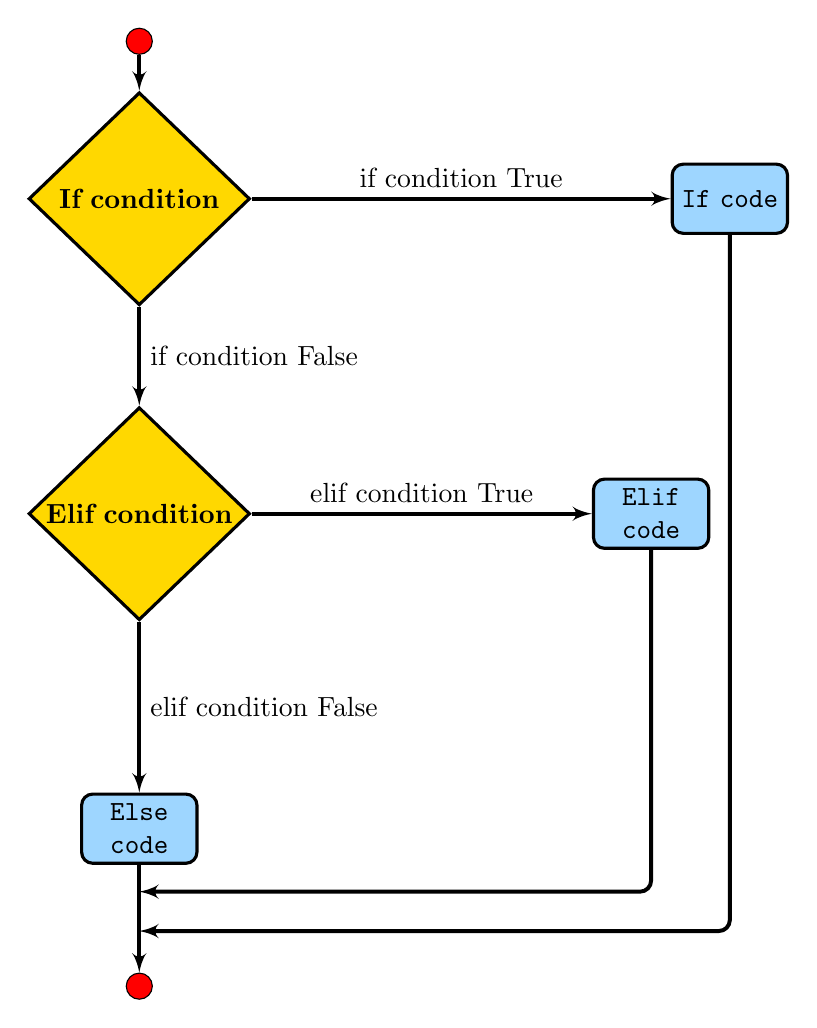
\begin{tikzpicture}[node distance = 1cm, auto]
    \node [startend] (start) {};
    \node [question, below of=start, node distance=2cm] (ifcond) {\textbf{If condition}};
    \node [question, below of=ifcond, node distance=4cm] (elifcond) {\textbf{Elif condition}};
    \node [operation, below of=elifcond, node distance=4cm] (else) {\texttt{Else code}};
    \node [startend, below of=else, node distance=2cm] (end) {};
    \node [operation, right of=ifcond, node distance=7.5cm] (ifcode){\texttt{If code}};
    \node [operation, right of=elifcond, node distance=6.5cm] (elifcode){\texttt{Elif code}};
	\node [coord, below of=else, node distance=0.8cm](c1){};
	\node [coord, below of=else, node distance=1.3cm](c2){};

    \path [line] (start) -- (ifcond);
    \path [line] (ifcond) -- node {if condition True} (ifcode);
    \path [line] (ifcond) -- node {if condition False}(elifcond);
    \path [line] (elifcond) -- node{elif condition True}(elifcode);
    \path [line] (elifcond) -- node{elif condition False}(else);
    \path [line] (ifcode)|-(c2);
    \path [line] (elifcode)|-(c1);
    \path [line] (else) -- (end);
\end{tikzpicture}
}
\end{center}

\vspace{-20pt}
\caption{A generic ``if'' statement flow chart}
%\vspace{-10pt}
\label{fig:iffc}
\end{figure}

\noindent Note: you can have as many `{\tt elif}' statements in an `{\tt if}' construct as you like, but only one `{\tt else}' (this should make sense if you think about it). Neither statement is required though and each use case will define how the conditions should be approached. \\

\noindent Also note: unlike in some programming languages, in \texttt{Python} you do not need to spell out where the {\tt if} condition stops, i.e. there is no {\tt endif} statement. This is because the condition only applies to the indented lines of code.

% \noindent Below is an example of the combination of `if', `elif' and 'else' conditions and how they can be used.
% \begin{lstlisting}[style=PY]
% In [1]: if condition:
% 	        # indented code block 1
%         elif condition:
% 	        # indented code block 2
%         else:
% 	        # indented code block 3
% \end{lstlisting}

\noindent Here is a simple example of how to use an if statement (notice the structure of colons and indentation above (see Section~\ref{indents})): 
\begin{lstlisting}[style=PY]
In [2]: # Define a list of integers
        list1 = [0, 1, 2, 4, 5]
    
        # Test if the list contains 1 
        if 1 in list1:
            print('There is a one in list1')
        else:
            print('There is not a one in list1')
	    
\end{lstlisting}

\noindent Now run the cell, and you should receive the following output. 
\begin{lstlisting}[style=PY_out]
        There is a one in list1
\end{lstlisting}  
\noindent Now edit the cell and change \texttt{list1} to the following.
\begin{lstlisting}[style=PY]
        list1 = [0, 10, 2, 4, 5]
\end{lstlisting}
Running the code again then gives.
\begin{lstlisting}[style=PY_out]
        There is not a one in list1
\end{lstlisting}  
As you will see if you have done the task correctly, the `{\tt if}' condition was satisfied in the first case. In the second case it was not, hence the `{\tt else}' block was executed.\\

\noindent Here is another example, this time using an `{\tt elif}' statement (at this point you might want to revise Boolean statements from session 1). Note that this example introduces a way to do nothing in a code block, \texttt{\color{mygreen}pass}.
\begin{lstlisting}[style=PY, escapechar=\%] 
In [3]: # Define a variable containing an integer 
        a = 50
        
        # Test the value of the variable a
        if a == 50:
            print( 'Variable a is 50' )
        elif a > 100:
            print( 'Variable a is more than 100' )
        # Note that the next two lines do nothing, and can be omitted
        else:
            pass  # do nothing

        print ('Finished')
\end{lstlisting}

\noindent Running the code should produce the following result.
\begin{lstlisting}[style=PY_out]
        Variable a is 50
        Finished
\end{lstlisting}  
Now change {\it a} in the code to the following.
\begin{lstlisting}[style=PY]
        a = 120
\end{lstlisting}
\noindent Running it a second time should produce the following result.
\begin{lstlisting}[style=PY_out]
        Variable a is more than 100
        Finished
\end{lstlisting}  
\noindent As you can see the `{\tt elif}' condition was met and block executed.\\
\noindent Now change variable {\tt a} to the following.
\begin{lstlisting}[style=PY]
        a = 100
\end{lstlisting}
\noindent Now when running the code the following should appear.
\begin{lstlisting}[style=PY_out]
        Finished
\end{lstlisting}  
\noindent Now that the variable \texttt{a} is neither 50 or greater than 100, the `{\tt else}' condition is executed. In this case the code is simply \texttt{\color{mygreen}pass} which does nothing and continues with the remaining code. Pass is rarely advised(!) but if you were to leave this blank then an indentation error would occur. Try the example below and see what happens when you run it.
\begin{lstlisting}[style=PY, escapechar=\%]
In [4]: # Define a variable containing an integer 
        a = 10
        
        # Test the value of the variable a
        if a %\textbf{==}% 50:
            print('Variable a is 50')
        elif a > 100:
            print('Variable a is more than 100')

        print('Finished')
\end{lstlisting}
\noindent The example above should show you that you don't \textbf{have} to include `{\tt else}' statements with an `{\tt if}' statement, often there is no need for one. \\
You don't just have to use singular conditions for `{\tt if}' and `{\tt elif}' statements, you can combine conditions together using \texttt{and} \texttt{or} or any other Boolean combination, as in the following:
\begin{lstlisting}[style=PY]
In [5]: # Define a tuple of names 
        b = ("Neil", "Edwin", "Michael")
        
        # Test if certain names are within the tuple
        if "Edwin" or "Buzz" in b:
            print("Edwin 'Buzz' Aldrin was the second man on the moon.")
        # Note that the next two lines do nothing, and can be omitted
        else:
            pass
\end{lstlisting}
\noindent If the code above was run, the text would be printed if tuple {\tt b} contained `Edwin' or `Buzz'. The Boolean \textbf{\color{orange}not} operator could be used to reverse the output i.e True becomes False and vice-verse. For example the above code could be changed to:
\begin{lstlisting}[style=PY]
In [6]: # Define a tuple of names
    # Test if certain names are within the tuple
    if "Edwin" or "Buzz" not in b:
        print("One of his names is missing from the list!")
    # Note that the next two lines do nothing, and can be omitted
    else:
        None
\end{lstlisting}

\newpage
\begin{lstlisting}[style=PY]
In [7]: # Define a tuple of names
    b = ('Neil', 'Edwin', 'Michael')
    # Test if certain names are within the tuple
    if 'Neil' and 'Edwin' in b:
        print('Neil Armstrong and Edwin \'Buzz\' Aldrin were the first 
               men to set foot on the moon.')
    # Note that the next two lines do nothing, and can be omitted
    else:
        None
\end{lstlisting}
This time, the use of \textbf{\color{orange}and} prints the text since both conditions have been met. 
Here, we have used {\color{mygreen}\textbackslash'} to allow a quotation mark inside a string. The backslash tells \texttt{Python} to ignore parts of its own syntax and just use it as text within the string. Alternatively, you can define the string with double quotation marks to use a single quotation mark in the string, and vice versa. \\
\noindent Additionally you can combine (or ``nest'') `if' statements for example below:
\begin{lstlisting}[style=PY]
In [8]: # Define a list of numbers
        q = [2, 4, 6, 8]
        
        # Test the contents of the list with nested if statements
        if 2 in q:
            if 4 in q:
                if 6 in q:
                    if 8 in q:
                        print ('2, 4, 6 and 8 are in q')
                    else:
                        print ('2, 4 and 6 are in q')
                else:
                    print ('2 and 4 are in q')
            else:
                print ('2 is in q')
        # Note that the next two lines do nothing, and can be omitted
        else:
            pass
\end{lstlisting}
\noindent The indentations also help you see what is happening when using multiple \texttt{`if'} statements, (i.e. they make the code more `readable'), since each corresponding pair of \texttt{'if'} and \texttt{'else'} statements line up.

\subsection{Exercises}
\subsubsection{Exercises (with worked answers)}
\label{ifexercises}
\noindent Try the following examples. (The solutions can be found in section~\ref{workedanswerslab3}).
\begin{enumerate}
\item Create a list of names called \texttt{nlist}, then create a string variable called \texttt{myname}. Use an \texttt{if} statement to check if \texttt{myname} is not in \texttt{nlist}. If \texttt{myname} is not in the list, add the name to the list and print the list. If it is within the list, print the list. (At this point, you might need to revise the {\tt append} command from session 2.
\item
\begin{enumerate}
\item Set a variable called {\tt myscore} and assign an integer of between 0 and 100 to it. Then using {\tt  if} statements print (`You have a first') if {\tt myscore} is 70 or above, `You have a 2:1' if {\tt myscore} is between 60 and 69, `You have a 2:2' if {\tt myscore} is between 50 and 59, `You have a third' if {\tt myscore} is between 40 and 49 and  `You have a not passed' if {\tt myscore} is below 40.
\item Adapt your code so that if {\tt myscore} is above 100 or below 0, it replies that `{\tt myscore} is not within the correct boundaries'.
\item Adapt the code so that it asks for, and accepts, a value from the user. This value can be an integer or float.
\end{enumerate}
\end{enumerate}

\subsubsection{Exercises (other)}
\begin{enumerate}
    \item W3Basic1 - A leap year is defined as a year which is:
    \begin{itemize}
        \item Divisible by 4. \textbf{and}
        \item \textbf{Not} divisible by 100. \textbf{Unless} 
        \item It is divisible 400.
    \end{itemize}
    Using a single Jupyter cell, write a section of code that allows the user to input a year, then outputs `True' if the year is a leap year or `False' if it is not. [Hint: Make use of the modulo operator \%, if you have not come across modulo arithmetic the Wikipedia page is pretty good!]
    \item W3Basic2 - Write some \texttt{Python} commands in a Jupyter cell to check if an input number is positive, negative or zero.
\end{enumerate}

\section{While Loops}
When we want to perform a repetitive task in computing we call upon loops. Using loops incorrectly in your code can lead to ``infinite loops'', so please have a look at section \ref{sec:infiniloop} to remind yourself what to do if that happens.

There are two basic types of loop: {\tt while} loops and a {\tt for} loops. A while loop executes a piece of code while a condition is considered true.

\begin{figure}[h]
\begin{center}
\resizebox{0.4\linewidth}{!}{
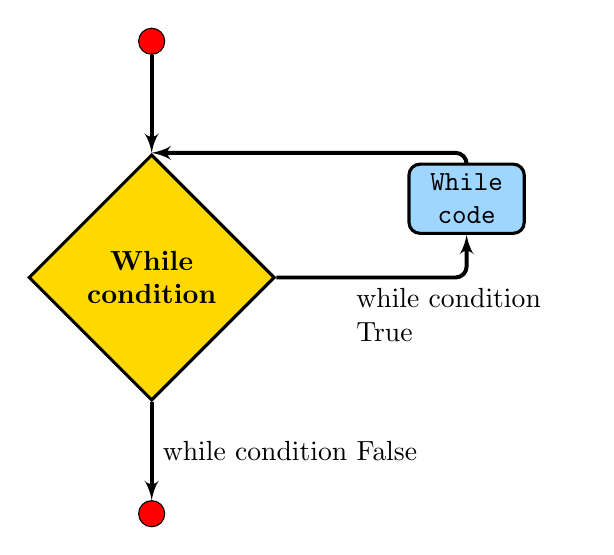
\begin{tikzpicture}[node distance = 3cm, auto]
    \node [startend] (start) {};
    \node [question, below of=start, node distance=3cm] (while) {\textbf{While condition}};
    \node [coord, right of=while, node distance=4cm] (c1){};
    \node [operation, above of=c1, node distance = 1cm] (wcode) {\texttt{While code}};
    \node [startend, below of=while] (end) {};

    
    \path [line] (start) -- (while);
    \path [line] (while) -| node [below,text width =2.8cm]{while condition True} (wcode);
    \path [line] (wcode.north) |- (while.north);
    \path [line] (while) -- node {while condition False}(end);
\end{tikzpicture}
}
\end{center}
\caption{While loop flow chart}
\label{fig:wlfc}
\end{figure}
\vspace{1cm}
\noindent Until the `{\tt while}' condition is declared false, the code continues to execute the code block inside the \texttt{while} loop. In some cases a counter is used to make sure the condition will be declared false at some point (if it is never declared false, the code enters an infinite loop).  \\
\noindent In some cases an `{\tt else}' statement is used to invoke another code block, i.e. when the opposite of the {\tt while} condition is true. A basic flow chart in figure \ref{fig:wlfc} shows a while loop. Note the need for colons after the condition, and indented executable code (as was the case with the {\tt if} statement). \\

\noindent An example of a while loop can be seen below:
\begin{lstlisting}[style=PY]
In [1]: while condition:
            # code block 1
        else:
            # code block 2
\end{lstlisting}
Notice that you can also follow a while loop with an if statement. This essentially says "while the condition is true: execute the while block, once it is not true: execute the else block". \\


\noindent Try to work out what these while loops do and add appropriate comments:
\begin{lstlisting}[style=PY]
In [2]: x = 0
        while x <= 12:
            print(x)
            x = x + 1

        print('Done')
\end{lstlisting}
\noindent The example below contains an `if' statement nested in a while loop.
\begin{lstlisting}[style=PY]
In [3]: i = 1
        while i < 10:
            if i%2 == 0:
                print (i, ' is an even number')
            else:
                print (i, 'is an odd number')
            i = i + 1
\end{lstlisting}

\noindent In the example above \texttt{i = i +1} is used, this takes the variable \texttt{i} and adds one to it, an alternative syntax is:

\begin{lstlisting}[style=PY]
In [4]: i = 1
        i += 1
        i
\end{lstlisting}
\begin{lstlisting}[style=PY_out]
Out[4]: 2
\end{lstlisting}

\noindent The use of \texttt{i += n}, takes variable \texttt{i} and adds \texttt{n} to it and reassigns it to variable \texttt{i}. The examples below show how to similarly take a variable, and add, subtract, multiply or divide, then reassign the new value to that variable. These commands can be useful for counters.

 
\begin{lstlisting}[style=PY]
In [5]: i -= 1
        i
\end{lstlisting}
\begin{lstlisting}[style=PY_out]
Out[5]: 1
\end{lstlisting}
\begin{lstlisting}[style=PY]
In [6]: i *= 5
        i
\end{lstlisting}
\begin{lstlisting}[style=PY_out]
Out[6]: 5
\end{lstlisting}
\begin{lstlisting}[style=PY]
In [7]: i /= 2.0
        i
\end{lstlisting}
\begin{lstlisting}[style=PY_out]
Out[7]: 2.5
\end{lstlisting}


\subsection{Exercises}

\begin{enumerate}
    \item W3Basic3 - Write some code to do the following:
        \begin{enumerate}
            \item Ask a user to enter a start number, end number, and interval (i.e. step size).
            \item Then print out a series starting and ending at the defined values in steps of the desired interval.
        \end{enumerate}
\end{enumerate}

\newpage

\section{For Loops}
For loops are similar to while loops but they work through items in a sequence, executing a block of code each time. You will be using them a lot in this module.

\noindent {\it If you have not read the while loop section yet, please do so, as this section won't make sense otherwise!}

\vspace{1cm}
\begin{figure}[H]
\begin{center}
\resizebox{0.5\linewidth}{!}{
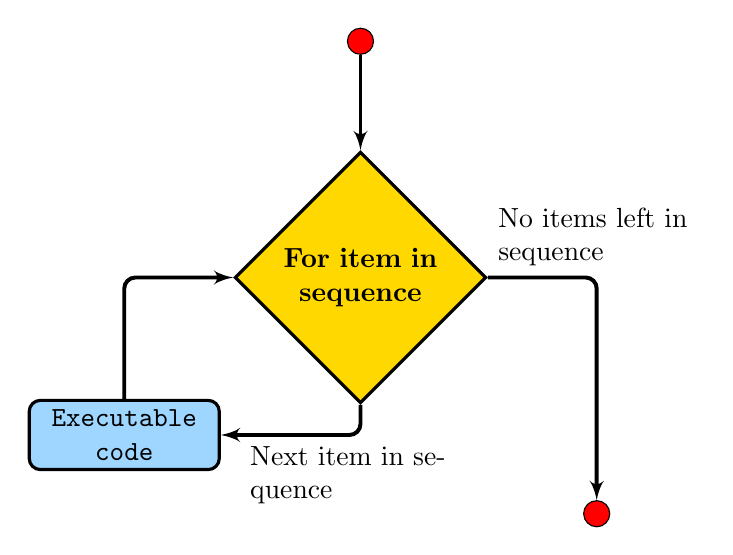
\begin{tikzpicture}[node distance = 3cm, auto]
    \node [startend] (start) {};
    \node [question, below of=start, node distance=3cm] (for) {\textbf{For item in sequence}};
    \node [coord, below of=for, node distance=2cm] (c1){};
    \node [operation,text width=6.2em, left of=c1, node distance = 3cm] (fcode) {\texttt{Executable code}};
    \node [startend, below of=for, right of=for] (end) {};

    
    \path [line] (start) -- (for);
    \path [line] (for) |- node [below,text width =2.8cm]{Next item in sequence} (fcode);
    \path [line] (fcode) |- (for);
    \path [line] (for) -| node [above,text width = 2.5cm]{No items left in sequence}(end);
\end{tikzpicture}
}
\end{center}
\caption{For loop flow chart}
\label{fig:flfc}
\end{figure}

\noindent One way to think of a for loop is that in the background a counter is active, performing a task until the counter reaches a certain number that is equal to the total items in a sequence. Just like \texttt{if} statements and while loops, for loops are written in the same way with a block, indented in to tell \texttt{Python} what to do.\\

\noindent Similar to \texttt{'while'} loops `else' statements can be used to perform an operation after the loop is complete. \texttt{'for'} loops can also be nested within each other to perform operations. An example layout of a for loop can be found below.

\begin{lstlisting}[style=PY]
In [1]: for item in sequence:
	        # code block 1
        else:
	        # code block 2
\end{lstlisting}
The sequence can be a range of numbers, a list, tuple, or even a string. The item is commonly referred to as `\texttt{i}' as it is a counter starting at the beginning of the sequence and stopping at the end, however we can name this counter variable anything within reason. (Because {\tt i} is so commonly used as a counter, \texttt{Python} uses {\tt j} to denote complex numbers, see session 1). \\

\newpage

\noindent This example prints out the result of a simple maths operation on a list of numbers.
\begin{lstlisting}[style=PY]
In [2]: # Define a list of numbers
        numberlist = [1, 2, 3, 4, 5, 6]
        
        # Loop over the elements in the list squaring them
        for i in numberlist:
            print (i*i)
\end{lstlisting}
This example prints each letter of a word on a new line. Here the sequence is a string, i.e. `{\tt word}'.

\begin{lstlisting}[style=PY]
In [3]: # Loop over the characters in a string printing each
        for letter in 'word':
            print (letter)
\end{lstlisting}
This example loops through a list of strings, printing the string and then it's length. Here the sequence is a list, i.e. `{\tt list1}'.
\begin{lstlisting}[style=PY]
In [4]: # Define a list of strings
        list1 = ['Monty', 'Python', 'Spam', 'Eggs']
        
        # Loop over the list printing the word and it's length
        for word in list1:
            print (word, 'has', len(word), 'letters')
\end{lstlisting}

\section{Format strings}
In the above example you will notice that when printing out the strings and integers or floats etc., parentheses and quotation marks are also printed. This is due to the fact we are mixing data types when printing, a way around this is to assign non-string types to variables and then use \emph{format strings} to print them.

A \emph{format string} is preceded by the letter f, and the variables to be
printed are enclosed in curly braces \{\}, e.g.
\begin{lstlisting}[style=PY]
  In [1]: # Example of format strings
  # Define a list of strings
        list1 = ['Monty', 'Python', 'Spam', 'Eggs']
        
        # Loop over the elements in the list 
        for word in list1:
        
            # Get word length
            wl = len(word)
            print(f'{word} has {wl} letters')
\end{lstlisting}

You can optionally specfify the format of the string conversion by following the variable name with a format qualifier, such as `:3d' to print a 3-digit integer, or `:5.4f' for a float with format x.xxxx.
\begin{lstlisting}[style=PY]
  In [1]: # Example of format strings with optional format specifier
  print(f'root 2 to 6 sig figs = {2**0.5:6.5f}')
\end{lstlisting}

%% The percentage symbol known as the {\bf modulo operator} in \texttt{Python}, allows for these data types to be inserted into a string, think of them as place holders. After the initial string there is a percentage symbol and a tuple or list containing the variables needed. Within the string itself you will see \texttt{\%s} the s converts the item in the tuple or list to a string for the print command, the order of the percentages in the string match the variables entered in the tuple or list, see example below. Some of the other commands are displayed in Table~\ref{tab:ms} they all allow variable values to be displayed in strings with different formatting.

%% \begin{lstlisting}[style=PY]
%% In [1]: # Define a list of strings
%%         list1 = ['Monty', 'Python', 'Spam', 'Eggs']
        
%%         # Loop over the elements in the list 
%%         for word in list1:
        
%%             # Get word length
%%             wl = len(word)
%%             print('%s has %s letters'%(word, wl))
%% \end{lstlisting}
%% %\begin{tcolorbox}[colback=red!5!white,colframe=red!75!black]
%% %\end{tcolorbox}
%% \begin{table}[H]
%% \begin{center}
%% \begin{tabular}{|l | p{12cm}|}
%% \hline
%% \texttt{\%s} & Converts variable to string.\\\hline
%% \texttt{\%i} & Converts variable to an integer in the string. To specifiy values use \texttt{\%ni} the n specifies how many characters are taken up for example if n was 5 and the variable was a 3 digit number two spaces would be in front of the variable or if n was 05 two zeros would be in front of the variable. If \texttt{\%i} is used the integer is just displayed.\\\hline
%% \texttt{\%d} & Converts variable to a decimal integer in the string. Similar to \texttt{\%i}\\\hline
%% \texttt{\%e} & Converts variable to an exponent in the form \texttt{w.nn e+xx} for use in string. If you wish to specify decimal places use the following \texttt{\%n.de}, the number would have d decimal places and the exponent n digits. E.g. \texttt{`\%2.3e'\% (45673)} would output \texttt{4.567e+04}.\\\hline
%% \texttt{\%f} & Converts variable to a float for use in string. To specify number of decimal places use \texttt{\%1.nf}, with n being number of decimal places e.g. \texttt{`\%1.2f'\% (25)} with output of \texttt{25.00}.\\\hline
%% \end{tabular}
%% \caption {String variable operators}
%% \label{tab:ms}
%% \end{center}
%% \end{table}

%% \begin{tcolorbox}[colback=red!5!white,colframe=red!75!black]
%% Although not needed for this sub-module, for completeness we note here that there is an alternative approach to the modulo command, the \texttt{.format} string function. It is much more powerful in usability, can have syntax uses and repetition of the same variable. and can inherently understand tuples. Additionally, as it is a function (Section~\ref{sec:function}), it can be used with map and other functions for more advanced \texttt{Python}. 

%% Again for completeness: if you're using \texttt{Python} $\geq$3.7 (the University isn't!) format strings have been introduced. These behave similarly to \texttt{.format} but are much more readable. To use a format string proceed your string by an f, i.e. \texttt{f''}.

%% \begin{lstlisting}[style=PY]
%% In [2]: # Define a list of numbers
%%         lst = [1.0, 9.9, 3.14159]
%%         approx_pi = lst[-1]
        
%%         # Using format
%%         print('The first element is {x}'.format(x=lst[0]))
%%         print('The last element is {x}'.format(x=approx_pi))
        
%%         # Using format strings (Python 3.7 or greater exclusive!)
%%         print(f'The first element is {lst[0]}')
%%         print(f'The last element is {approx_pi}')
%% \end{lstlisting}

%% \end{tcolorbox}

\newpage

\section{Range command}
\label{sec:range}
The \texttt{range} command allows you to create a list of numbers. You will be using it a lot in this module. Below are a few examples of the range command in action:
\begin{lstlisting}[style=PY]
In [1]: # Define a list using the range command containing 
        # integers from 0 to 9 (inclusive)
        list1 = range(10)
        print(*list1)
\end{lstlisting}
\begin{lstlisting}[style=PY_out]
        0 1 2 3 4 5 6 7 8 9
\end{lstlisting}

\noindent This is the range command in its simplest form, \texttt{range(j)}, it creates a list starting at zero with increments of 1 going all the way up to \texttt{j-1}. Note the \texttt{*}, this expands all the elements of a list (or tuple) rather than printing the list itself.

\begin{lstlisting}[style=PY]
In [2]: # Define a new list using range with a start and end point
        list2 = range(1, 11)
        print(*list2)
\end{lstlisting}
\begin{lstlisting}[style=PY_out]
        1 2 3 4 5 6 7 8 9 10
\end{lstlisting}
The above example shows the {\tt range} command with start and end declarations, i.e. the command \texttt{range(i,j)} creates a list starting at \texttt{i} and ending at \texttt{j-1} with increments of 1.
\begin{lstlisting}[style=PY]
In [3]: # Define a list using range with a start, end and step size
        list3 = range(0, 10, 2)
        print(*list3)
\end{lstlisting}
\begin{lstlisting}[style=PY_out]
        0 2 4 6 8
\end{lstlisting}
This final example shows the {\tt range} command with all of its inputs. \texttt{range(i,j,k)} where \texttt{i} is the start number, \texttt{j} declares the end (\texttt{j-1}) and \texttt{k} shows the step size. All of the inputs need to be integers as the range command only works with integers and not floats.\\
Table \ref{tab:rc} shows all the variants for the range command.
\begin{table}[H]
\begin{center}
\begin{tabular}{|l | p{7cm}|}
\hline
\multicolumn{2}{|c|}{\color{blue}Note: range command only works with integers}\\\hline
\texttt{range(j)} & Creates a list starting at 0 and ending at \texttt{j-1} with increments of 1\\\hline
\texttt{range(i,j)} & Creates a list starting at \texttt{i} and ending at \texttt{j-1} with increments of 1\\\hline
\texttt{range(i,j,k)} & Creates a list starting at \texttt{i} and ending at \texttt{j-1} with increments of \texttt{k}\\\hline
\end{tabular}
\end{center}
\caption {Range command}
\label{tab:rc}
\end{table}
\noindent Below is an example using the {\tt range} command and nested {\tt for} loops.
\begin{lstlisting}[style=PY]
In [4]: # Loop through a range 
        for i in range(2,6):
        
            print (f'{i} times table')
	        
            # Within the outer loop, loop over numbers between 1-10 
            for j in range(1,11):
	        
	        # Compute product of outer loop and inner loop integers
                num = i*j
		print (f'{i} x {j} = {num}')
\end{lstlisting}

\subsection{Using the separator command}

The separator command in {\tt print} is a nice feature.

\begin{lstlisting}[style=PY]
In [5]: # Define a list from a range 
        list4 = range(1, 11)
        
        # Print the list separated by whitespaces and commas
        print(*list4, sep=' , ')
\end{lstlisting}
\begin{lstlisting}[style=PY_out]
        1 , 2 , 3 , 4 , 5 , 6 , 7 , 8 , 9 , 10
\end{lstlisting}
The separator can indeed be anything, including ridiculous things.
\begin{lstlisting}[style=PY]
In [6]: print(*list4, sep='  [banana] ')
\end{lstlisting}
\begin{lstlisting}[style=PY_out]
        1 [banana] 2 [banana] 3 [banana] 4 [banana] 5 [banana] 6 [banana] 7 [banana] 8 [banana] 9 [banana] 10
\end{lstlisting}

\subsection{Exercises}
\subsubsection{Exercises (with worked answers)}
\label{rangeexercises}
\noindent Try the following examples. (The solutions can be found in section \ref{workedanswerslab3}).
\begin{enumerate}
\item Use a {\tt for} loop and the {\tt range} command to find the first 10 terms of the following series: $$\frac{1}{2}+\frac{1}{4}+\frac{1}{8}+\frac{1}{16}+\ldots$$
\item Using range, a for loop and if, elif and else conditions, print: \texttt{`1 potato 2 potato 3 potato 4, 5 potato 6 potato 7 potato more.'}.
\item Write an program that asks for and inputs the user's name. It then checks if the users name is within a list of names. If the name is in the list, it should then print a message telling the user that their name is on the list. If not, add the users name to the list and inform them their name has been added to the list.
\end{enumerate}

\subsubsection{Exercises (other)}

W3Basic4 - Write a program using a for loop that allows the user to input a word then print out the word backwards.
 
\section{Functions}
\label{sec:function}
There are already functions built into \texttt{Python}, {\tt print} for instance. However, you can also define your own functions. Functions are repeatable blocks of code that can be used over and over again. \\

\noindent Functions are defined using colons and indentation, similar to \texttt{if} statements and for/while loops. You can define parameters (arguments) to be used within the function, a general example is below:
\begin{lstlisting}[style=PY]
In [1]: def function_name( parameter1, parameter2,....):
            # block of code
            return statement(s)
\end{lstlisting}
Then to call upon them in the script use the following command.
\begin{lstlisting}[style=PY]
In [2]: function_name(x_parameter1, x_parameter2, ...)
\end{lstlisting}
Arguments don't have to be used, however they are used when performing tasks on different data points etc. An example not containing arguments is below:
\begin{lstlisting}[style=PY]
In [3]: def GameOver():
            print ('Game Over!')
            return

        GameOver()
\end{lstlisting}
Running the above code, will simply print out \texttt{Game Over!} when called upon, this simple example shows how repeatable code can save time as you don't have to write out the print command over and over again.

{\bf Be careful not to call your new function something that is already built in to \texttt{Python}!} You can check whether a function name is already in use by typing {\tt help(NameToCheck)}. As your coding gets more advanced, you will feel the benefits of using functions more and more. \\

\noindent The following example uses arguments:
\begin{lstlisting}[style=PY]
In [4]: def cubed(alist):

            # Loop over elements of the argument
            for i in range(len(alist)):
            
                # Cube the element and reassign it to the list
                alist[i] = alist[i]**3
                
        # Define a list of numbers to be used in the function
        numbers = list(range(5))
        
        # Cube the numbers using the user defined function
        cubed(numbers)
        print(numbers)
\end{lstlisting}

\noindent Running the code would output, \texttt{[0, 1, 8, 27, 64]}. Here, we have passed in the \texttt{numbers} variable, which was then assigned to a variable called \texttt{alist} in the function which is entirely internal to the function. 

\begin{lstlisting}[style=PY]
In [5]: def series(para):

            # Define a variable to hold the sum
            asum = 0
            
            # Loop over elements of the argument
            for i in para:
            
                # Sum the squares of the argument
                asum += para[i]**2
                
        # Define a list of numbers to be used in the function
        numbers = list(range(5))
        # Find the sum of the series defined by the function
        series(numbers)
        print(asum)
        
\end{lstlisting}
This code finds the sum of the series $x^{2}$, however if you have copied the code and run it yourself, you will find a NameError has occurred. This is due to \texttt{asum} not being a global variable i.e. it is only a variable within the function. To use this variable in different parts of the code we will need to return it, which will pass it back out of the function and assign it to another variable (this is part of a greater concept in coding called `Namespaces' [scopes in other languages] which will be covered later if people are interested).

\newpage

\begin{lstlisting}[style=PY]
In [6]: def series(para):

            # Define a variable to hold the sum
            asum = 0
            
            # Loop over elements of the argument
            for i in para:
            
                # Sum the squares of the argument
                asum += para[i]**2
                
            return asum
	    
        # Define a list of numbers to be used in the function
        numbers = list(range(5))
        
        # Find the sum of the series defined by the function
        series_sum = series(numbers)
        print (series_sum)
\end{lstlisting}

The return statement outputs the value, then we need to assign it to a variable, in this case \texttt{series\_sum}, to then read from it. If we wanted to return multiple values we can do the following:
\begin{lstlisting}[style=PY]
In [7]: def timestable(number):

            # Compute the products of the number in the argument
            a = number * 2
            b = number * 3
            c = number * 4
            d = number * 5
            
            return a, b, c, d
	        
        # Compute 5 multiplied by 2-5 (inclusive) using the function
        q, w, e, r = timestable(5) 
\end{lstlisting}
Using commas we can assign multiple variables with multiple returns. Side note here, a function returning multiple variables actually returns a tuple containing the returns.

\subsection{Exercises}
\begin{enumerate}
    \item W3Basic5 - Repeat W3Basic1 using a function.
    \item W3Basic6 - Repeat W3Basic2 using a function.
    \item W3Basic7 - Write a new function.
    \begin{enumerate} 
        \item It must take two parameters, a pay rate, and number of hours worked.
        \item Make it return the total pay.
        \item Alter the function so that any hours over 40 is paid at 1.5 times the normal rate.
    \end{enumerate}
\end{enumerate}

\section{Signpost} 

You need to have at least got to this point by the end of the lab session in week 3. You now have all the tools needed to finish the first assessment.

\begin{tcolorbox}[colback=red!5!white,colframe=red!75!black]
\section{Lambda statement}
The lambda statement is basically a single line function for use with expressions. The function can be expressed in the following way, with an arbitrary number of arguments:
\begin{lstlisting}[style=PY]
In [1]: function_name = lambda argument1, argument2, ...: expression
\end{lstlisting}
An example of a lambda statement:
\begin{lstlisting}[style=PY]
In [2]: root = lambda x, n: x**(1 / n)

        print (root(2,2))
        print (root(2,3))
        print (root(2,4))
\end{lstlisting}
Evidently, they are very similar to the function command but can be more succinct for simple repeatable calculations.
\end{tcolorbox}

\section{Dictionaries}
Although not used heavily in this course, dictionaries are one of the most powerful data structures in \texttt{Python}.

\noindent The dictionary data type holds pairs of {\bf keys} and {\bf values}, and are defined using curly braces `\{ \}'. The key, value pairs are defined as items with commas and a key separated by a `:'.\\

\noindent A dictionary cannot have any repeating keys, however it can have repeating values i.e. different keys can have the same value. An example of how to create a dictionary can be seen below, it also shows how to retrieve information from a particular key. Note that the values do not need to be strings, they can be numbers (e.g. phone numbers), or even \texttt{Python} objects.  
\begin{lstlisting}[style=PY]
In [1]: # Define a dictionary
        dictionary = {'key':'value', 'another key':'another value'}
        
        # Extract a value
        dictionary['key']
\end{lstlisting}
\begin{lstlisting}[style=PY_out]
Out[1]: 'value'
\end{lstlisting}
\begin{lstlisting}[style=PY]
In [2]: # Extract another value
        dictionary['another key']
\end{lstlisting}
\begin{lstlisting}[style=PY_out]
Out[2]: 'another value'
\end{lstlisting}

\newpage

\begin{lstlisting}[style=PY]
In [3]: # Define a dictionary with 2 of the same key
        double = {'key':1, 'key':2}
        double
\end{lstlisting}
\begin{lstlisting}[style=PY_out]
Out[3]: {'key': 2}
\end{lstlisting}
From the example above, you can see that if there is a repeating key the last value will be taken. Below are some more examples of manipulating dictionaries.
Here we reassign a string to an existing key overwriting the old value.
\begin{lstlisting}[style=PY]
In [1]: # Define a new dictionary
        dictionary = {'key':'old','Hello':'World'}
        
        # Overwrite the value of 'key'
        dictionary['key'] = 'new'
        dictionary['key']
\end{lstlisting}
\begin{lstlisting}[style=PY_out]
Out[1]: 'new'
\end{lstlisting}
We can delete a key using \texttt{Python}'s \texttt{del} function. This function deletes what follows it from memory (technically only removes the label/memory address) and is not specific to dictionaries. If you have a list that is hogging memory, but you no longer need it you can free up that memory using the \texttt{del} function (sort of: memory management is a somewhat mystic art in \texttt{Python}, ask if you are interested).
\begin{lstlisting}[style=PY]
In [2]: # Delete the entry under the key 'Hello'
        del dictionary['Hello']
        dictionary
\end{lstlisting}
\begin{lstlisting}[style=PY_out]
Out[5]: {'key':'new'}
\end{lstlisting}
You can add new keys:
\begin{lstlisting}[style=PY]
In [6]: # Assign a new entry to the dictionary
        dictionary['Good'] = 'bye'
        dictionary
\end{lstlisting}
\begin{lstlisting}[style=PY_out]
Out[6]: {'Good':'bye','key':'new'}
\end{lstlisting}
You can get the length of the dictionary which corresponds to the number of key, value pairs.
\begin{lstlisting}[style=PY]
In [7]: # Get the length of the dictionary
        len(dictionary)
\end{lstlisting}
\begin{lstlisting}[style=PY_out]
Out[7]: 2
\end{lstlisting}
You can also wipe a dictionary completely without deleting the data structure itself thusly:
\begin{lstlisting}[style=PY]
In [8]: # Wipe the contents of the dictionary
        dictionary.clear()
\end{lstlisting}
\begin{lstlisting}[style=PY_out]
Out[8]: {}
\end{lstlisting}

Below is a set of examples showing how you can access specific parts of a dictionary and interact with them.
We can get a list containing the items.
\begin{lstlisting}[style=PY]
In [9]: # Define 2 dictionaries for manipulation
        dict1 = {'Hello':'World','Good':'Bye'}
        dict2 = {'Game':'Over','You':'Lose'}
        
        # Get the items in a dictionary
        list(dict1.items())
\end{lstlisting}
\begin{lstlisting}[style=PY_out]
Out[9]: [('Hello','World'),('Good','Bye')]
\end{lstlisting}
We can get a list containing the keys.
\begin{lstlisting}[style=PY]
In [10]: # Get a list of the keys of a dictionary
         list(dict2.keys())
\end{lstlisting}
\begin{lstlisting}[style=PY_out]
Out[10]: ['Game','You']
\end{lstlisting}
We can get a list containing the values.
\begin{lstlisting}[style=PY]
In [11]: # Get a list of the values of a dictionary
         list(dict1.values())
\end{lstlisting}
\begin{lstlisting}[style=PY_out]
Out[11]]: ['World','Bye']
\end{lstlisting}
We can test if a key is within a dictionary.
\begin{lstlisting}[style=PY]
In [12]: # Test if 'Hello' is in the first dictionary
         if 'Hello' in dict1
\end{lstlisting}
\begin{lstlisting}[style=PY_out]
Out[12]: True
\end{lstlisting}
\begin{lstlisting}[style=PY]
In [13]: # Test if 'Hello' is in the second dictionary
         if 'Hello' in dict2
\end{lstlisting}
\begin{lstlisting}[style=PY_out]
Out[13]: False
\end{lstlisting}
We can combine dictionaries with the update method.
\begin{lstlisting}[style=PY]
In [14]: # Combine the 2 dictionaries
         dict1.update(dict2)
         dict1
\end{lstlisting}
\begin{lstlisting}[style=PY_out]
Out[14]: {'Hello':'World','Good':'Bye','Game':'Over','You':'Lose'}
\end{lstlisting}
The \texttt{dict.items()} function lists all the keys and values as tuples. The \texttt{dict.keys()} and \texttt{dict.values()} functions give the keys and values of the dictionary respectively. Finally the \texttt{dict.update()} adds the keys and values from one dictionary to another. - note that the ''()'' is important - the {\tt .key} etc. operations will not do anything without them. Think back to the function we defined with no arguments, the same would be true there. \\

\begin{tcolorbox}[colback=red!5!white,colframe=red!75!black]
\subsection{A Note On Iterators}
Here we have taken a small amount of poetic license. As of \texttt{Python} 3 a number of \texttt{Python}'s inbuilt functions were changed to return an object called an iterator rather than lists or tuples. This can greatly increase performance when simply looping through a set of keys, values or items in a dictionary but can also lead to some confusion when working with these. This is why all calls to \texttt{.items}, \texttt{.values} and \texttt{.keys} above are wrapped with \texttt{list()}.

You can work with the elements inside an iterator without issue when looping through them but should you find yourself needing to extract all values into a list and print them you would find that a \texttt{Python} object were printed instead. This is shown below

\begin{lstlisting}[style=PY]
In [1]: # Define a dictionary containing arbitrary keys and values
        dict1 = {'a': 1, 'b': 2, 'c': 3}
        print(dict1.keys())
        print(dict1.values())
        print(dict1.items())
\end{lstlisting}
\begin{lstlisting}[style=PY_out]
        dict_keys(['a', 'b', 'c'])
        dict_values([1, 2, 3])
        dict_items([('a', 1), ('b', 2), ('c', 3)])
\end{lstlisting}

To avoid this you can simply convert to a list or indeed a tuple as shown above depending on whether they need to be mutable or not.

\end{tcolorbox}

\section{Advanced Exercises}

Helpful hint: checking the glossary and the world wide web, may help with these exercises.

\begin{enumerate}

\item Write a program where a user gets 3 chances to guess a password. If the password is correct print `Access Granted' and exit the loop, if incorrect print `Access Denied'. Modify the code so that after the third guess a message is displayed telling the user they have run out of guesses.
\item DNA sequence strings are made up of the letters A, T, G, and C. The DNA sequence strings have a complement string where the the letters are switched. A's become T's,
T's become A's, G's become C's, and C's become G's. For example, the complement
of TTATGGCGTA is AATACCGCAT. Write a function that produces a complement of a DNA string.
\item Using a dictionary create a phone book, with a key of names and numbers as values. Then write a function that searches the dictionary for a name, if the name exists, give options to call, edit or remove the contact. If call is selected, print \texttt{Calling}, and the name, to the screen. Whereas, if edit of remove are selected, edit the number or remove the contact respectively. If the name does not appear give the option to add the name to the dictionary. 

\end{enumerate}

\newpage
\section{Worked Examples}
\label{workedanswerslab3}
\begin{lstlisting}[style=PY]
# 3.3.1
# Question 1.
myname = 'Nick' # Your name goes here  
nlist = ['Amy', 'Tom', 'Nina', 'James']
if myname not in nlist:
	nlist.append(myname)
	print (nlist)
else:
	print (nlist)
	
# Question 2a.
myscore = 65 # Your score would go here
if myscore > 70:
	print ('You have a first')
elif 60 <= myscore <= 69:
	print ('You have a two:one')
elif 50 <= myscore <= 59:
	print ('You have a two:two')
elif 40 <= myscore <= 45:
	print ('You have a third')
elif myscore < 40:
	print ('You have not passed')
	
# Question 2b.
myscore = 65 # Your score would go here
if 70 <= myscore <= 100:
	print ('You have a first')
elif 60 <= myscore <= 69:
	print ('You have a two:one')
elif 50 <= myscore <= 59:
	print ('You have a two:two')
elif 40 <= myscore <= 45:
	print ('You have a third')
elif 0 <= myscore <=40:
	print ('You have not passed')
else:
	print ('myscore is not within the boundary of 0 and 100')
\end{lstlisting}	
\newpage
\begin{lstlisting}[style=PY]
# Question 2c.
myscore = float(input('What is your score? '))
if 70 <= myscore <= 100:
	print ('You have a first')
elif 60 <= myscore <= 69:
	print ('You have a two:one')
elif 50 <= myscore <= 59:
	print ('You have a two:two')
elif 40 <= myscore <= 45:
	print ('You have a third')
elif 0 <= myscore <=40:
	print ('You have not passed')
else:
	print ('myscore is not within the boundary of 0 and 100')

3.6.2 
# Question 1
series = 0
for i in range (1,11):
	series += ( 1/(2.0**i) )
	print (series) 

# Question 2
string = ''
for num in range(1, 8):
    
    if num in [1, 2, 3, 5, 6]:
        string += str(num) + ' potato '
    elif num == 4:
        string += '4, '
    else:
        string += '7 potato more.'
        
print(string)

# Question 3.
names = ['Tom', 'Jerry', 'Sarah', 'Julian']
uname = input('Name? :')
if uname in names:
	print ('Your name is on the list')
else:
	name.append(uname)
	print ('Your name has been added to the list')
\end{lstlisting}


\chapter{Python Modules and an Introduction to Plotting}
%\chapterauthor{PRATS}
\label{chap:modules}
\section{Learning Outcomes}

By the end of week 5, you should be able to:
%CHANGE - need to reword to be correct!

\begin{enumerate}
\item Know what Python modules are and what they are for. 
\item Know how to load Python modules.
\item Know how to find out what functions are inside a given module and how to get help with those functions.
\item Be familiar with \texttt{numpy}, \texttt{scipy} and \texttt{matplotlib} modules (especially \texttt{arange} from the \texttt{numpy} module).
\item Be familiar with the the {\tt random} module.
\item Be able to make basic plots.
\end{enumerate}

\section{What are modules?}

Modules are pieces of code that have been created by other developers that give Python more functions and abilities. They are generally open source, actively developed, and available for free. In serious programs they are indispensable! Replicating code that other people have already written is a pointless waste of time and money (if you're being employed). Often they will have been implemented in a far more memory and time efficient time way than would be possible without years of experience, possibly even interfacing with much faster C or C++ (numpy for instance) code under the hood.


% \noindent Longer answer...\\

% \noindent Think of Python like the main part of the Bridge Cafe (i.e. the bit behind the counter). There is lots of good stuff to buy from behind the counter, but sometimes you fancy a sandwich, and you'd pick that up from chilled cabinet to the right of the till.\\

% \noindent The cabinet can't exist without the Cafe, but the reverse is not true. In this analogy, the Cafe is the bare bones of Python (one where you can add two numbers, but you can't evaluate the cosine of an angle).\\

% %add section from Labsession2n3
% \noindent You can think of the sandwiches as functions within the {\tt cabinet} module. Functions inside modules save you from doing menial coding tasks. For example, you are fully capable of going to the co-op to buy bread, butter, salad, cheese, etc. and then making a cheese sandwich; but why would you bother to do that when someone has already solved the problem for you (assuming the financial outlay is the same)? In Python speak, we are talking about the {\tt cabinet.cheesesandwich} function. Although if the bridge cafe was like the world of open source programming, the sandwich would be free!\\

% \noindent You can also think of modules being menus that suggest things to eat (or code with) that hadn't occurred to you before. For example, might have thought you wanted {\tt cheesesandwich} when you walked up to {\tt cabinet}, but when you looked inside your eyes (and belly) were drawn to a falafal wrap. In Python speak, you have just run {\tt dir(cabinet)} and been given a list of all the other food items (or ``functions'') available. Tip: always keep an open mind when coding, there might well be other ways to get the job done better or faster (or both).\\

% \noindent Maybe a week later as you are reaching for {\tt falafalwrap} a friend asks you why you aren't going for {\tt brieandgrapebaguette}. You've never heard of mixing fruit with cheese before, but you decide to give it a try anyway. You are blown away by the taste sensation you've been missing. This experience is equivalent to using Google, or talking to your ATs/tutor/classmates, to discover new ways to code. Very soon, you'll be sharing your ideas with other people too. Sharing ideas is essential to the ``Open Source'' community. If kind people didn't make their codes available, there would be no Python.\\

% \noindent  Back to the Bridge... On another day, you feel like adding a packet of crisps to your lunch. You look in {\tt cabinet} and feel sad that there is no function there that can help. Fortunately, there is another module to hand: {\tt woodenstand}! Here is the function you are looking for: {\tt woodenstand.lightlysaltedkettlechips}. This example shows that there are several different modules and each are useful for different things. After all, there is no point taking up space in {\tt cabinet} with {\tt lightlysaltedkettlechips} because they don't need to be kept cold.\\

% \noindent  On another day, you feel like turning your back on crisps and sandwiches and wraps, you are craving chips. You look around for another module, predicting that it would be called {\tt fryup}. But it isn't there! Why not? Because we have run out of room on the Bridge. If they put in a frying station, there would be no room for chairs and tables and the {\tt selectionofcakes} function. This is equivalent of realising that if you try to load every possible module into Python then you'll have the maximum choice of goodies, but you'll have used up all the RAM (memory) and won't have any where to ``sit and eat'' (i.e. run your program). So you need to be selective (or get a better computer).\\

% \noindent  You might have noticed that on the counter they sell commercial flapjack  to the left of the till and homemade flapjack in the covered area next to the cold cabinet. (it is not clear why this duplication exists, but it does, and as customers, we've learned to accept it.) The homemade flapjack might well taste better (or be cheaper) than the one on the counter, so we need to tell Python (i.e. one of the lovely staff behind the bar) which one we want: to do this, we'd ask for  {\tt coveredarea.flapjack} rather than just {\tt flapjack}. The fact that there are many cases of functions in different modules that have the same name is one of the downsides to Python. \\

% \begin{figure}
% 	\centering
% 	\includegraphics[width=14cm]{Figures/bridgePython.png}
% 	\caption{The various ``modules'' in the Bridge Cafe}
% \label{fig:be3}
% \end{figure}

\noindent A quick overview of modules: 
\begin{itemize}
\item Standard Python contains many built in functions, but does not contain everything you will need in your coding future.
\item Modules can be added to Python and contain dozens of functions.
\item Occasionally (but rarely, this is mostly avoided) function names are duplicated in different modules or between standard Python and a module. Even though they share a name the operation of these functions could be very different. Therefore, you have to be careful to use the correct version (by specifying the module name explicitly in the function call).
\item You should only import the modules that you need, and only import them once (loading modules multiple times and/or loading modules you don't need leads to wasted RAM).
\end{itemize}

\begin{tcolorbox}[colback=red!5!white,colframe=red!75!black]
Terminology gets a bit muddy from here on out... strictly a function is a self defined chunk of reusable code, as you have seen in the previous chapter. These modules in fact contain "methods", a term which will make far more sense if you progress to object-orientated \texttt{Python}. For simplicity we will use the two interchangeably, mostly focusing on mis-using "function" but don't be confused if you come across "method" in the future or online.
\end{tcolorbox}

\section{Common Python modules}

Modules we will cover in this course\footnote{We are using ``course'' rather than ``sub-module'' to avoid confusion with the topic of this lab session.} include: 
\begin{itemize}
\item {\tt matplotlib}: graphics tools to create and display plots. In Physics and Astrophysics it is frequently used to make plots for publications.
\item {\tt numpy}: data structures and mathematical resources not included in basic Python, for example cosine, exponentials etc. Some basics of {\tt numpy} will be discussed in this section but chapter \ref{chap:numpy} will provide a more comprehensive overview. 
\item  {\tt scipy}: scientific resources such as those needed in mathematical physics, e.g. bessel, gamma, beta functions, signal processing, integration, differential equation solving and statistics... (you will use {\tt scipy} a {\bf lot} in Scientific Computing in Y2).
\item  {\tt random} (Section~\ref{randommodule}): used to generate pseudo-random numbers within the Python environment. The module is very useful for generating random numbers quickly in a range of circumstances.
\item  {\tt pandas} (see Chapter~\ref{Chapter6}): allows you to work with data in something analogous to spreadsheets.
\item  {\tt os}: allows you to interface Python with Unix, for example if you want to load up certain types of file into your Python code.
\end{itemize}

%\item{\tt math} (Section~\ref{mathmodule}) does much the same as {\tt numpy} (and hence to the maths functions inside {\tt pylab}) so you probably won't need it. But occasionally {\tt numpy} will not have (or seem not to have) what you need, see example 3 in Section~\ref{INeedMaths}.
\newpage
\noindent Here are some additional modules that you may come across, especially if you are working on the optional challenges or an independent project. Although it is absolutely fine to use these, or other, non-standard modules in your optional work, please do not use them in the assessments.
%ADD MORE
\begin{itemize}
\item {\tt TkInter}: a way to use GUIs with Python.
\item {\tt PyGame}: if you are writing games.
\item {\tt SQLAlchemy}: if you want to set up a database.
\item {\tt SymPy}: Symbolic equation solving in python, this is essentially free Maple.
\item {\tt time}: amongst other things, this contains a useful function to check how long your code is taking to run.
\item  {\tt html}: write webpages in python.
\item {\tt astropy}: if you are lucky enough to do any astronomy research, then you'll definitely be using this one. It also contains an invaluable sub-module for working with and converting units, as well as another sub-module containing all the useful constants your heart could possibly desire.
\item \texttt{scikit learn}: a suite of simple machine learning algorithms.
\item \texttt{tensorflow}: a more in depth module filled with machine learning "machienery", including lots of GPU optimisation.
\end{itemize}

\noindent You can find many more modules described online, e.g. check out \\ {\tt https://wiki.python.org/moin/UsefulModules}

\section{Importing Modules}
\label{modload}
{\bf You should import all modules at the \underline{TOP} of your scripts: loading them anywhere else can quickly lead to confusion, i.e. DO NOT import modules in any other cell than the first in \texttt{jupyter}.}

There are several different ways of importing modules. The different methods have advantages and disadvantages based upon the task. Until you get more used to Python, you should keep checking with the ATs to make sure you are using the correct method. For now you'll be using one or more of the following methods in \texttt{jupyter}. When you become more proficient, you might well be driving python from the command line, or from inside a .py file, and you can load the modules in the same way for those.

\newpage

\subsection{Method One}
The simplest way to import a module is the following. This example shows how to import the \texttt{numpy}  module:
\begin{lstlisting}[style=PY]
import numpy
\end{lstlisting}
This method allows you to access all the functions in a module, without explicitly importing them into your code and using up your computer's RAM (Random Access Memory- the fast access memory used for running processes on your computer, not used to store data). To use a function from that module within the code, we need to tell python the function is associated with the module by joining the function to the module using a full stop, i.e. {\tt module.function}, e.g.:
\begin{lstlisting}[style=PY]
In[1]:  import numpy
        print(numpy.exp(1))
        print(numpy.pi)
\end{lstlisting}
\begin{lstlisting}[style=PY_out]
        2.718281828459045
        3.141592653589793
\end{lstlisting}

\subsection{Method Two}
This method imports the module with a custom name for use when calling upon functions, this saves time with modules with long names etc.
\begin{lstlisting}[style=PY]
In[2]:  import numpy as np
        print(np.exp(1))
        print(np.pi)
\end{lstlisting}
 Note that you are not obliged to use {\it np} as the short version for the {\tt numpy} module. You could use {\it daffodil} if you wanted, but of course you'd not save any time that way! Also note that you can still use the full name of the module, in addition to the short hand. You will find that there are accepted names for a huge number of commonly used modules such as np:numpy, plt:matplotlib, tf: tensorflow etc.

\subsection{Method Three}
The third method imports all the functions from a module into Python for use.
\begin{lstlisting}[style=PY]
In[3]:   from numpy import *
\end{lstlisting}
This simply tells Python, to import all functions from numpy. To then call upon the function just type the function name:
\begin{lstlisting}[style=PY]
In[4]:  print(exp(1))
        print(pi)
\end{lstlisting}
\begin{lstlisting}[style=PY_out]
        2.718281828459045
        3.141592653589793
\end{lstlisting}
The main disadvantages of this method are that you will waste memory (RAM) and, when importing multiple modules, you might be importing similar functions with the same names. You then have to take extra care to make sure you are using the function you intended.
\vspace{0.25cm}
\begin{tcolorbox}[colback=red!5!white,colframe=red!75!black]
\textbf{Do not use Method three}. It wastes memory, time, and can potentially cause massive conflicts with other modules, if you're importing more than one; it is bad Python practice. Using abrreviations, or more officially: ``namespaces'', like \texttt{np} makes the code easier to read, allows other developers to know where the function comes from, and most importantly only loads it into memory when the function is actually used.
\vspace{0.25cm}

Method three has been described here purely so that you are aware of its potential use, especially when looking online for help. 
\end{tcolorbox}

\subsection{Method Four}
The fourth method is similar to the third method, however this time you can specify which functions from a module you wish to use - this method is often the best method when you only want to use one or two functions from a library.

\noindent \textbf{Please restart your kernel now}.
\begin{lstlisting}[style=PY]
In[1]:  from numpy import exp,sin
\end{lstlisting}
You can import as many of the functions as you like from the module all separated by a comma. 
\begin{lstlisting}[style=PY]
In[2]:  print(exp(1))
        print(sin(3.14)) #note that Python defaults to radians
\end{lstlisting}
\begin{lstlisting}[style=PY_out]
        2.718281828459045
        0.0015926529164868282
\end{lstlisting}
\vspace*{1ex}
\noindent If you try to use a function you did not import a NameError will occur, e.g. try:
\begin{lstlisting}[style=PY]
In[3]:   print(pi)
\end{lstlisting}
\begin{lstlisting}[style=PY_out]
---------------------------------------------------------------------------
NameError                                 Traceback (most recent call last)
<ipython-input-15-9e2d2bd32686> in <module>
----> 1 print(pi)

NameError: name 'pi' is not defined
\end{lstlisting}

\newpage

\section{Accessing help with modules and functions}

\subsection{The {\tt dir} command}

To find what functions are within a module we can use the {\tt dir} function. For example, the following shows the contents of the {\tt random} module (note that only the last part of the {\tt dir(random)} response is shown):   
\begin{lstlisting}[style=PY]
In [4]: import random
        dir(random)
\end{lstlisting}
\begin{lstlisting}[style=PY_out]
Out[4]: .....
        'randint',
        'random',
        'randrange',
        'sample',
        'seed',
        'setstate',
        'shuffle',
        'triangular',
        'uniform',
        'vonmisesvariate',
        'weibullvariate']
\end{lstlisting}

\noindent So using the {\tt dir} command enables us to learn about a module. 

\subsection{The {\tt help} command}
In a Python command line, typing \texttt{help( )} with a function name in between the parentheses will display a help file about that function (if it exists). In the example below, we look for information on the range function (only the first part of the {\tt help(range)} response is shown):

\begin{lstlisting}[style=PY]
In [5]: help(range)
\end{lstlisting}

\begin{lstlisting}[style=PY_out]
Out[5]: Help on class range in module builtins:

        class range(object)
         |  range(stop) -> range object
         |  range(start, stop[, step]) -> range object
\end{lstlisting}

\noindent If you mistype a function name, you will get a {\tt NameError}. See what happens when you type {\tt help(renge)}.

\noindent The help command will tell you what inputs you have to give to the function, as well as any that are optional. If you see a function with parameters in square brackets, [], then these input are optional. Do not type the function out with the square brackets as you see in the help screen, you'll get a syntax error:

%\begin{verbatim}
\begin{lstlisting}[style=PY]
In [6]: range([1,]40[,2])
\end{lstlisting}
\begin{lstlisting}[style=PY_out]
Out[6]: File "<ipython-input-19-da85a1b3f88c>", line 1
        range([1,]40[,2])
              ^
        SyntaxError: invalid syntax
\end{lstlisting}

\subsubsection{When {\tt help()} is not actually helpful}

Python is free, and sometimes the help pages reflect this, i.e. they are not useful, especially for beginners. For example, try {\tt help(sin)} (you need to have loaded it from {\tt numpy} first). If you get stuck and {\tt help()} doesn't help, then don't despair! You can ask your AT, or Google, or StackOverflow, or a friend for help.

\noindent A quick sidenote, taking breaks definitely helps when you are coding. Sometimes, you need to go to sleep for the solution to a problem to show itself. Also, make sure you don't suffer alone, complain about your issues to your friends, sometimes talking about the problem can help the solution pop up. In fact, a very helpful process in coding called "rubber ducking" involves chatting rubbish to an inanimate object until the issue resolves itself in your head, feel free to substitute the inanimate object for a weary friend. Sometimes talking through the problem is all you need.

\subsection{Exercises}

\subsubsection{Exercises (with worked solutions)}
\label{INeedMaths}
\noindent These exercises require the {\tt numpy} module. Please try to figure out which functions to use and how to use them by yourself (make use of the numpy documentation and the \texttt{help} function) before checking the answers (section~\ref{workedanswersCh5}). Learning how to figure out how to do things in Python that you've not been explicitly taught is an essential skill.\\

Compute the following:
\begin{enumerate}
\item $\sin(\frac{\pi}{3})$
\item $\frac{\log(100)}{\log(10)}$
\item Convert 60 degrees to radians.
\item $\log_2(6)$
\item ln(5)
\item Check if $4\times\arctan(1)$ is equal to $\pi$ (print True or False)
\end{enumerate}


\subsubsection{Exercises (other)}
\begin{enumerate}
    \item W5Basic1 - Write a function that checks Euler's formula,
    \[
    e^{\pm i\theta}=\cos \theta \pm i \sin \theta,
    \]
    for any argument $\theta$.
    \begin{enumerate} 
        \item Check that the right hand side is equal to the left hand side.
        \item It must return True if the formula holds.
    \end{enumerate}

\item W5Basic2 - Evaluate $\log_6(2)$ (hint: use the logarithm base change rule).
\end{enumerate}

\section{The {\tt random} module}
\label{randommodule}

In Physics research and statistics, random numbers are used all the time for many purposes; from making random sub-samples of a large dataset to helping us sample highly complex mathematical functions. In this course we'll use randomly generated numbers from a uniform (all numbers in range equally possible) probability distribution and from a Normal (or Gaussian) probability distribution.

\subsection{Exercises}

\subsubsection{Exercises (with worked solutions)}
\label{W5EWWS2}
\noindent Now it's time for some self-driven learning, using the skills taught above: \texttt{dir}, \texttt{help} and indeed the internet which no programmer ever works without, try these exercises. (for answers see section~\ref{workedanswersCh5}).
\begin{enumerate}
\item Investigate the {\tt randint, randrange, random}, {\tt uniform} functions, and {\tt gauss}.
\item Generate a random number.
\item Generate a random number between 1 and 10.
\item Generate a random integer between 1 and 100.
\item Generate 100 random numbers from a normal distribution with $\mu=5$ and $\sigma=2$ and store them in a list.
\end{enumerate}

\subsubsection{Exercises (other)}

\begin{enumerate}
    \item W5Basic3 - Write a function that displays a random letter from an inputted name.
    \item W5Basic4 - Generate a random number between 1 and 100 that is divisible by 9. Hint: use {\tt random.randrange}.
\end{enumerate}

\begin{tcolorbox}[colback=red!5!white,colframe=red!75!black]
\subsection{Seeding}
Often when working with random numbers we may want random numbers but also repeatable results for debuggig/testing. Now... this seems a little paradoxical but it is a very real requirement which you will undoubtedly encounter at some point. To achieve this we can simply "seed" our random numbers. To do this with \texttt{random} we simply employ the seed function:

\begin{lstlisting}[style=PY]
In [7]: random.seed(1)
\end{lstlisting}

Now our random numbers will be the same sequence regardless of when we run it. The only requirement of seed is that the argument (1 here) is an integer, this integer can be any integer and defines the random sequence deterministically. If no seed is set the random numbers are simply seeded by the current system time in milliseconds (ticks) from 1970.
\end{tcolorbox}

\section{The {\tt arange} command}

The \texttt{arange} function is part of the {\tt numpy} module. You can think of it as an advanced version of the built in \texttt{range} function (refer back to section~\ref{sec:range}). Unlike the regular \texttt{range} function, the \texttt{arange} function allows floats, so you can have step sizes of 0.5 or 0.1, etc. The function doesn't return a vanilla Python list, but instead a numpy array (the difference is akin to that between a vector and a matrix, for more see Chapter \ref{chap:numpy}).
\begin{lstlisting}[style=PY]
In[8]:  from numpy import arange
        x = arange(1, 10.5, 0.5)
\end{lstlisting}

\noindent The above generates an array from 1 to 10 in intervals of 0.5. The command is very similar to \texttt{range} and the same argument layout can be inferred. Below are some of the outputs using the \texttt{arange} function. Try all of these in your Jupyter notebook.
\begin{lstlisting}[style=PY]
In [1]: arange(4.0)
\end{lstlisting}
\begin{lstlisting}[style=PY_out]
Out[1]: array([0., 1., 2., 3.])
\end{lstlisting}
\begin{lstlisting}[style=PY]
In [2]: arange(2, 5)
\end{lstlisting}
\begin{lstlisting}[style=PY_out]
Out[2]: array([2, 3, 4])
\end{lstlisting}
\begin{lstlisting}[style=PY]
In [3]: arange(1, 2, 0.25)
\end{lstlisting}
\begin{lstlisting}[style=PY_out]
Out[3]: array([1., 1.25, 1.5 , 1.75])
\end{lstlisting}

\noindent Table \ref{tab:arc} summarises the options available with the arange function.
\begin{table}
\begin{center}
\begin{tabular}{|l | p{7cm}|}
\hline
\texttt{arange(j)} & Creates an array starting at 0 and ending at \texttt{j-1} with increments of 1\\\hline
\texttt{arange(i, j)} & Creates an array starting at \texttt{i} and ending at \texttt{j-1} with increments of 1\\\hline
\texttt{arange(i, j, k)} & Creates an array starting at \texttt{i} and ending at the nearest number to \texttt{j} based on the increments of \texttt{k}\\\hline
\end{tabular}
\end{center}
\caption {How to use the {\tt arange} command}
\label{tab:arc}
\end{table}\\

\newpage
\section{The \texttt{matplotlib.pyplot.plot} function}

The {\tt matplotlib} module is commonly used to make graphs and figures in Python, it is very easy to use and with some practise can make publication quality plots. Below is an example of how to plot the simplest mathematical equation, $y=x$.
\begin{lstlisting}[style=PY]
In[8]:  import matplotlib.pyplot as plt

        # Set up variables for plotting
        x = np.arange(1, 5.5, 0.5)
        y = x
        
        # Plot the variables
        plt.plot(x, y)
        plt.show()
\end{lstlisting}
The initial line of the code imports the {\tt pyplot} package from matplotlib. Then the \texttt{arange} command creates a range of $x$ values from 1 to 5 in increments of 0.5. The \texttt{y=x} line just links the variable name $y$ to the $x$ variable. The \texttt{plot} command then generates a line plot. However, this just generates the line on internal matplotlib "figure", to see it we need to \texttt{show()} it. This is done with the \texttt{show()} command which displays the plot on screen. The output can be seen in figure \ref{fig:pyx}.

\begin{figure}[H]
	\centering
	\includegraphics[height=10cm]{Figures/plotyx.png}
\caption{Plot of $y=x$.}
\label{fig:pyx}
\end{figure}

You may have noticed a little fib here... in \texttt{jupyter} the plot is shown regardless of whether {\tt plt.show()} is called. This is for the same reason that the print function isn't required to print variables, thus it isn't true when not using \texttt{jupyter}, you should therefore get in the habit of using {\tt plt.show()}... it is more correct after all.

You can also change the limits of the graph. Below is an example of $y=x^{2}$, with set limits. The output is shown in Figure \ref{fig:pyx2}.
\begin{lstlisting}[style=PY]
In[9]:  # Set up a range of x values
        x = np.arange(-5, 5, 0.01)
        
        # Compute the square of the x values
        y = x**2
        
        # Plot the result
        plt.plot(x, y)

        # Set axis limits
        plt.xlim(-1, 2)
        plt.ylim(-1, 5)

        plt.show()
\end{lstlisting}

\texttt{xlim} and \texttt{ylim} set the limits, and they need to come after the \texttt{plot} command, but before the \texttt{show} command, as \texttt{plot} draws the plot, then the limits are added before the graph is shown on screen.

\begin{figure}[H]
	\centering
	\includegraphics[height=10cm]{Figures/plotyx2.png}
\caption{Plot of $y=x^{2}$.}
\label{fig:pyx2}
\end{figure}

Additionally you can add labels to your axis and a title to your graph. Below is an example of $y=\sin(x)$.
\begin{lstlisting}[style=PY]
In[10]: # Set up a range of x values
        x = np.arange(-20, 20, 0.001)
        
        # Compute the sin of these values
        y = np.sin(x)
        
        # Plot the result
        plt.plot(x, y)

        # Set a title and label the axes
        plt.title('Graph of y = sin(x)')
        plt.xlabel('This is the x axis')
        plt.ylabel('This is the y axis')

        # Draw lines to mark 0 on the x and y axes
        plt.axhline(0, color='black', linestyle='--')
        plt.axvline(0, color='black', linestyle='--')

        # Set the y-axis limits
        plt.ylim(-1.2, 1.2)

        plt.show()
\end{lstlisting}

\noindent Just as when adding limits to the plot, any commands to set titles or labels have to come after the initial \texttt{plot}. \texttt{title}, \texttt{xlabel}, and \texttt{ylabel} are pretty self explanatory; you have to pass your chosen title/label as a string, which is then added to the plot (these can include \LaTeX formatting, i.e. {\tt $y=\sin(x)$}). The \texttt{axhline} (for horizontal lines) and \texttt{axvline} (for vertical lines) add \texttt{y=0} and \texttt{x=0} axis to your graph. Here we have added a dashed line by setting the \texttt{linestyle} argument. The plot produced by this code can be seen in Figure \ref{fig:pysinx}.

\begin{figure}[H]
	\centering
	\includegraphics[height=10cm]{Figures/plotysinx.png}
\caption{Plot of $y=\sin(x)$.}
\label{fig:pysinx}
\end{figure}

\subsection{Exercises}
\begin{enumerate}
    \item W5Basic5 - Plot a graph of $\cos(x)$
    \item W5Basic6 - Plot a graph of $\cosh(x-20)$
    \begin{enumerate}
        \item Limit the x-axis to between $-20$ to $5$.
        \item Add an appropriate title, set the fontsize to 14.
    \end{enumerate}
    \item W5Basic7 - Plot a Gaussian distribution with mean of 0 and a variance of 1.
    \begin{enumerate}
        \item Look up the equation for the Gaussian probability density function.
        \item Generate some x values between -3.2 and 3.2, then use the equation to calculate the equivalent y-values.
        \item Plot the Gaussian, and add an appropriate title.
    \end{enumerate}
\end{enumerate}

\section{Plotting in multiple figures}
When you have more than one graph to display, you have to use the \texttt{figure} function. This allows you to separate what you're plotting, otherwise everything will end up on the same set of axes. In the example below we generate two plots and display both below one \texttt{jupyter} cell, give it a try.
\begin{lstlisting}[style=PY]
In[11]: # Generate a range of x values, with a small step size
        x = np.arange(-20, 20, 0.001)  
        
        # Create figure with id 1
        plt.figure(1)
        
        # Calculate the sin of all the x values
        y_sin = np.sin(x)
        
        # Plot the result in figure 1
        plt.plot(x, y_sin)
        
        # Add a title to figure 1
        plt.title('Graph of y = sin(x)')
        
        # Set the y limit for figure 1
        plt.ylim(-1.2, 1.2)
        
        # Create figure with id 2
        plt.figure(2)
        
        # Compute the cosine of the x values
        y_cos = np.cos(x)
        
        # Plot the result in figure 2
        plt.plot(x, y_cos)
        
        # Add a title to figure 2
        plt.title('Graph of y = cos(x)')
        
        # Set the y limits of figure 2
        plt.ylim(-1.2, 1.2)
        
        plt.show()
\end{lstlisting}

\noindent Once you've plotted something, you're also able to close it; this can be particularly useful if you're creating a very large set of plots, as they can start to slow down your computer. To close every open plot, you can use \texttt{plt.close("all")}, or if you only wanted to close the first plot from the above example, we could run \texttt{plt.close(1)}.

% \begin{figure}
% 	\centering
% 	\includegraphics[width=10cm]{Figures/SinCosPlot.png}
% \caption{Plot of $y=\sin(x)$ in one window and $y=\cos(x)$ in the other.}
% \label{fig:sinxcosx}
% \end{figure}

\section{Plotting a Scatter with \texttt{plt.scatter}}

Often you will have data that doesn't lend itself to plotting with a nice line. Instead you'll need to plot a scatter of points and maybe plot a theory as a line overlaid over the top. Lets use some of what we learnt with the random module to create a nice messy scatter plot. This can be achieved using {\tt plt.scatter}.

\begin{lstlisting}[style=PY]
In[12]: # Initialise lists to store x and y values
        x = []
        y = []
        
        # Loop getting 500 random numbers between 1 and 10
        for i in range(500):
            x.append(random.uniform(1, 10))
        
        # Loop again but this time use a while loop (theres no difference)
        i = 0
        while i < 500:
            y.append(random.uniform(1, 10))
            i += 1
        
        # Plot the resulting scatter
        plt.scatter(x, y, marker='+')
        
        # Add a title
        plt.title('My Mess')
        
        # Label the axes with latex
        plt.xlabel('$x$')
        plt.ylabel('$y$')
        
        # Add a grid
        plt.grid(True)
        
        plt.show()
\end{lstlisting}

Here we have simply extracted 500 random numbers from a uniform distribution and plotted them with "+"s. This marker argument can be a number of things, for a full list look online or in Tab. \ref{tab:plte}, some examples include {\tt '.', ',', 'o'} and {\tt '+'} used here. By default it uses circles (\texttt{'o'}). We have also employed the use of \LaTeX\ math mode in the labels and drawn a grid on the background, this can make plots easier to read and is often recommended. The output is shown in Figure \ref{fig:mess}.

\begin{figure}[H]
	\centering
	\includegraphics[width=\linewidth]{Figures/plotmess.png}
\caption{An example scatter plot.}
\label{fig:mess}
\end{figure}

\subsection{Exercises}

\begin{enumerate}
    \item W5Basic8 - Write a code that makes two figures
    \begin{enumerate}
        \item Limit both figures to $-5$ to $5$ on the x-axis, and $-1.2$ to $1.2$ on the y-axis.
        \item Plot $\sin(2x+1)$ on the first figure.
        \item Plot $\cos(2x+1)$ on the second figure.
        \item Make sure to give both plots appropriate titles, x-axis labels, and y-axis labels.
    \end{enumerate}
\end{enumerate}

\section{Signpost}

You should have got to at least this point by the end of Session 5. By now you have the tools to complete parts a) to c)  of the second assessment. If you have time at the end of Session 5 we suggest you work through the advances exercises.

\section{Advanced Exercises}
\label{ExAdw5}

\begin{enumerate}
\item Use the random module to create a coin flip simulator. Flip the coin 100 times and print out how many times it landed on heads, and how many times on tails (think about what the results should be before you run it).
\item Plot $\sin(x)$ and $\cos(x)$ on the same graph, with limits $-10$ to $10$ on the x-axis.
\item Plot $\sin^{2}(x)-\cos(x)$ with limits $1$ to $5$ on the x-axis and $0.9$ to $1.3$ on the y-axis. Change the line colour to yellow and line width to 5 (use \texttt{help} and/or the matplotlib documentation).
\item Imagine you have some scattered data with a linear relation. Write your own function that naively computes the values \texttt{m} and \texttt{c} from $y=mx+c$ for a 1 dimensional linear line of best fit.
\item Use the gauss function from the random module to generate 1000 numbers from a Gaussian distribution with a mean of zero and a variance of one, then plot the data as a histogram with one hundred bins. Hint: Use the pyplot.hist command instead of pyplot.plot.
\end{enumerate}


\section{Worked Examples}
\label{workedanswersCh5}

\noindent These are the solutions for section \ref{INeedMaths}:
\begin{lstlisting}[style=PY]
In[1]:  # Question 1
        print(np.sin(np.pi/3))
\end{lstlisting}
\begin{lstlisting}[style=PY_out]
Out[1]: 0.8660...
\end{lstlisting}

\begin{lstlisting}[style=PY]
In[2]:  # Question 2
        print(np.log(100)/np.log(10))
\end{lstlisting}
\begin{lstlisting}[style=PY_out]
Out[2]: 2.0
\end{lstlisting}

\begin{lstlisting}[style=PY]
In[3]:  # Question 3
        print(np.radians(60))
\end{lstlisting}
\begin{lstlisting}[style=PY_out]
Out[3]: 1.047... 
\end{lstlisting}

\begin{lstlisting}[style=PY]
In[4]:  # Question 4
        print(np.log2(6))
\end{lstlisting}
\begin{lstlisting}[style=PY_out]
Out[4]: 2.584...
\end{lstlisting}

\newpage
\begin{lstlisting}[style=PY]
In[5]:  # Question 5
        print(np.log(5))
\end{lstlisting}
\begin{lstlisting}[style=PY_out]
Out[5]: 1.609... 
\end{lstlisting}

\begin{lstlisting}[style=PY]
In[6]:  # Question 6
        print(4*np.arctan(1)==np.pi)
\end{lstlisting}
\begin{lstlisting}[style=PY_out]
Out[6]: True
\end{lstlisting}

\noindent These are the solutions for section \ref{W5EWWS2}:
\begin{lstlisting}[style=PY]
In[1]:  # Question 2
        import random
        print(random.random())
\end{lstlisting}

\begin{lstlisting}[style=PY]
In[2]:  # Question 3
        print(random.uniform(1.0,10.0))
\end{lstlisting}

\begin{lstlisting}[style=PY]
In[3]:  # Question 4
        print(random.randint(1,100))
\end{lstlisting}

\begin{lstlisting}[style=PY]
In[4]:  # Question 5
        lst = []
        for ind in range(100):
            lst.append(random.gauss(5,2))
\end{lstlisting}



\chapter{Introduction to Data and Pandas}
%\chapterauthor{PRATS}
\section{Learning Outcomes}
\label{Chapter6}

By the end of week 6, you should:

\begin{enumerate}
\item Be familiar with the {\tt csv} module.
\item Be familiar with the \texttt{pandas} module.
\item Be able to perform simple manipulation of pandas databases.
\item Be able to make intermediate level plots (including adding error bars).
\end{enumerate}


\section{Loading CSV files}
\label{sec:csv}

You will be familiar with spreadsheets in Excel. These are more generally (outside the world of Microsoft) described as comma-separated values (or csv) files, in fact you may have seen the ability in Excel to export to a csv file. Python has a built in module for accessing the data in csv files. To import the {\tt csv} module just repeat one of the techniques you used in Section~\ref{modload}.

Remember that you should always load your modules at the start of a set of code (i.e  in the first \texttt{Jupyter} cell) and only load a given module once. Note that, if you are using multiple cells and each one has one or more modules loaded, it'd be worth restarting the kernel and clearing output now and again to clear the memory.

You will now need to download the \texttt{PythonExampleCSVfile1.csv} file in order to complete the exercises below. The file is on Canvas under Week 6.

If you double click on the icon of this file, it opens in Excel or whatever software is your default spreadsheet software. If you do that, you can see the sort of information it contains. This file was generated by a PhD student, and contains real astronomy research data; however, for these exercises, the meaning of the data is irrelevant.

\newpage

\subsection{Specifying Directories}
\label{sec:directories}

When on university computers, the path to a file in Downloads, Desktop, Documents are, respectively:\\
{\tt C://Users/<insert username>/Downloads/<insert filename>}\\
{\tt C://Users/<insert username>/Desktop/<insert filename>}\\
{\tt C://Users/<insert username>/Documents/<insert filename>}\\

For example, if user jb007 wants to load {\tt Python1718exampleCSVfile1.csv} from the Downloads folder, they would do the following

% We should test this
\begin{lstlisting}[style=PY]
In[1]:  # Define the file path as a variable
        path="C://Users/jb007/Downloads/PythonExampleCSVfile1.csv"
        
        # Open the file and do something
        with open(path) as afile:
            #Do something with the file
            pass
\end{lstlisting}

This will be similar on your personal computers but not exactly the same. Have a look at the filepath displayed for the file, and then copy this into the path variable as shown above.
\emph{Within the PIP-Python module, we recommend that you copy any input CSV files
to the same directory as your notebook (this can be done using File Explorer
on a Windows machine, or Finder on a mac).
Doing so means that you do not need to specify the file path in your notebook;
see the next subsection for an example.
This is particularly important when you submit assignments,
as any hard-wired file paths will not work for your marker.}

\subsection{The \texttt{csv} Module}
This example assumes the CSV file is in the same directory where you are running Jupyter.  If you do not know how to copy the .csv into the same directory as your Jupyter notebook, then ask an AT at the next lab session. In the mean time, refer to Section~\ref{sec:directories}.

\begin{lstlisting}[style=PY]
In[1]:  import csv

        with open('PythonExampleCSVfile1.csv','r') as myfile:
        
            # Assign the data in the file to a variable
            mydata = csv.reader(myfile)
            
            # Loop over rows in the dataset
            for myrow in mydata:
                print (myrow)
\end{lstlisting}

Write these statements into a Jupyter cell to make sure they work for you. If you get an error similar to the one below then the .csv file is not in the right directory (ask an AT for help).

\begin{lstlisting}[style=PY_out]
IOError: [Errno 2] No such file or directory: 'PythonExampleCSVfile1.csv'
\end{lstlisting}

Lets go through the above example step by step: 

\begin{itemize}

\item This method of loading data from CSV files uses code blocks (i.e stuff you would indent). 

\item The {\tt with} statement is similar to the {\tt if} statement, and so command lines after that need to be indented.  Think of the {\tt with} statement as meaning {\it 'with this\_item do the following'}. Normally the item being referred to is a file. More detail on \texttt{with} will be presented later in the course.

\item The {\tt open} command then opens the file, which is defined in a string (or you could use a variable that has been set to the filename).

\item The {\tt `r'} statement that comes after the filename will be unfamiliar to you, but is very important. This statement (or equivalent statements) define the {\it mode} of the file. In this case '\texttt{r}' stands for read. Again, more on this later.

\item We then use '\texttt{as myfile}' to assign the  file to the variable \texttt{myfile}.

\item The next line in the code block uses the {\tt csv.reader} function to read in the file to the variable \texttt{mydata}. Then a {\tt for} loop is used to print each row of \texttt{mydata}, by assigning each row, in turn, to the variable {\tt myrow}. The variable names (\texttt{myfile}, \texttt{mydata}, {\tt myrow}) are irrelevant, e.g. even if you changed the code to say '\texttt{mycolumn}', the data would still be read in as rows. 

\item After the {\tt for} loop is finished and the with block has been exited, you cannot try to read in the \texttt{data} variable, as once the file has been read it is closed. Practice making that error now, because it is more than likely you will make that mistake by accident in future, and its good to get familiar with the error codes, so you can diagnose them quickly.

\end{itemize}

To be able to use all the data within the CSV file, we have to assign the data to lists. The contents of the file \texttt{PythonExampleCSVfile1.csv} can be seen in Table.\ref{tab:s4csv}.

\begin{table}[H]
\begin{center}
\caption{Contents of PythonExampleCSVfile1.csv}
\begin{tabular}{|l|l|}
\hline
Column A:& name\\\hline
Column B:& redshift\\\hline
Column C:& mean-$x$\\\hline
Column D:& mean-$x$ minus delta-$x$\\\hline
Column E:& mean-$x$ plus delta-$x$\\\hline
Column F:& mean-$y$\\\hline
Column G:& mean-$y$ minus delta-$y$\\\hline
Column H:& mean-$y$ plus delta-$y$\\\hline
\end{tabular}
\label{tab:s4csv}
\end{center}
\end{table}\vspace*{-3ex}

The use of the \texttt{csv} module then requires you to iterate through each row and column and assign the data to lists... This is computationally expensive to do yourself when the files get large (~GB), and tedious at best... Fortunately there is a better way to load data into Python! 

\begin{tcolorbox}[colback=red!5!white,colframe=red!75!black]
\subsubsection{Variable Names}

Please be careful when naming variables for files - if you try to use a variable like \texttt{list} or \texttt{file}, you will be overwriting a built-in python function. As a general rule, if your variable turns green in \texttt{Jupyter} - do not use it!

If you accidentally do this - restart your kernel.
\end{tcolorbox}

\newpage

\subsection{The \texttt{pandas} Module}

Pronounced just like the adorable black and white bears, this module is one of the easiest ways to start playing around with data in Python. Lets start by loading the csv into a pandas data frame (think of a data frame exactly like a Sheet in Excel or Google Docs). 

\begin{lstlisting}[style=PY]
In[2]:  import pandas as pd
        
        # Open the csv file as a dataframe
        df = pd.read_csv("PythonExampleCSVfile1.csv", index_col=None)
\end{lstlisting}

The standard abbreviation for the \texttt{pandas} is \textit{pd}, similar to how the \texttt{numpy} module from last week was \texttt{np}.

To read in the csv file, we use the aptly named method \texttt{read\_csv}. This method can take only one argument, the csv filename, however, we should also tell \texttt{pandas} not to read the first column as an index column. Think of the index column as the row numbers in Excel, pandas allows both \texttt{int} and \texttt{str} indices, but for now we will tell pandas that our file doesn't have an index column already; \texttt{pandas} will create one for us using integers from 0 to the number of rows in the csv. (Note: \texttt{pandas} assumes this by default, however it is incredibly useful for readability if this argument is explicitly given. This is true of any argument to any function, even if using the default value it can be very helpful for understanding to explictly state the arguments.)

Another bonus of using \texttt{pandas} is that it assumes the first row in the csv are the column names - and automatically uses them. Take a look with the \texttt{columns} attribute.

\begin{lstlisting}[style=PY]
In[3]:  df.columns
\end{lstlisting}
\begin{lstlisting}[style=PY_out]
Out[3]: Index(['Name', 'Redshift', 'Mean_X', 'Mean_x_minus_delta',
        'Mean_x_plus_delta','Mean_y', 'Mean_y_minus_delta',
        'Mean_y_plus_delta'], dtype='object')
\end{lstlisting}

\noindent We can also take a look at the data frame using the \texttt{head} function to get the first N rows (here 10).

\begin{lstlisting}[style=PY]
In[4]:  df.head(10)
\end{lstlisting}

And because of the way \texttt{jupyter} and pandas work well together, you should get a nice table shown that should look something like Figure \ref{fig:df_head}.

\begin{figure}[H]
	\centering
	\includegraphics[scale=0.45]{Pictures/df_head.png}
\caption{Output of df.head(10) showing the first 10 rows in PythonExampleCSVfile1.csv}
\label{fig:df_head}
\end{figure}

\newpage

If we want to plot just the \textit{Mean\_X} and \textit{Mean\_y} columns against each other, we can use the column names similarly to how we have previous used functions within modules.

\begin{lstlisting}[style=PY]
In[5]:  import matplotlib.pyplot as plt

        # Set up plot
        plt.figure()
        
        # Plot a scatter of the mean x and y data
        plt.scatter(df.Mean_X, df.Mean_y, marker=".")
        
        # Label axes
        plt.xlabel("Mean X")
        plt.ylabel("Mean Y")
        
        plt.show()
\end{lstlisting}

\begin{figure}[H]
	\centering
	\includegraphics[scale=1]{Pictures/Week6_x_v_y.png}
\caption{Scatter plot of the Mean X and Y values.}
\label{fig:df_head}
\end{figure}

\newpage

If we want to just get the values from a column into a data structure we have worked with before, we can do the following:

\begin{lstlisting}[style=PY]
In[6]: df.Mean_X.values.tolist()
\end{lstlisting}
\begin{lstlisting}[style=PY_out]
Out[6]: [5.031000000000001,
         10.599,
         10.589,
         8.548,
         9.089,
         8.675,
         3.588,
         1.244,
         3.023,
         8.632,
         ...
\end{lstlisting}


Where \texttt{values} gets all the values in the column Mean\_X, and \texttt{tolist()} converts the column into a list. 

If we want to grab a specific row within the data frame, we can use the function \texttt{loc}, which uses the index (in our case just row numbers starting at 0).

\begin{lstlisting}[style=PY]
In[7]:  print(df.loc[0])
        print()  # create a blank line in output
        print(df.loc[50])
        print()  # create a blank line in output
        print(df.loc[50,"Mean_X"])
\end{lstlisting}

\begin{lstlisting}[style=PY_out]
        Name                  XMMXCS J113313.8+662243.9
        Redshift                                   0.12
        Mean_X                                    5.031
        Mean_x_minus_delta                        4.805
        Mean_x_plus_delta                         5.255
        Mean_y                                   11.087
        Mean_y_minus_delta                       10.239
        Mean_y_plus_delta                        11.883
        Name: 0, dtype: object
        
        Name                  XMMXCS J004252.6+004303.1
        Redshift                                   0.27
        Mean_X                                    2.072
        Mean_x_minus_delta                        1.496
        Mean_x_plus_delta                         3.187
        Mean_y                                    3.527
        Mean_y_minus_delta                        3.002
        Mean_y_plus_delta                         4.525
        Name: 50, dtype: object
        
        2.072
\end{lstlisting}

\vspace{0.1cm}

Here we see all the information for the first row (row 0) in the first print statement; use a lazy way of forcing a new line by calling the print function without any arguments; see all the information for the 51st row and then only print the value from the ``Mean\_X'' column of the 51st row by passing the column name to the \texttt{loc} function as the second argument.

The \texttt{loc} function also allows slicing, similar to the way you have previously done for lists.

\begin{lstlisting}[style=PY]
In[8]:  print(df.loc[0:2,"Mean_X"])
        print(df.loc[0:2,"Mean_X"].values.tolist())
\end{lstlisting}
\begin{lstlisting}[style=PY_out]
        0     5.031
        1    10.599
        2    10.589
        Name: Mean_X, dtype: float64
        
        [5.031000000000001, 10.599, 10.589]
\end{lstlisting}

Where we have used the \texttt{values.tolist()} functions to turn 3 rows from the column into a list, which we are more familiar with.

It is encouraged that you use the \textbf{help} function to look through \texttt{pd.DataFrame}, which will tell you about all the other functions which can be used. In particular the \texttt{shape} function can be used to tell you how many rows, and how many columns are in the data frame.

\begin{lstlisting}[style=PY]
In[9]:   df.shape
\end{lstlisting}
\begin{lstlisting}[style=PY_out]
Out[9]: (84,8)
\end{lstlisting}

The output, \textbf{(84,8)}, tells us that our \texttt{DataFrame} (\texttt{df}) has 84 rows and 8 columns. Note that this means we actually have 84 rows, not 83 rows and the columns names; i.e. the column names \textbf{do not} count as a row.

You can apply all operators to the columns, and pandas will perform the operation on each row at a time. You can then store the results back into the data frame in the same way as a dictionary.

\begin{lstlisting}[style=PY]
In[10]: # Define new columns containing the data produced by an operation
        df["Mean_X_upper"] = df.Mean_x_plus_delta - df.Mean_X
        df["Mean_X_lower"] = df.Mean_X - df.Mean_x_minus_delta
        
        # Output the first row after making these changes
        df.loc[0]
\end{lstlisting}
\begin{lstlisting}[style=PY_out]
Out[10]:    Name                  XMMXCS J113313.8+662243.9
            Redshift                                   0.12
            Mean_X                                    5.031
            Mean_x_minus_delta                        4.805
            Mean_x_plus_delta                         5.255
            Mean_y                                   11.087
            Mean_y_minus_delta                       10.239
            Mean_y_plus_delta                        11.883
            Mean_X_upper                              0.224
            Mean_X_lower                              0.226
            Name: 0, dtype: object
\end{lstlisting}


\subsubsection{Saving your DataFrame}
Before we move onto the exercises and analysing the data from the csv, you may want to save your dataframe in some manner. To do so you can write the DataFrame back to a csv - creating a hard copy so to speak. This way - if you screw up - you can load back in the data from a previous state. For this course, you will rarely be working on sufficiently large data to warrant such an approach, but it is useful.

To save as a csv file simply call the \texttt{to\_csv} method.

\begin{lstlisting}[style=PY]
In[11]  df.to_csv("Week6_with_errors.csv")
\end{lstlisting}

\subsection{Exercises}
\label{ex1}
Have you managed to get the first 10 entries of the astronomy file to print out? If not, don't move on until you've done it.

\begin{enumerate}
    \item Week6Basic - Write a code to view and create columns in a DataFrame.
    \begin{enumerate}
        \item[a)] Print the 50th, 72nd and 9th rows, including all their columns.
        \item[b)] In one code line, print the Mean\_y values for \textbf{rows} 62-71.
        \item[c)] Add two new columns to your data frame similar to the Mean\_X\_upper and Mean\_X\_lower example above for y. (You should also have done this for X, if not, do this now).
        \item[d)] Save the updated DataFrame with the new columns to a csv file.
        \item[e)] Read the csv you just created back into a new DataFrame, and have a look - what do you now notice? (If you're not sure look at pd.read\_csv with the help function, and if you're still not sure ask an AT)
    \end{enumerate}
\end{enumerate}

\newpage

\section{Plotting data points and error bars}
\label{plotdataerror}

\subsection{Data points}
\label{datapoints}

Last week you were introduced to some basic plotting with the matplotlib library. Already this week we have used an example of the scatter plot, and for the rest of this week we will be going through some basic tools for handling and fitting data in python.

To begin with we are going to create some random data, and create a scatter plot. Unlike last week's section on this, here we will use the \texttt{numpy.random} module. This is covered again in Sec. \ref{sec:numpyrandom}.

\begin{lstlisting}[style=PY]
In[12]  from numpy.random import default_rng

        # Set the seed so that we all get the same result.
        rng = default_rng(12345)
        
        # Create random data for x and y
        x_data = rng.random(100)
        y_data = rng.random(100)
        
        # Plot the random data
        plt.figure()
        plt.scatter(x_data,y_data,marker='x',color='r')
        plt.show()
\end{lstlisting}

Hopefully you should get something that looks like Figure~\ref{fig:random_scatter}.

\begin{figure}[H]
	\centering
	\includegraphics[scale=0.75]{Pictures/Week6_random_scatter.png}
\caption{Scatter Plot result of random points.}
\label{fig:random_scatter}
\end{figure}

You are welcome to (and for some of the exercises required to) use the table below for reference. It contains a selection of possible marker and color options available to most \texttt{matplotlib} functions.

\begin{table}[H]
\begin{center}
\begin{tabular}{|l | p{2cm}|}
\hline
b & blue\\\hline
g & green\\\hline
r & red\\\hline
c & cyan\\\hline
m & magenta\\\hline
y & yellow\\\hline
k & black\\\hline
w & white \\\hline
\end{tabular}
\hspace{4ex} 
\begin{tabular}{|l | p{3cm}|}
\hline
s & square\\\hline
p & pentagon\\\hline
\texttt{*} & star\\\hline
h & hexagon\\\hline
o & circle\\\hline
+ & plus\\\hline
x & cross\\\hline
D & diamond\\\hline
- & line\\\hline
\end{tabular}
\end{center}
\caption{A reference for plotting data points with markers and colours.}
\label{tab:plte}
\end{table}

\subsection{Plotting error bars}
\label{errorbar}

{\tt Matplotlib} allows you to plot error bars using the {\tt errorbar} function in place of {\tt plot} or \texttt{scatter}. Here we will show you a few examples using {\tt errorbar}.

\begin{itemize}

\item {\bf Example 1:} the error bars are symmetrical and the same on each point, see Figure~\ref{fig:peb1}.

\begin{lstlisting}[style=PY]
In[13]  plt.figure()
        plt.errorbar(x_data, 
                     y_data, 
                     yerr=0.05, 
                     xerr=0.05, 
                     fmt='ro', 
                     ecolor="k", 
                     capsize=2)
        plt.show()
\end{lstlisting}

\begin{figure}[H]
	\centering
	\includegraphics[scale=0.75]{Pictures/Week6_random_scatter_werrors.png}
\caption{Scatter Plot result of random points with error bars.}
\label{fig:peb1}
\end{figure}

For this example, we have used the \texttt{yerr} and \texttt{xerr} arguments to plot symmetric error-bars on each point. \texttt{fmt} is the marker format argument, where \texttt{r} denotes the color red, and the \texttt{o} tells \texttt{errorbar} to use circles as markers (these can be exchanged for the \texttt{color} and \texttt{marker} respectively). For the errorbar color, we use the argument \texttt{ecolor}, which uses the same color names as the normal plotting functions you've already come across. \texttt{capsize} is an optional choice, that sets the size of the little orthogonal bars on the end of each error bar.

\item {\bf Example 2:}  the error bars are symmetrical, but in the $x$-direction they are different for each point, see Figure~\ref{fig:peb2}.

\begin{lstlisting}[style=PY]
In[14]  # Get random errors for the x axis 
        xerr = rng.random(100)/10
        
        # Plot the result
        plt.figure()
        plt.errorbar(
                    x_data,
                    y_data,
                    yerr=0.05,
                    xerr=xerr,
                    fmt='ro',
                    ecolor="k",
                    capsize=2)
        plt.show()
\end{lstlisting}

\begin{figure}[H]
	\centering
	\includegraphics[scale=0.75]{Pictures/Week6_random_scatter_w_rerrors.png}
\caption{Scatter Plot result of random points with constant y and random symmetric x error bars.}
\label{fig:peb2}
\end{figure}

\newpage

\item {\bf Example 3:} the error bars are not symmetrical (they have different upper and lower values) and differ for each point. See Figure~\ref{fig:peb3}.

\begin{lstlisting}[style=PY]
In[15]  # Get random upper and lower errors for both x and y
        xerr = [rng.random(100)/10,
                rng.random(100)/10]
        yerr = [rng.random(100)/10,
                rng.random(100)/10]
                
        # Plot the result
        plt.figure()
        plt.errorbar(
                    x_data,
                    y_data,
                    yerr=yerr,
                    xerr=xerr,
                    fmt='ro',
                    ecolor="k",
                    capsize=2)
        plt.show()
\end{lstlisting}

\begin{figure}[H]
	\centering
	\includegraphics[scale=0.75]{Pictures/Week6_random_scatter_w_rerrors2.png}
\caption{Scatter Plot result of random points with random error bars.}
\label{fig:peb3}
\end{figure}

\end{itemize}

\subsubsection{Exercises (with worked answers)}

See Section~\ref{FigureSection} for worked answers.

\begin{enumerate}
\item Create a range from $0$ to $5$ with steps of $0.01$ and assign to variable t. Then apply the function $f(t)= t\sin(10t)$ and plot with data points as yellow stars.
\item Plot the following data with its associated errors, with the data point as blue diamonds and error bar colour as green:\\
y=1.474, 1.021, 0.506\\
x=0.00400, 0.00270, 0.00120\\
x\_lower=0.001, 0.0002, 0.0003\\
x\_upper=0.001, 0.001, 0.001\\
y\_lower=0.003, 0.002, 0.003\\
y\_upper=0.004, 0.004, 0.01
\item Using your DataFrame from Section~\ref{ex1}, plot X against Y with your calculated error bars. Limit the X axis between 0 and 12
\end{enumerate}


\subsubsection{Exercises (other)}

\begin{enumerate}
    \item Plot $y=\sin(x)$ with the x being a range from $0$ to $5$ with increments of $0.1$, with y-error = $0.5$, x-error = $0$.
    \item Plot $y=\sin(x)$ with the x being a range from $0$ to $5$ with increments of $0.1$, with y-upper-error = $+0.5$, y-lower-error = $-2$, x-error = $0$.  With the data points being in red and the error bar colour green.
    \item Using a file containing Exoplanet data \texttt{PythonExampleCSVfile2.csv}, plot Semi-Major axis (AU) vs. Orbital Period (day). Apply associated errors, have the error bars as black and data points as red pluses. Label axis and add a title 'Exoplanet data'. Table \ref{tab:exop} shows the layout of the csv file.
\end{enumerate}


\begin{table}[H]
\begin{center}
\caption{Contents of exoplanets data csv}
\begin{tabular}{|l|l|}
\hline
Column A:& name\\\hline
Column B:& X (Semi-Major axis)\\\hline
Column C:& X error\\\hline
Column D:& Y (Orbital period)\\\hline
Column E:& Y lower error bound\\\hline
Column F:& Y upper error bound\\\hline
\end{tabular}
\label{tab:exop}
\end{center}
\end{table}\vspace*{-3ex}

\newpage

\section{Fitting straight lines to data points}
\label{linefit}

There are numerous ways of fitting lines to data in \texttt{Python}. A more sophisticated method will be covered in Chapter \ref{chap:sci} but we will show here a simple method that utilises the \texttt{numpy.polynomial} module. This module allows one to fit polynomials of varying order.  The example below shows how to fit a 1D polynomial.

\begin{lstlisting}[style=PY]
  In[16]  from numpy.polynomial import Polynomial
        # Mock data to fit
        x = [1, 2, 3, 4, 5, 6, 7, 8] 
        y = [1.5,2,3.6,4,5,6.7,7.45,8.1]
        
        # Using numpy.polynomial, fit the line with a first order polynomial
        p = Polynomial.fit(x, y, deg=1)
        
        # Some x values to plot the fit with
        x_fit = np.linspace(0, 10, 100)
        
        # And plot the results
        plt.figure()
        plt.plot(x, y, 'ro', label='Data' )
        plt.plot(x_fit, p(x_fit), label='Best fit line') 
        plt.legend(loc='best') 
        plt.show()
\end{lstlisting}

\begin{figure}[H]
	\centering
	\includegraphics[scale=0.75]{Pictures/linefit.png}
\caption{Plot result from fitting the mock data in Section~\ref{linefit}}
\label{fig:bf1}
\end{figure}

See Fig.\ref{fig:bf1} for the output. Note that here we are using the {\tt label} argument to add labels to the fit and data points, and the \texttt{legend} method to add a legend to the plot with these labels. Lets go through the rest of the example:

\begin{itemize}


\item We define some \texttt{x} and \texttt{y} data as lists. 

\item Next we call the \texttt{Polynomial.fit} function which uses the raw \texttt{x} and \texttt{y} data to compute an instance {\tt p} of a Polynomial of degree 1.
If you wish to see the output of \texttt{poly1d} use \texttt{print(p)}, and the following output should be shown \texttt{4.79 + 3.49 x}.

\item The \texttt{linspace} function creates an array to evaluate the fit at (variable \texttt{p} contains the fitting function). The general syntax for \texttt{linspace} is \texttt{linspace(a,b,n)}, where the array runs from \texttt{a} to \texttt{b} (\textbf{inclusive of \texttt{b}}) using an \texttt{n} number of points. 

\item The \texttt{legend} command in the next line uses the labels from the plots and creates a legend. We use the \texttt{loc} argument to define the legend's location, in this case \texttt{'best'} means it places the legend in the best location. The default location is indeed \texttt{'best'}, but as previously mentioned it's good to be specific!

\item The final command shows the plot.

\end{itemize}

\subsection{Exercises}

\begin{enumerate}
    \item Plot x vs. y with red circles as data points. Use \texttt{polyfit} to fit a line of best fit as a green dashed line and add a legend. Hint: For dashed line use \texttt{\color{mygreen}'--'}. .\\ 
    x = 0.0, 0.5, 1.0, 1.5, 2.0, 2.5, 3.0, 3.5, 4.0, 4.5, 5.0, 5.5, 6.0, 6.5, 7.0, 7.5, 8.0, 8.5, 9.0, 9.5.\\ 
    y = -0.23, 0.53, 3.8, -3.16, -7.45, -11.76, 2.38, -14.65, 12.64, -13.2, 2.99, 21.08, -3.48, 26.74, -19.49, 8.03, -4.63, -49.06, 29.73, 54.69
    \item Fitting noisy data:
        \begin{enumerate}
            \item[a)] Plot $f(x)=2x^2+6$ in the range $x\in [-5,5]$. 
            \item[b)] Add random Gaussian noise to $f(x)$ with $\mu=0,\sigma=|x|$ without using loops.
            \item[c)] Fit a 2nd order polynomial to your altered $f(x)$.
            \item[4)] Plot the residuals between your fit and $f(x)$.
        \end{enumerate}
\end{enumerate}


% --------------------------------------- %

\newpage

\section{Answers to Exercises from Sec~\ref{errorbar}}
\label{FigureSection}

This section assumes a blank notebook for each answer. You will not need to import the modules every time.

\begin{lstlisting}[style=PY]
In[1]   import matplotlib.pyplot as plt
        import numpy as np
        
        # store values as asked
        t = np.arange(0,5,0.01)
        
        # Create the desired expanding sine wave
        f = lambda t: t*np.sin(10*t)
        
        # Finally plot the function as yellow stars
        plt.figure()
        plt.scatter(t, f(t),marker='*',color='yellow')
        plt.show()
\end{lstlisting}

\begin{lstlisting}[style=PY]
In[1]   import matplotlib.pyplot as plt
    
        # Store the data from the question as lists
        y=[1.474, 1.021, 0.506]
        x=[0.00400, 0.00270, 0.00120]
        xlower=[0.001, 0.0002, 0.0003]
        xupper=[0.001, 0.001, 0.001]
        ylower=[0.003, 0.002, 0.003]
        yupper=[0.004, 0.004, 0.01]
        
        # Plot with errors as blue diamonds, and green error bars.
        plt.figure()
        plt.errorbar(
                x,
                y,
                xerr=[xlower,xupper],
                yerr=[ylower,yupper],
                fmt='bD',
                ecolor='g',
                capsize=2)
        plt.show()
\end{lstlisting}

\newpage

\begin{lstlisting}[style=PY]
In[1]   import pandas as pd
        import matplotlib.pyplot as plt
        
        # Load in the data
        df = pd.read_csv("PythonExampleCSVfile1.csv",index_col=None)
        
        # Calculate the upper and lower errors
        df["Mean_X_upper"] = df.Mean_x_plus_delta - df.Mean_X
        df["Mean_X_lower"] = df.Mean_X - df.Mean_x_minus_delta
        df["Mean_y_upper"] = df.Mean_y_plus_delta - df.Mean_y
        df["Mean_y_lower"] = df.Mean_y - df.Mean_y_minus_delta
        
        # Finally plot the results
        # Note here that .T simply transposes the result, but any
        # other method is just fine (even calling each column
        # individually is valid)
        plt.figure()
        plt.errorbar(
                df.Mean_X,
                df.Mean_y,
                xerr=df[["Mean_X_lower","Mean_X_upper"]].values.T,
                yerr=df[["Mean_y_lower","Mean_y_upper"]].values.T,
                fmt='bo',
                ecolor="k",
                capsize=3)
        plt.xlim(0,12)
        plt.show()
\end{lstlisting}




\chapter{Numpy and Arrays}
\label{chap:numpy}
%\chapterauthor{Will Roper}
\section{Learning Outcomes}

\noindent By the end of today's session you will know how to:
\begin{enumerate} 
\item Create and manipulate \texttt{numpy} arrays.
\item Perform basic calculations and operations using arrays.
\item Generate arrays containing random values.
\item Perform matrix operations with \texttt{numpy}.
%\item Use arrays as images, manipulating and plotting them.
\item Use the \texttt{where} function.
\item Utilise \texttt{numpy} to optimise programs (advanced).
\end{enumerate}

\section{What is \texttt{numpy}?}

You have seen some of \texttt{numpy} in the previous chapters but this has barely scratched the surface of what \texttt{numpy} really is. It is in fact one of the most powerful and frequently used modules available in \texttt{Python}. It contains basic mathematical functions, a whole host of common linear algebra operations, a data structure that makes many complex operations simple, and random number capabilities to name a few. Some of its abilities replicate functionality that already exists in the base \texttt{Python} language, but normally the \texttt{numpy} implementation will be much faster. \\

This chapter will not be comprehensive, \texttt{numpy} is such a large module that teaching you how to use it all would take a course by itself, but it will cover the most useful and important features. Full documentation can be found at \url{https://docs.scipy.org/doc/numpy/}.\\

The main building block of \texttt{numpy} is the array (ndarray to be specific), which acts somewhat like multi-dimensional lists. In fact you may have seen similar structures before: a list of lists is inherently a 2-D object with rows (the index on the inner list) and columns (the index on the outer list), however lists of lists like these have serious limitations - such as not being able to extract individual columns. Arrays however not only allow you to extract rows and columns but contain a large number of useful features. Below is a demonstration of some basic operations. \\

One way to define an array is to take an existing list and convert it using \texttt{np.array()}.
\begin{lstlisting}[style=PY]
In [1]: # Define a list
        list1 = [0, 1, 2, 3, 4]
        
        # Convert this list to a 1-D numpy array
        arr1d = np.array(list1)
\end{lstlisting}
We can then perform a number of basic statistical operations.
\begin{lstlisting}[style=PY]
In [2]: # Compute the mean
        np.mean(arr1d)
        
        # Compute the median
        np.median(arr1d)
        
        # Compute the sum
        np.sum(arr1d)
        
        # Compute the standard deviation
        np.std(arr1d)
        
        # Compute the variance (square of standard deviation)
        np.var(arr1d)
\end{lstlisting}
The argument of these functions does not have to be an array however, in all the statements above \texttt{arr1d} could be exchanged with \texttt{list1} and you would get the same outputs. However, by using arrays, most of these can be utilised with a different syntax:
\begin{lstlisting}[style=PY]
In [3]: # Compute the mean
        arr1d.mean()
        
        # Compute the median
        np.median(arr1d)
        
        # Compute the sum
        arr1d.sum()
        
        # Compute the standard deviation
        arr1d.std()
        
        # Compute the variance (square of standard deviation)
        arr1d.var()
\end{lstlisting}
Both of the above blocks will produce the following output if you print each operation.
\begin{lstlisting}[style=PY, backgroundcolor=\color{white}]
Out[3]: 2.0
        2.0
        10
        1.4142135623730951
        2.0
\end{lstlisting}
Notice most of these results have been converted from the input integers to floats with the exception of the sum which has maintained the integer dtype. This will happen unless a data type argument (dtype) is stated within the \texttt{np.array()} call or sum, mean or std etc.\\

We can also extract meta data from the array such as it's size (similar to \texttt{len}).
\begin{lstlisting}[style=PY]
In [4]: # Get the size of the array
        arr1d.size
\end{lstlisting}
\begin{lstlisting}[style=PY, backgroundcolor=\color{white}]
Out[4]: 5
\end{lstlisting}
Notice the lack of parentheses on the size call. This is important since size is not `callable', i.e. it is not a function but instead a property of the array. This will make more sense if you continue on to using object orientated \texttt{python} after this module.

\section{Array creation}

There are a number of ways to create an array in \texttt{numpy}, the exact use normally dictating which is the preferred method. We have already covered converting a list to an array but there are 3 useful ways to create an array, particularly if you need an array of a certain size to populate in a loop or if you need certain elements to be initialised.

The first of these is \texttt{np.empty}, which initialises an `empty' array. `Empty' here meaning an array where the contents are not initialised at any predictable value. 

\begin{lstlisting}[style=PY]
In [1]: # Create an empty array
        empty_arr = np.empty((4, 4))
\end{lstlisting}
This creates a 4x4 array of `empty' values. Another and more often used version produces an array of zeros.
\begin{lstlisting}[style=PY]
In [2]: # Create an array of zeros
        zero_arr = np.zeros((4, 4))
\end{lstlisting}
Again, this creates a 4x4 array but this time filled with 0. Finally, you can create an array filled with a particular value.
\begin{lstlisting}[style=PY]
In [3]: # Create an array of the value of pi
        full_arr = np.full((4, 4), np.pi)
\end{lstlisting}
This will create a 4x4 array filled with the value of pi. In each of these cases the argument you pass the function is the shape of the array, if more than 1D this must be a tuple as shown here. In the \texttt{full} case you must also supply the second argument which is the value you wish the array to be filled with. Notice also this array has be filled with np.pi, this is the value of $\pi$ which \texttt{numpy} has stored as an attribute. Don't worry too much about the semantics of this statement, just remember pi can be accessed from numpy with \texttt{np.pi} without brackets (again an attribute/property, not a callable).

\newpage

In addition to the methods shown above each of these 3 array creation methods has a \texttt{\_like} version which will create an array using the shape of another like so.

\begin{lstlisting}[style=PY]
In [4]: # Define a list
        list1 = [[0, 1], [2, 3], [4, 5]]
        
        # Convert this list to a 2-D numpy array
        arr2d = np.array(list1)
        print(arr2d.shape)
        
        # Create an empty array
        empty_arr = np.empty_like(arr2d)
        
        # Create an array of zeros
        zero_arr = np.zeros_like(arr2d)
        
        # Create an array of the value of pi
        full_arr = np.full_like(arr2d, np.pi)
        print(empty_arr.shape, zero_arr.shape, full_arr.shape)
\end{lstlisting}
\begin{lstlisting}[style=PY, backgroundcolor=\color{white}]
Out[4]: (3, 2)
        (3, 2) (3, 2) (3, 2)
\end{lstlisting}

These methods are summarised in Tab.\ref{tab:arrc}.

\begin{table}[H]
\begin{tabularx}{\textwidth}{|X|X|X|}
    \hline
     Function & Arguments & Description \\
     \hline
     \texttt{np.array} & list, dtype (optional) & Converts a list (or list of lists) to an array with optional ability to specify data type for elements. \\ 
     \hline
     \texttt{np.empty} & shape & Creates an empty array filled with uninitialised values.\\
     \hline
     \texttt{np.empty\_like} & array & Same as \texttt{np.empty} but uses the shape of another array. \\
     \hline
     \texttt{np.zeros} & shape & Creates an array of zeros of the given size.\\
     \hline
     \texttt{np.zeros\_like} & array & Same as \texttt{np.zeros} but uses the shape of another array. \\
     \hline
     \texttt{np.full} & shape, fill\_value & Creates an array filled with a specified value.\\
     \hline
     \texttt{np.full\_like} & array, fill\_value & Same as \texttt{np.full} but uses the shape of another array. \\
     \hline
\end{tabularx}
\caption{A table showing a selection of ways an array can be created using \texttt{numpy}. Note this is note exhaustive, nor are the arguments a complete list of the possible arguments, for a complete list of arguments see \texttt{https://docs.scipy.org/doc/numpy/}.}
\label{tab:arrc}
\end{table}

\section{Computations with Arrays}

Once we have created arrays we can do a number of computations and manipulations with them. You have seen some of these in Chapter~\ref{chap:modules}. Here we cover mathematical operators to display array behaviour but \texttt{numpy} also contains a huge bank of mathematical functions (such as $\sin$, $\log$, $\exp$ etc., note that in \texttt{numpy} \texttt{log} is the natural log and \texttt{log10} is log in base 10). To find your desired function either use \texttt{dir} or look in the documentation.\\

Any mathematical operators can be used on the array as a whole (operating on each individual element in a hidden loop in C), which is much faster than if this were done using a \texttt{python} loop. We can show this with a simple example

\begin{lstlisting}[style=PY]
In [1]: # Define a list
        list1 = [[0, 1], [2, 3], [4, 5]]
        
        # Convert this list to a 2-D numpy array
        arr2d = np.array(list1, dtype=float)
        
        # Multiply the elements by 4
        arr2d *= 4
        print(arr2d)
        
        # Add 4
        arr2d += 4
        print(arr2d)
        
        # Subtract 12
        arr2d -= 12
        print(arr2d)
        
        # Divide by 2
        arr2d /= 2
        print(arr2d)
\end{lstlisting}
\begin{lstlisting}[style=PY, backgroundcolor=\color{white}]
Out[1]: [[ 0.  4.]
         [ 8. 12.]
         [16. 20.]]
        [[ 4.  8.]
         [12. 16.]
         [20. 24.]]
        [[-8. -4.]
         [ 0.  4.]
         [ 8. 12.]]
        [[-4. -2.]
         [ 0.  2.]
         [ 4.  6.]]
\end{lstlisting}

\newpage

We can also multiply arrays as long as they `have the same dimension', i.e. in the simple case they are the same shape. This multiplies together the entries sharing the same position in each array.
\begin{lstlisting}[style=PY]
In [2]: # Define a list
        list2 = [[5, 4], [3, 2], [1, 0]]
        
        # Convert this list to a 2-D numpy array
        arr2d2 = np.array(list2)
        
        # Multipply the array by another array
        arr2d *= arr2d2
        print(arr2d)
\end{lstlisting}
\begin{lstlisting}[style=PY, backgroundcolor=\color{white}]
        [[-20.  -8.]
         [  0.   4.]
         [  4.   0.]]
\end{lstlisting}
You can test the other operations for your self but all of the above operations will work. 

The important thing to note is that this works if the array is the same shape OR must has the same shape as the final dimension. In other words, an array containing $N$ 2-element vectors can be multiplied by either a $N \times 2$ array or a 2-element vector. This is shown below.
\begin{lstlisting}[style=PY]
In [3]: # Create a 2 element vector
        vec2 = np.array([5, 5])
        
        # Multiply the array by a 2 vector
        arr2d *= vec2
        print(arr2d)
\end{lstlisting}
\begin{lstlisting}[style=PY, backgroundcolor=\color{white}]
        [[-100.  -40.]
         [   0.   20.]
         [  20.    0.]]
\end{lstlisting}
Again you can check this works with all other operations.
\newpage
We can also find the maximum and minimum of an array as well finding the index of the maximum or minimum.
\begin{lstlisting}[style=PY]
In [4]: # Define an array
        arr = np.array([1, 2, 3, 4, 5])
        
        # Get the maximum and it's location
        arr.max()  # value
        arr.argmax()  # index
        
        # Get the minimum and it's location
        arr.min()  # value
        arr.argmin()  # index
\end{lstlisting}
\begin{lstlisting}[style=PY, backgroundcolor=\color{white}]
        5
        4
        1
        0
\end{lstlisting}

\subsection{Exercises (with worked solutions)} \label{sec:exc_array}
\begin{enumerate}
\item Create an array of zeros. Loop over it storing the square of the index as each element.
\item Create an array full of $-2$. Multiply all elements by $-2$.
\item Find the sum, mean, standard deviation, and median of the array from the first exercise.
\end{enumerate}

\subsection{Broadcasting}

How arrays behave when operated on with another array is dictated by \texttt{numpy}'s ``broadcasting rules'' (for instance multiplying two together). Rather than give a long explanation of this here we instead want to draw your attention to the \texttt{numpy} documentation. This is a fantastic resource and has a very good page explaining the ``broadcasting rules'', this can be found at: \url{https://docs.scipy.org/doc/numpy/user/basics.broadcasting.html}. 

Keep in mind that this documentation exists, there is a full description, and often examples, of all functions within \texttt{numpy} and also \texttt{scipy} which you will see more of next week. We have mentioned this a fair amount already but the internet is a valuable resource with both documentation and forum posts available for most widely used packages.
\newpage
\subsection{Extraction and Shape/Dimension Manipulations}

Just like lists, elements can be extracted from arrays by indexing with the position of the desired element. 
\begin{lstlisting}[style=PY]
In [1]: # Define a 1D array
        arr = np.array([1, 2, 3, 4, 5, 6, 7, 8, 9, 10])
        
        print(arr[4])
\end{lstlisting}
\begin{lstlisting}[style=PY, backgroundcolor=\color{white}]
        5
\end{lstlisting}

Of course unlike lists an array can have multiple dimensions in which case indexing for a single element needs have an index for each dimension.

\begin{lstlisting}[style=PY]
In [2]:# Define a 2D array
        arr2D = np.array([[1, 2, 3, 4, 5], [6, 7, 8, 9, 10]])
        
        print(arr2D[1, 4])
\end{lstlisting}
\begin{lstlisting}[style=PY, backgroundcolor=\color{white}]
        10
\end{lstlisting}

Again like lists, slices can be extracted from an array.

\begin{lstlisting}[style=PY]
In [3]: print(arr2D[1, 1:4])
\end{lstlisting}
\begin{lstlisting}[style=PY, backgroundcolor=\color{white}]
Out[14]: [7 8 9]
\end{lstlisting}

Having multidimensional arrays means you can index in all sorts of ways. Slicing along certain axes/dimensions or extracting particular rows, columns or any combination of these. The following example shows extracting the first 10 rows of an array and then extracting the last 10 rows but only the first column of those rows. 

\begin{lstlisting}[style=PY]
In [4]: # Define a 2D array
        arr2d = np.array([[1, 2], [3, 4], [5, 6], [7, 8], [9, 10], [11, 12], 
                          [13, 14], [15, 16], [17, 18], [19, 20], [21, 22], 
                          [23, 24]])
        
        print(arr2d[:10])
        print(arr2d[-10:, 0])
\end{lstlisting}
\begin{lstlisting}[style=PY, backgroundcolor=\color{white}]
        [[ 1  2]
         [ 3  4]
         [ 5  6]
         [ 7  8]
         [ 9 10]
         [11 12]
         [13 14]
         [15 16]
         [17 18]
         [19 20]]
        [ 5  7  9 11 13 15 17 19 21 23]
\end{lstlisting}

You can generalise this to a greater number of dimensions than 2 as you please. 

One huge advantage of arrays over lists is that they can accept a list or an array of indices to extract specific elements! The \texttt{numpy} module is so proud of these indexing properties they call the process ``fancy indexing''. This not only refers to the ability to provide lists of indices, which is a necessity with multidimensional arrays, but also to the fact that the result of a fancy index (array indexing) is the same shape as the index not the array being indexed, a not immediately obvious subtlety. 

\begin{lstlisting}[style=PY]
In [5]: print(arr2d[[0, 4, 9, 10]])
        print(arr2d[(0, 1, 4, 6), (0, 1, 0, 1)])
\end{lstlisting}
\begin{lstlisting}[style=PY, backgroundcolor=\color{white}]
        [[ 1  2]
         [ 9 10]
         [19 20]
         [21 22]]
        [ 1  4  9 14]
\end{lstlisting}

Of course this isn't the end of the story... arrays are wonderful things with a seemingly endless number of useful features and surprising behaviours. One of these is ``Boolean indexing''. This allows you to index based on a conditional; elements for which the condition is True are returned and elements for which the condition is False are not.

\begin{lstlisting}[style=PY]
In [6]: small_1d = arr2d[0:5,1]
        print(small_1d)
        print(small_1d[[True, False, True, True, False]])
        print(small_1d[small_1d > 5])
\end{lstlisting}
\begin{lstlisting}[style=PY, backgroundcolor=\color{white}]
         [ 2  4  6  8 10]
         [2 6 8]
         [ 6  8 10]
\end{lstlisting}

As well as extracting elements we can also manipulate arrays in a number of ways. There are \texttt{numpy} methods which will flip arrays, these can be useful when array shapes get complex but there's a really simple way to reverse the order along a axis of an array using indexing:

\begin{lstlisting}[style=PY]
In [7]: print(small_1d[6:1:-1])
        print(small_1d[::-1])
\end{lstlisting}
\begin{lstlisting}[style=PY, backgroundcolor=\color{white}]
         [10  8  6]
         [10  8  6  4  2]
\end{lstlisting}

To fully reverse the order of a multidimensional array you can simply do this along each dimension.

\newpage
You can also reshape an array. Now lets say you have an array of shape (10, 10) but you want is to be of shape (5, 20) this can be done by using .reshape(shape), where shape is a tuple containing the desired shape. 

\begin{lstlisting}[style=PY]
In [8]: arr3 = np.full((10,10),2)
        print(arr3.shape)
        arr3 = arr3.reshape(5,20)
        print(arr3.shape)
\end{lstlisting}
\begin{lstlisting}[style=PY, backgroundcolor=\color{white}]
         (10, 10)
         (5, 20)
\end{lstlisting}

It's important to note how this is performed by \texttt{numpy}. What reshape does effectively is run through the elements of an array filling the new shaped array with elements 1 by 1 going along rows. If using reshape be sure elements are ending up in the desired position.

\section{Using \texttt{numpy}'s Random Functions}
\label{sec:numpyrandom}

In Chapter \ref{chap:modules} we showed you the \texttt{random} module. There is absolutely nothing wrong with the \texttt{random} module but for certain applications the implementation of very similar functions in \texttt{numpy.random} (briefly introduced in Section~\ref{datapoints}) is much better suited to the job (one upside of the \texttt{random} module is that it is ``thread safe'', but this will only matter to you if you find your self doing any parallel computing later on).

The main difference between \texttt{random} and \texttt{numpy.random} is that \texttt{numpy.random} has the ability to produce multiple random numbers at once in an array.

In much the same vein as when we presented the \texttt{random} module, do the following exercises using both \texttt{dir} and \texttt{help}, and the \texttt{numpy} docs: \url{https://numpy.org/doc/stable/reference/random/index.html}. Learning how to work from documentation is essential not only if you become a programmer later on in your career but also to complete many of the assignments you will be set in later years.

\subsection{Exercises}

\subsubsection{Exercises (with worked solutions)} \label{sec:exc_random}
\begin{enumerate}
\item Generate 100 random numbers between 0 and 1.
\item Generate a 2D array of shape (100, 100) with random integers between 1 and 50.
\item Generate 1000 random numbers pulled from a beta distribution with $a=1$ and $b=100$.
\item Generate 10000 random numbers from a normal distribution with $\mu=5$ and $\sigma=2$.
\end{enumerate}

\subsubsection{Advanced Exercises}
\begin{enumerate}
\item Generate 100 random integers between 1, 10. Can you count how many instances of each number arise? (hint: could a dictionary make this trivial? Alternatively does \texttt{numpy} have something to do this in 1 line?)
\item Do the same as for the previous questions but pulling from a normal distribution with mean $\mu=100$ and $\sigma=20$ and also for a Poisson distribution with the same mean. You will have to manually convert the floats returned by these random distributions to integers unless you want to properly bin the data.
\item Plot the resulting binned counts (a histogram) from the normal and Poisson distribution. What happens if you increase the number of samples?
\end{enumerate}

\section{Treating Arrays as Matrices}

\texttt{Numpy} also contains a sub-module (like \texttt{numpy.random} is a sub-module within \texttt{numpy}) for linear algebra, namely \texttt{numpy.linalg}. This, as you may have guessed, is a powerful sub-module for performing matrix operations on arrays. There is a lot within \texttt{numpy.linalg} but here we will give a quick run down of some of the more commonly used operations.

Lets define 2 arrays.

\begin{lstlisting}[style=PY]
In [1]: arr1 = np.array([[1,2],[3,4]])
        arr2 = np.array([[4,3],[2,1]])
\end{lstlisting}


We can then perform the dot product of these arrays.

\begin{lstlisting}[style=PY]
In [2]: np.dot(arr1, arr2)
\end{lstlisting}
\begin{lstlisting}[style=PY, backgroundcolor=\color{white}]
Out[2]: array([[ 8,  5],
               [20, 13]])
\end{lstlisting}

We can also extract the eigenvalues of one these matrices (arrays).

\begin{lstlisting}[style=PY]
In [3]: np.linalg.eigvals(arr1)
\end{lstlisting}
\begin{lstlisting}[style=PY, backgroundcolor=\color{white}]
Out[3]: array([-0.37228132,  5.37228132])
\end{lstlisting}

Or compute the trace.

\begin{lstlisting}[style=PY]
In [4]: np.trace(arr1)
\end{lstlisting}
\begin{lstlisting}[style=PY, backgroundcolor=\color{white}]
Out[4]: 5
\end{lstlisting}

Admittedly this is a very quick set of examples but beyond these \texttt{numpy.linalg} contains many many functions including advanced linear algebra functions and even tensor operations used in the toolkit of General Relativity. \\

One of the more often used functions is the \texttt{norm} function. This computes the norm of an array but is particularly useful when calculating the radii of a bunch of 2 or 3 dimension coordinates. Lets treat the matrix above as an array of coordinate vectors.

\begin{lstlisting}[style=PY]
In [5]: # Get the norm of the whole array
        print(np.linalg.norm(arr1))
        
        # Compute the radius of each coordinate
        print(np.linalg.norm(arr1, axis=1))
\end{lstlisting}
\begin{lstlisting}[style=PY, backgroundcolor=\color{white}]
        5.477225575051661
        [2.23606798 5.        ]
\end{lstlisting}

Again this is just a quick run down of some common functions but should you find yourself doing any heavy lifting with linear algebra in theory or anything involving positions in simulations, you may find yourself using these functions often.

\section{The \texttt{Where} Function}

Lets imagine you have a very large array of values but you actually only care about a subset above a certain value threshold. You can easily do this by using Boolean indexing.

\begin{lstlisting}[style=PY]
In [6]: arr = rng.normal(10,2,1000)
        arr[arr > 15]
\end{lstlisting}
\begin{lstlisting}[style=PY, backgroundcolor=\color{white}]
Out[6]: array([15.52768816, 15.27558242, 15.0953834 , 
               15.30399824, 15.28584537])
\end{lstlisting}

However, sometimes you may want to actually extract the indices themselves, this is where the \texttt{where} function comes in. The \texttt{where} function does exactly what it says on the tin, "where is the condition true".

\begin{lstlisting}[style=PY]
In [7]: np.where(arr > 15)
\end{lstlisting}
\begin{lstlisting}[style=PY, backgroundcolor=\color{white}]
Out[7]: (array([237, 303, 700, 704, 825]),)
\end{lstlisting}

This is very very useful but does have its limitations when arrays begin to get \textbf{very} large (more than 10000000 elements on a modern Macbook Pro), here \texttt{where} becomes slower and there are other coding paradigms that begin to become a necessity at this scale.

Although this is often how \texttt{where} is used this is actually a slight misuse of the function. The power of where lies in applying an operation or function to an element in an array where the condition is True. Doing this the syntax of \texttt{where} is \texttt{np.where(condition, array\_to\_apply\_to, operation)}.
\begin{lstlisting}[style=PY]
In [3]: # Define an arrays from lists
        x = np.array([[1, 2], [1, 3], [4, 5], [6, 5], [9, 6]])
        y = np.array([[3, 2], [5, 4], [1, 1], [7, 6], [8, 3]])
        
        # Add 10 to any value below 4
        np.where(x < 4, x + 10, x)
        
        # The operation can be performed on a different array based on
        # the condition applied to the original array or some compound
        np.where(x - y < 4, y, y + 10)
\end{lstlisting}

Do note that \texttt{where} needs to be assigned to a new variable to maintain the changes, it is not performed inplace on the original array, instead creating a copy.

\subsection{Exercises (with worked solutions)} \label{sec:exc_where}
\begin{enumerate}
\item Create a random array of numbers between 1 and 0. Use \texttt{where} or Boolean indexing to find how many lie above 0.5 and how many lie below.
\item Take the array from the previous question and add 0.5 to any numbers below 0.5, check this has worked by ensuring there are no numbers below 0.5.
\item Create 2 new arrays of numbers between 1 and 0. Add 0.5 to elements of array 1 where array 2 is less than 0.5. How many numbers lie below 0.5 in array 1?
\end{enumerate}

\subsection{Advanced Exercises}
\begin{enumerate}
\item Create 2 arrays of 1000 random numbers from a normal distribution with $\mu=5$ and $\sigma=2$. Plot them as a scatter plot with '+' markers. Then plot over the top of this plot with 'o' markers smaller than the '+' markers colouring each quadrant a different colour (hint: use \texttt{where}).
\end{enumerate}

\begin{tcolorbox}[colback=red!5!white,colframe=red!75!black]
\section{Optimisation with \texttt{numpy}}

It's already been mentioned in passing but one of the single best things about \texttt{numpy} is... IT'S FAST! A clever implementation of \texttt{numpy} can take code that takes hours down to minutes or even seconds. This is no exaggeration either, I have witnessed this first hand! 

The reason for this is two-fold, firstly \texttt{numpy} is implemented in C, this makes it inherently faster at performing basic operations like multiplication of arrays but secondly it is "vectorised". Essential this means removing loops. What \texttt{numpy} is actually doing when you vectorise, is move the slow \texttt{python} loop into C which is executed much faster.

We can probe this with an example utilising \texttt{\%timeit}, this allows you to define functions and time them to compare implementations and optimise your code. How fast your code can run can really begin to matter, either you're writing release code which needs to run in a certain time or research code which may work with "Big Data" meaning you need to write code which needs to be fast to actually finish in a reasonable time.

An example of this is shown below multiplying a single array by 5.

\begin{lstlisting}[style=PY]
In [1]: # Define functions to test (simple with a lambda function)
        vec_func = lambda x: x * 5
        
        def list_func(x):
            # Loop over elements multiplying by 5
            for ii, i in enumerate(x):
                x[ii] = i * 5
            return x
        
        # Define an array and list to test with
        xs = rng.normal(10, 3, 1000)
        ys = list(xs)
        
        # Time the implementations
        %timeit vec_func(xs)
        %timeit list_func(ys)
\end{lstlisting}
\begin{lstlisting}[style=PY, backgroundcolor=\color{white}]
        1.57 us +/- 78.9 ns per loop (mean +/- std. dev. of 7 runs, 1000000 loops each)
        302 us +/- 30.7 us per loop (mean +/- std. dev. of 7 runs, 1000 loops each)
\end{lstlisting}

Notice that not only is the \texttt{numpy} implementation 100 times faster on this simple operation, it is also far more consistent with a standard deviation of the order of nanoseconds! This is a very contrived example but well displays how effective an intelligent \texttt{numpy} implementation can be.

\end{tcolorbox}

This marks the end of this introductory \texttt{numpy} chapter. Next chapter we will look into applications of what you have learnt to real data which will contain some more (and more interesting parts) of \texttt{numpy}.

\section{Worked Solutions}
\textbf{\ref{sec:exc_array}}

\begin{lstlisting}[style=PY]
In[1]   # Question 1
        arr = np.zeros(10)
        for index in range(10):
            arr[index] = index**2
        
        # Question 2
        arr2 = np.full(10,-2) * -2
        
        # Question 3
        arr.sum()
        arr.mean()
        arr.std()
        np.median(arr)
\end{lstlisting}

\textbf{\ref{sec:exc_random}}
\begin{lstlisting}[style=PY]
  In[2] # Import rng
        from numpy.random import default_rng
        rng = default_rng()

        # Question 1
        rng.random(100)
        
        # Question 2
        rng.integers(1, 50, (100, 100))
        
        # Question 3
        rng.beta(1, 100, 1000)
        
        # Question 4
        rng.normal(5, 2, 10000)
\end{lstlisting}

\textbf{\ref{sec:exc_where}}
\begin{lstlisting}[style=PY]
In[3]   # Question 1
        arr = rng.random(100)
        print(np.where(arr > 0.5)[0].size)
        print(np.where(arr < 0.5)[0].size)
        
        # Question 2
        arr2 = np.where(arr < 0.5, arr + 0.5, arr)
        print((arr2 < 0.5).sum())
\end{lstlisting}
\newpage
\begin{lstlisting}[style=PY]
        # Question 3
        arr1 = rng.random(100)
        arr2 = rng.random(100)
        
        arr3 = np.where(arr2 < 0.5,arr1 + 0.5, arr1)
        (arr3 < 0.5).sum()
\end{lstlisting}


\chapter{Scientific Python}
\label{chap:sci}
%\chapterauthor{PRATS}
\section{Learning Outcomes}

\noindent By the end of today's session you will know how to:
\begin{enumerate} 
\item Open a range of different file formats in \texttt{Python}.
\item Use arrays as images, manipulating and plotting them.
\item Compute histograms and plot them.
\item Perform simple fitting on data.
\item Perform simple integration using \texttt{scipy}.
\end{enumerate}

In this chapter we will try to demonstrate some of the uses of \texttt{Python} you will come across in the future, either in modules or research projects. Particularly, in Year 2 you will have a module called Scientific Computing, this module is designed to teach you the theory behind many scientific computing concepts but it \textbf{is not} an applied module, i.e it will not explicitly spell out how to do certain operations. We therefore hope that this chapter will provide a nice introduction to implementing some of these operations. 

As with so much else we have shown you, we don't write out these operations by hand, there are far more capable and knowledgeable people out in the world who have developed packages to perform scientific operations much faster than we ever could. For this we will not only use \texttt{numpy}, which you had an introduction to last chapter, but we will also focus on \texttt{scipy} which (unsurprisingly) stands for scientific python. This module is somewhat like \texttt{numpy}, in that it contains many sub modules for performing many different operations. These include integration, curve fitting, interpolation, signal processing and spatial computations to name a few.

\section{Opening Different File Types}

Regardless of what field you end up specialising in it's certain you'll be handling data in a range of different formats. There are standard formats like text files, \texttt{pickle} files, \texttt{numpy} files, hdf5 files, fits files, and csv files (which you've already seen). There are also a plethora of proprietary formats used in specifics fields for specific functions; for instance the Met Office use a data format modelled after HDF5 files called netCDF4 files which they use specifically for storing weather data.

In this section we will cover the simple formats which you will come across again and again. Hopefully this introduction, and the demonstrations it contains, will mean you will be unfazed when presented with a file to open for an assignment or project in the future.

\subsection{\texttt{with} and the importance of closing files}

One thing which has been seen time and time again is files becoming corrupted due to careless handling. This isn't a big deal for a file which is backed up or can easily be reproduced but in many instances you might be working with a one off file containing terabytes of data which took days, if not weeks or months, to produce. It is therefore very important to learn how to correctly handle data files. The most important thing to remember is if you have opened a file you must close it! Many data files will allow you to do this manually in some way with a function called close. For instance in HDF5 (which we will not cover in great detail here) you can open and close a file like this:

\begin{lstlisting}[style=PY]
In [1]: # Open a file
        hdf = h5py.File('myfile.hdf5', 'r')
        
        # Do some stuff with the contents of the file
        do_stuff(hdf)
        
        hdf.close()
\end{lstlisting}

Doing this safely closes the file, preventing possible corruption from closing improperly. Don't worry about the specifics of the above example, we include it simply as a demonstration of the different methods to open and close files.

The above method is implemented in a number of modules for handling different file formats but how it works is entirely format specific, and also specific to the module being used to handle that format. Thankfully \texttt{Python} includes the \texttt{with} statement structure. This statement will open a file and perform the operations indented below the \texttt{with} declaration before safely closing the file. This is structured in the following manner.

\begin{lstlisting}[style=PY]
In [2]: with file as a:
            do_stuff(a)
\end{lstlisting}

You will see in the following sections the different things that `file' can be replaced with. An important thing to note is that if you simply want to extract the data within a file you can simply assign it to a variable within the {\tt with} statement and the data will be assigned to the variable even after the file has been closed.

\begin{lstlisting}[style=PY]
In [3]: with file as a:  # open file
            x = a.read()  # store data in variable 
        
        # File is closed
        
        # Perform operations on the data that was stored in file
        do_stuff(x)
\end{lstlisting}

Indeed (for completeness) you can combine the HDF5 example with ``\texttt{with}" and can then omit the \texttt{.close()} call.

\begin{lstlisting}[style=PY]
In [4]: with h5py.File('myfile.hdf5', 'r') as a:  # open file
            do_stuff(a) 
        
        # File is closed
\end{lstlisting}

The following sections contain demonstrations of how to open different file types. The examples in these sections will all give errors if you try to run them, since you do not have the files quoted within them.  They are simply provided here for reference.

\subsection{Text and binary files}

With simple text or binary files (these are files which aren't human readable but are saved with strings of binary or hex) we can use the \texttt{Python} open function combined with the \texttt{with} statement. The open function takes a file path as the first argument and a "mode" as the second argument. This mode can be \texttt{'r'} to read a file, \texttt{'w'} to write a file, \texttt{'a'} to append to an existing file or \texttt{'x'} to create a file, the last of these will error if the file already exists. To read a binary file you simply include \texttt{'b'} in the mode, i.e. \texttt{'rb'} to read a binary file.  

\begin{lstlisting}[style=PY]
In [5]: with open('myfile.txt', 'r') as a:
            x = a.read()
\end{lstlisting}

\subsection{Pickle files}

If we have a dictionary and we want to save it the best option is to use a pickle file. This format ``serialises'' the data and can be very efficient when it comes to saving large arrays, not just dictionaries. The extension for a pickle file can effectively be anything (the same is true for binary files) but convention is to use \texttt{.pkl} or \texttt{.pck} which we adopt here.

To use pickle files we need to import the \texttt{pickle} module and call it's \texttt{load} function while using \texttt{open} in binary mode.

\begin{lstlisting}[style=PY]
In [6]: import pickle

        with open('myfile.pck', 'rb') as a:  # open file
            x = pickle.load(a)  # store data in variable 
            
\end{lstlisting}

To save a pickle file we simply exchange \texttt{'rb'} for \texttt{'wb'}, \texttt{load} for \texttt{dump} and provide the variable for saving as the first argument to \texttt{dump} and \texttt{a} as the second.

\begin{lstlisting}[style=PY]
In [7]: import pickle

        with open('myfile.pck', 'wb') as a:  # create file object
            pickle.dump(x, a)  # store data in file
            
\end{lstlisting}

\subsection{\texttt{Numpy} files}

\texttt{Numpy} also provides functions to save and load arrays. These functions do this in nice neat single line statements. In addition to the \texttt{numpy} specific format (\texttt{.npy}) it also has an interface for text files but do be aware that text files will be loaded containing strings rather than floats or integers.

\begin{lstlisting}[style=PY]
In [8]: import numpy as np
        
        # Load a numpy file
        x = np.load('mynumpyfile.npy')
        
        # Load a text file with numpy
        x = np.loadtxt('mytextfile.txt')
        
        # Save a numpy file
        np.save('mynumpyfile.npy', y)
        
        # Save a text file with numpy
        np.savetxt('mytextfile.txt', y)
            
\end{lstlisting}


\begin{tcolorbox}[colback=red!5!white,colframe=red!75!black]
\subsection{FITS files}

FITS (Flexible Image Transport System) files are widely used in astronomy to store images and tabular data. They have a header which contains metadata about the images or tables. The \texttt{astropy} package contains a function for handling these files.

\begin{lstlisting}[style=PY]
In [9]: from astropy.io import fits
        
        # Open the fits file
        hdu = fits.open('myimg.fits')
        
        # Get the first image in the file
        img = hdu[0].data
        
        # Close the file
        hdu.close()
            
\end{lstlisting}

A detailed look at this module and file format can be found here: \url{https://docs.astropy.org/en/stable/io/fits/}.

FITS tables can be read directly into {\tt astropy} tables,
which offer very similar functionality to pandas data frames,
see https://docs.astropy.org/en/stable/table/index.html.

\end{tcolorbox}

\begin{tcolorbox}[colback=red!5!white,colframe=red!75!black]
\subsection{HDF5 files}

HDF5 files are becoming the norm for storing large amounts of data. They are very time and memory efficient allowing a user to access huge datasets without waiting for the entire file to load. They are structured exactly like dictionaries with keys representing "groups"  with datasets and attributes stored within groups. These groups can then also be nested just like a dictionary. To access a HDF5 file we can use the \texttt{h5py} module.

\begin{lstlisting}[style=PY]
In[10]: import h5py
        
        # Open the HDF5 file
        hdf = h5py.File('myfile.hdf5', 'r')
        
        # Open 2 groups
        grp1 = hdf["myfirstgroupkey"]
        grp2 = hdf["mysecondgroupkey"]
        
        # Extract a dataset from group 1
        dset = grp1["thefirstdataset"]
        
        # This can also be done from the root
        dset = hdf["myfirstgroupkey"]["thefirstdataset"]
        
        # Get an attribute from group 2
        at = grp2.attr["thefirstattribute"]
        
        # Again this can be done from the root group
        at = hdf["mysecondgroupkey"].attr["thefirstattribute"]
        
        # Close the file
        hdf.close()
            
\end{lstlisting}

More details on using \texttt{h5py} and the structure of HDF5 files can be found here: \url{http://docs.h5py.org/en/stable/quick.html}.

\end{tcolorbox}

\newpage

\section{Treating Images As Arrays}

In the simplest terms an image is a 2D array of values representing intensity in each pixel. Hopefully the parallel to a 2D \texttt{numpy} array here should immediately come to mind. This means we can manipulate, probe and produce images using many of the processes we have already covered. 

\subsection{Producing images}

To work with images we first need a way to see them. This is where \texttt{matplotlib} comes to the rescue. In addition to the \texttt{plot} and \texttt{scatter} functions you have already seen, there is also a function for plotting images \texttt{imshow}. To use it you simply supply your image as an argument. Lets set up a random 2D array and plot it as an image.

\begin{lstlisting}[style=PY]
In [1]: # Create an iamge of 1000**2 random values
        img = rng.uniform(1, 100, (1000, 1000))
        
        # Plot the image
        plt.imshow(img)
        plt.show()
\end{lstlisting}

The code above will produce the following image.

\begin{figure}[H]
	\centering
	\includegraphics[scale=0.7]{Pictures/randomimgexample.png}
\caption{An image produced from a random uniform distribution.}
\label{fig:randomimg}
\end{figure}

Notice how \texttt{matplotlib} has attributed axis values to the image despite us giving it no information but the x and y ranges. What \texttt{matplotlib} has done is plot the number of pixels along each axis. Let's say we know that the extent of the x and y axes is 200 with the pixels centred on 0 in both axes. We can tell \texttt{matplotlib} this is the case using the \texttt{extent} keyword argument to \texttt{imshow}. 

\newpage

\begin{lstlisting}[style=PY]
In [2]: # Plot the image with an extent
        plt.imshow(img, extent=[-100, 100, -100, 100])

        # Label the axes
        plt.xlabel(r'$x$ (arbitrary units)')
        plt.ylabel(r'$y$ (arbitrary units)')
    
        plt.show()
\end{lstlisting}

The list passed to the \texttt{extent} keyword argument is a list of the extremes along each axis of the form \texttt{[xmin, xmax, ymin, ymax]}. This will then produce the following image.

\begin{figure}[H]
	\centering
	\includegraphics[scale=0.7]{Pictures/randomimgexampleextent.png}
\caption{An image produced from a random uniform distribution showing the use of the \texttt{extent} keyword.}
\label{fig:randimgextent}
\end{figure}

But what if we have an image where we don't want axis labels? In that case you can simply turn off the axes, although there are many ways to do this the simplest is to do the following.

\begin{lstlisting}[style=PY]
In [3]: # Plot the image
        plt.imshow(img)

        # Remove the axes
        plt.axis(False)
        
        plt.show()
\end{lstlisting}

\begin{figure}[H]
	\centering
	\includegraphics[scale=0.7]{Pictures/randomimgexamplenoaxis.png}
\caption{An image produced from a random uniform distribution with the axes removed.}
\label{fig:randimgnoax}
\end{figure}

The final thing to note is how to apply colormaps. These allow you to make your grayscale images (single values in pixels, rather than RGB arrays with 3 values in each pixel) ``look prettier''. A full list of the available colormaps can be found here: \url{https://matplotlib.org/tutorials/colors/colormaps.html}. To use a colormap you simply supply the name of that colormap to the \texttt{cmap} keyword argument.

\begin{lstlisting}[style=PY]
In [4]: # Plot the image with the plasma colormap
        plt.imshow(img, cmap='plasma')

        # Remove the axes
        plt.axis(False)
        
        plt.show()
\end{lstlisting}

\begin{figure}[H]
	\centering
	\includegraphics[scale=0.7]{Pictures/randomimgexampleplasma.png}
\caption{An image produced from a random uniform distribution with the plasma colormap.}
\label{fig:randimgnoax}
\end{figure}

\subsection{Manipulating images}
\label{sec:maniimg}

We can treat these images as simple arrays and perform any operation on them that you could on an array. Beyond this however there are a large number of image processing specific modules such as \texttt{PIL}, \texttt{openCV} and \texttt{scikit-image}. We won't go into those here but there's a plethora of image processing possibilities. Here we will just demonstrate some simple operations.

Lets make a more ``interesting" image to do this, a 2D Gaussian. These can be used as an approximation for a poorly resolved point source, or star. To do this we can define a 2D Gaussian function and x and y ranges. From these we can calculate the image with a neat trick to avoid looping.

\begin{lstlisting}[style=PY]
In [5]: # Define a 2D Gaussian function
        def gauss2d(x, y, mx=0, my=0, sigx=1, sigy=1):
            norm = 1. / (2. * np.pi * sigx * sigy)
            exponent = -((x - mx)**2. / (2. * sigx**2.) 
                         + (y - my)**2. / (2. * sigy**2.))
            return norm * np.exp(exponent)
            
        # Define the x and y values
        xs = np.linspace(-5, 5, 1000)
        ys = np.linspace(-5, 5, 1000)
        
        # Combine the x and y ranges into a 2d grid (this is the neat trick)
        xx, yy = np.meshgrid(xs, ys)
        
        # Compute the gaussian image leaving the default values of 0 for the 
        # means and 1 for the standard deviations
        img = gauss2d(xx, yy)
        
        # Plot the image with the known extent and inferno colormap
        plt.imshow(img, extent=[-5, 5, -5, 5], cmap='inferno')

        # Label axes
        plt.xlabel(r'$x$ (arbitrary units)')
        plt.ylabel(r'$y$ (arbitrary units)')
        
        plt.show()
\end{lstlisting}

\begin{figure}[H]
	\centering
	\includegraphics[scale=0.7]{Pictures/gaussimgexample.png}
\caption{An image of a basic 2D Gaussian.}
\label{fig:randimgnoax}
\end{figure}

We can obviously do simple calculations on the image to scale it in different ways but you can play around with that yourself. A more useful function to apply is the base 10 logarithm, this can be very useful for bringing out detail in pictures where a bright set of pixels dominates the image.

\begin{lstlisting}[style=PY]
In [6]: # Scale the image logarithmically
        logimg = np.log10(img)
        
        # Plot the image with the known extent and inferno colormap
        plt.imshow(logimg, extent=[-5, 5, -5, 5], cmap='inferno')

        # Label axes
        plt.xlabel(r'$x$ (arbitrary units)')
        plt.ylabel(r'$y$ (arbitrary units)')
        
        plt.show()
\end{lstlisting}

\begin{figure}[H]
	\centering
	\includegraphics[scale=0.7]{Pictures/gaussimgexamplelog.png}
\caption{An image of a basic 2D Gaussian with logarithmic scaling.}
\label{fig:randimgnoax}
\end{figure}

We can also apply Boolean conditions to control specific regions in the image. Lets remove the background, to do this we can simply define an intensity threshold below which we set the pixel values to \texttt{np.nan}, \texttt{matplotlib} will then interpret these values as transparent.

\begin{lstlisting}[style=PY]
In [7]: # Set any values below 10% of the maximum of the image to be 
        # transparent
        trans_img = img.copy()
        trans_img[img < img.max() * 0.1] = np.nan
        
        # Plot the image with the known extent and inferno colormap
        plt.imshow(trans_img, extent=[-5, 5, -5, 5], cmap='inferno')
        
        # Label axes
        plt.xlabel(r'$x$ (arbitrary units)')
        plt.ylabel(r'$y$ (arbitrary units)')

        plt.show()
\end{lstlisting}

\begin{figure}[H]
	\centering
	\includegraphics[scale=0.7]{Pictures/gaussimgexampletransparent.png}
\caption{An image of a basic 2D Gaussian with a transparent background.}
\label{fig:randimgnoax}
\end{figure}

One final operation to consider, although it's not of much use here, is the clipping of an image between minimum and maximum intensity values. This will set any values below the minimum to the minimum and any values above the maximum to the maximum. This can be done a number of ways but the simplest is applying a minimum and maximum with \texttt{vmin} and \texttt{vmax}.

\begin{lstlisting}[style=PY]
In [8]: # Plot the image with the known extent and inferno colormap, 
        # setting minimum and maximum intensities
        plt.imshow(img, extent=[-5, 5, -5, 5], cmap='inferno', 
                   vmin=img.max()*0.5, vmax=img.max()*0.8)
        
        # Label axes
        plt.xlabel(r'$x$ (arbitrary units)')
        plt.ylabel(r'$y$ (arbitrary units)')

        plt.show()
\end{lstlisting}

\begin{figure}[H]
	\centering
	\includegraphics[scale=0.7]{Pictures/gaussimgexamplevmin.png}
\caption{An image of a basic 2D Gaussian with intensities clipped to minimum and maximum values.}
\label{fig:randimgnoax}
\end{figure}

\subsection{Exercises (with worked solutions)} \label{sec:exc_hubble}

We can now apply this to some exercises with a more interesting image.

\begin{enumerate}
\item Download from canvas and open the \texttt{pickle} file ``Hubbleimg.pck" assign the contents to a variable. Plot the image contained in the file. You shouldn't see anything in the image as this is a raw image with minimal processing. This is an image of the pillars of creation taken using the Hubble Space Telescope, although you wouldn't know that at this point.
\item Try scaling the image with different mathematical functions to bring out detail and plot your tests. (Hint: log10 scaling is a good start but there are many many possibilities, have a play).
\item Use \texttt{vmin} and \texttt{vmax} to improve the quality of your image and bring out the maximum detail possible.
\item (No solution) Making these images look good is more art than science. Try to make the best image possible by applying anything you can think of to help. (Hint: You might be able to reduce noise by subtracting the mean or median and re-normalising the values, or maybe there's different scaling you could apply, maybe even look into \texttt{PIL} at the image processing possible with it).
\end{enumerate}

\newpage

\section{Histograms}

In previous exercises (mostly advanced exercises) we have asked you to create histograms as with a bit of brute force it's easy enough to code one up using dictionaries or lists. This said, they are a very powerful analysis tool and come up again and again when analysing data, in fact you should have come across them in labs. To make a histogram you need to sort data into a set of bins. In \texttt{Python} there are a number of ways to produce histograms, we will show the \texttt{numpy} method, there is nothing wrong with any other method and the \texttt{matplotlib} method is similar and produces a plot at the same time, \texttt{numpy} just provides a bit more flexibility before plotting.

To produce a histogram we first need some data to histogram, for this we can just produce random values from a normal distribution, and we need bins in which to sort it. To begin with we can just tell \texttt{numpy} that we want a certain number of bins, a good rule of thumb if you don't explicitly know how many bins you need is to use the square root of the number of data points you have.

\begin{lstlisting}[style=PY]
In [2]: # Define an array of values to histogram
        vals = rng.normal(0, 10, 10000)
        
        # Compute the number of bins (this must be an integer)
        nbin = int(np.sqrt(vals.size))
        
        # Compute the histogram 
        H, bin_edges = np.histogram(vals, bins=nbin)
\end{lstlisting}

We now have the values sorted into bins where \texttt{H} is the number of counts in each bin and \texttt{bin\_edges} is, unsurprisingly, the edges of the bins. These variable names are convention, you can obviously change these. Lets plot these results as a bar graph using \texttt{bar}.

\begin{lstlisting}[style=PY]
In [2]: # Plot the histogram as a bar graph
        plt.bar(bin_edges, H)
        plt.show()
\end{lstlisting}

Of course, you may have seen this coming... but we have an error, specifically ``\texttt{ValueError: shape mismatch: objects cannot be broadcast to a single shape}'. This is because \texttt{H} and \texttt{bin\_edges} are different sizes because \texttt{bin\_edges} contains the edges of the bins, i.e. 1 more entry than \texttt{H}. We want to plot against the centre of each bin. Not to worry though, this is easily achieved.

\begin{lstlisting}[style=PY]
In [2]: # Compute the bin centres
        bin_width = bin_edges[1] - bin_edges[0]
        bin_cents = bin_edges[1:] - (bin_width / 2)
        
        # Plot the histogram as a bar graph
        plt.bar(bin_cents, H)
        
        # Label axes
        plt.xlabel(r'$x$')
        plt.ylabel(r'$N$')
        
        plt.show()
\end{lstlisting}

Running the above code produces the plot below (although yours will look subtly different due to the nature of unseeded random numbers). Notice how simply by histograming the values we have roughly reproduced the normal distribution the values were pulled from.

\begin{figure}[H]
	\centering
	\includegraphics[scale=0.7]{Pictures/histexample.png}
\caption{An example histogram of values pulled from a normal distribution.}
\label{fig:randimgnoax}
\end{figure}

Another way to achieve the same result is by defining the bins ahead of time, this gives the histogram an explict range.

\begin{lstlisting}[style=PY]
In [2]: # Define an array of values to histogram
        vals = rng.normal(0, 10, 10000)
        
        # Compute the number of bins (this must be an integer)
        nbin = int(np.sqrt(vals.size))
        bins = np.linspace(-40, 40, nbin)
        
        # Compute the histogram 
        H, bin_edges = np.histogram(vals, bins=bins)
\end{lstlisting}

We can also produce 2D histograms which are themselves just images, think of a camera collecting photons (counts) in pixels (bins). We can approximate the Gaussian distribution from Sec.\ref{sec:maniimg} very simply by creating a 2D histogram in the same way we just produced a 1-dimensional histogram. Here we will set the number of bins as we did originally (this will apply along both axes) and also define a range for the bins to cover, this is similar to providing an array of bins but instead defines the range in which you put \texttt{nbin} bins, in a similar manner to defining the extent of an image in \texttt{imshow}.

\newpage

\begin{lstlisting}[style=PY]
In [2]: # Define the x and y values from a normal distribution
        xs = rng.normal(0, 1, 100000)
        ys = rng.normal(0, 1, 100000)
        
        # Define the number of bins
        nbin = 100
        
        # Define the range for the bins
        binrange = ((-5, 5), (-5, 5))
        
        # Compute the histogram using the range
        H, xbin_edges, ybin_edges = np.histogram2d(xs, ys, bins=nbin, 
                                                   range=binrange)
        
        # Plot the image
        plt.imshow(H, cmap='viridis', extent=[-5, 5, -5, 5])
        
        # Label axes
        plt.xlabel(r'$x$')
        plt.ylabel(r'$y$')
        
        plt.show()
\end{lstlisting}

\begin{figure}[H]
	\centering
	\includegraphics[scale=0.7]{Pictures/hist2dexample.png}
\caption{A 2D Gaussian distribution produced using a 2D histogram.}
\label{fig:randimgnoax}
\end{figure}

This can be very useful for creating images from 1D spatial data. 

\newpage

\section{Basic Curve Fitting}

As you no doubt have already seen, when working with scientific data you're often fitting your experimental data to a model or theory. You can then compute statistics to determine the validity of any theories you may be comparing to. Although you can do this in excel with \texttt{LINEST}, this is very limited both in implementation and in the logistics of working with large data sets. Instead we want to utilise \texttt{scipy.optimize} which contains a fitting function called \texttt{curve\_fit}. Here we will demonstrate how to use \texttt{curve\_fit} so that your ready when you need to use it.

First download the file \texttt{curvefitting.txt} from canvas. We will load this data into your notebook and then fit it with a straight line. To use \texttt{curve\_fit} we need 3 things, the data, a function with the first argument being the x values and any other parameters as the subsequent arguments, and an initial guesses for each of the parameters. Once we have these set up we can call \texttt{curve\_fit} and use the produced parameters to plot the fit.

\begin{lstlisting}[style=PY]
In [2]: from scipy.optimize import curve_fit

        # Load the data
        arr = np.loadtxt('curvefitting.txt')
        
        # Convert the data from strings to floats
        arr = np.float64(arr)
        
        # Extract the xs and ys from the file
        xs = arr[:, 0]
        ys = arr[:, 1]
        
        # Define a function to fit the data to
        def func(x, m, c):
            return m * x + c
        
        # Define some initial guesses for m and c
        guesses = [1, 1]
        
        # Get the fit
        popt, pcov = curve_fit(func, xs, ys, p0=guesses)
        
        # Compute the fit using the parameters in popt
        fit = func(xs, popt[0], popt[1])
        
        # Plot the resulting fit and data
        plt.scatter(xs, ys, marker='+')
        plt.plot(xs, fit, linestyle='--')
        
        # Label axes
        plt.xlabel(r'$x$')
        plt.ylabel(r'$y$')
        
        plt.show()
\end{lstlisting}

There are a few things to note in the code snippet above. Firstly, when opening a text file the contents within will have been converted to strings, to deal with this we have used \texttt{np.float64} to convert the array into 64-bit floats. Secondly, the data is stored in a (100, 2) array with the xs in the first column and the ys in the second column, we have had to use slicing to extract these into their own arrays. 

On the topic of the guesses, \texttt{curve\_fit} is fairly capable of handling even bad guesses so anything in the ball park of the right values should suffice. If you provide guesses miles from the truth it is possible for the fitting to fail, try it and see what happens. Finally, take a look at what is returned by \texttt{curve\_fit}, \texttt{popt} contains the optimal parameters in the same order they appear in the arguments of the function, \texttt{pcov} on the other hand is the covariance matrix, this is a concept from statistics which you will come across in the future so we will skirt around the complexities but it is enough right now to say the diagonal elements of \texttt{pcov} are the uncertainties on the returned parameters.

\begin{figure}[H]
	\centering
	\includegraphics[scale=0.7]{Pictures/fittingexample.png}
\caption{A plot of the fit produced using \texttt{curve\_fit}.}
\label{fig:randimgnoax}
\end{figure}

Hopefully this serves as a brief introduction to using \texttt{curve\_fit} and it won't cause you distress when you come across it in the future. We will cover another example in the exercises.

\newpage

\section{Integration}

Another staple in scientific computing is the numerical computation of integrals, with some integrals not having analytical solutions at all. You may have come across ways to approximate integrals in the past such as the trapezium and Simpson's rules. There are multiple implementations of these from different modules, here we will cover \texttt{scipy} but do note that these functions can be used in a number of ways, either providing x values or an interval $dx$ at which to calculate the integration. 

To compute an integral with these functions we will define two arrays one of x values and one containing the result from a 1D Gaussian, normalised such that the integral should be unity. We can then apply the functions and see if we sampled with fine enough resolution to get the expected result.

\begin{lstlisting}[style=PY]
In [2]: from scipy.integrate import simps, trapz

        # Define some xs
        xs = np.linspace(-50, 50, 1000)
        
        # Define a 1D Gaussian function
        def gauss(x, mx=0, sigx=1):
            norm = 1. / np.sqrt(2. * np.pi * sigx**2)
            exponent = - (x - mx)**2. / (2. * sigx**2.)
            return norm * np.exp(exponent)
        
        # Compute the Gaussian
        ys = gauss(xs)
        
        # Compute the integral by the trapezium and Simpson's rule 
        trap = trapz(ys, xs)
        simp = simps(ys, xs)
        
        print(trap, simp)
\end{lstlisting}
\begin{lstlisting}[style=PY, backgroundcolor=\color{white}]
        1.0 1.0
\end{lstlisting}

Evidently in both case we did sample with high enough resolution and over a large enough range. That said, for such a simple function this shouldn't be a surprise.

\newpage

In addition to the trapezium and Simpson's rules \texttt{scipy} also contains a function called \texttt{quad} which allows you to compute integrals from a function. Let's reproduce the above example but using \texttt{quad}. To use \texttt{quad} we need to define a 1D Gaussian as a function and define upper ($b$) and lower ($a$) bounds for the integration.

\begin{lstlisting}[style=PY]
In [2]: from scipy.integrate import quad

        # Define some xs
        xs = np.linspace(-5, 5, 1000)
        
        # Define a 1D Gaussian function
        def gauss(x, mx=0, sigx=1):
            norm = 1. / np.sqrt(2. * np.pi * sigx**2)
            exponent = - (x - mx)**2. / (2. * sigx**2.)
            return norm * np.exp(exponent)
        
        # Compute the integral by the trapezium and simpsons rule 
        qu = quad(gauss, a=-50, b=50)

        print(qu)
\end{lstlisting}
\begin{lstlisting}[style=PY, backgroundcolor=\color{white}]
        (1.0000000000000002, 1.0346447325665705e-12)
\end{lstlisting}

At first glance \texttt{quad} didn't give as perfect a result as the simpler methods above, however one nice thing about \texttt{quad} is it also computes an error on the integration. Taking this error into account the result is indeed consistent with the expected result of unity. The inclusion of an error makes \texttt{quad} very useful and as functions get more complex \texttt{quad} really begins to shine. 

We have not covered the entirety of the possible integration methods provided by \texttt{scipy}, for a full list and a tutorial see \url{https://docs.scipy.org/doc/scipy/reference/tutorial/integrate.html}.

\subsection{Exercises (with worked solutions)} \label{sec:exc_integration}

\begin{enumerate}
\item Generate the 1D Gaussian from the examples in the histogram section but this time taking only 1000 values.
\item Create a histogram of the random samples.
\item Define a Gaussian function and fit it. Plot the resulting histogram and fit as a bar plot and dashed line respectively. (Hint: you can make the normalisation a fitting parameter as well).
\item Integrate $\sin^2(x)\cos^3(x)$ and $\sin^2(x)\cos^4(x)$ between $-2\pi$ and $2\pi$. Before you calculate them do you know immediately which should be 0? There's a hidden integration trick here with multiplying odd and even functions when combined with symmetric limits.
\end{enumerate}

\newpage

\section{Worked Solutions}
\textbf{\ref{sec:exc_hubble}}

\begin{lstlisting}[style=PY]
In [1]: import pickle
        import matplotlib.pyplot as plt
        import numpy as np
        
        # Question 1
        
        with open("Hubbleimg.pck", 'rb')as pfile:
            img = pickle.load(pfile)
        
        # Plot raw image
        plt.imshow(img, cmap='Greys_r')
        plt.axis(False)
        plt.show()
\end{lstlisting}

\begin{figure}[H]
	\centering
	\includegraphics[scale=1.2]{Pictures/rawimg.png}
\end{figure}

\newpage

\begin{lstlisting}[style=PY]
In [2]: # Question 2
        # Scale the image to better show detail
        logimg = np.log10(img)
        asinimg = np.arcsinh(img)
        
        # Plot each image
        plt.imshow(logimg, cmap='Greys_r')
        # NOTE: log10 produces some -inf where there are 0 counts, 
        # hence the error
        plt.title("Log scaling")
        plt.axis(False)
        plt.show()
        plt.imshow(asinimg, cmap='Greys_r')
        plt.title("Arcsinh scaling")
        plt.axis(False)
        plt.show()
\end{lstlisting}

\begin{figure}[H]
	\centering
	\includegraphics[width=\linewidth]{Pictures/logasinimg.png}
\end{figure}

\newpage

\begin{lstlisting}[style=PY]
In [3]: # Question 3
        # Find minima and maxima counts that correspond to detail in 
        # the nebula
        print(np.min(logimg[np.logical_and(logimg != -np.inf, 
                                           ~np.isnan(logimg))]))
        print(np.min(asinimg))
        print(np.max(logimg[~np.isnan(logimg)]))
        print(np.max(asinimg))
        
        # Plot the image setting the minimum value and maximum
        plt.imshow(logimg, cmap='Greys_r', vmin=-1.5, vmax=0.5) 
        plt.title("Log scaling Clipped")
        plt.axis(False)
        plt.show()
        plt.imshow(asinimg, cmap='Greys_r', vmin=-0.1, vmax=0.75)
        plt.title("Arcsinh scaling Clipped")
        plt.axis(False)
        plt.show()
        
        # We can permenantly apply these changes to the images using np.clip
        logimg = np.clip(logimg, a_min=-1.5, a_max=0.5) 
        asinimg = np.clip(asinimg, a_min=-0.1, a_max=0.75)
        
        # NOTE: these values aren't "correct" (neither are the choices of 
        # scalings the only possible choices) they are the values chosen 
        # while doing this worked example. There almost certainly are 
        # better combinations!
\end{lstlisting}

\begin{figure}[H]
	\centering
	\includegraphics[width=\linewidth]{Pictures/logasinimgnormed.png}
\end{figure}

\newpage

\textbf{\ref{sec:exc_integration}}

\begin{lstlisting}[style=PY]
In [1]: import numpy as np
        import matplotlib.pyplot as plt
        from scipy.integrate import quad
        from scipy.optimize import curve_fit
        
        # Question 1
        # Define an array of values to histogram
        vals = rng.normal(0, 10, 1000)
        
        
        # Question 2
        # Compute the number of bins 
        nbin = int(np.sqrt(vals.size))
        
        # Compute the histogram 
        H, bin_edges = np.histogram(vals, bins=nbin)
        
        # Question 3
        # Define a 1D Gaussian function
        def gauss(x, norm, mx, sigx):
            exponent = - (x - mx)**2. / (2. * sigx**2.)
            return norm * np.exp(exponent)
        
        # Define guesses for the gaussian parameters
        guesses = [100, 0, 10]

        # Compute the bin centres
        bin_width = bin_edges[1] - bin_edges[0]
        bin_cents = bin_edges[1:] - (bin_width / 2)
        
        # Get the fitting parameters
        popt, pcov = curve_fit(gauss, bin_cents, H, p0=guesses)
        
        print('Fit parameters are:', popt)
        
        # Evaluate the fit
        fit_xs = np.linspace(-50, 50, 10000)
        fit = gauss(fit_xs, popt[0], popt[1], popt[2])
        
        # Plot the histogram as a bar graph
        plt.bar(bin_cents, H, width=bin_width, alpha=0.8, edgecolor='k')
        plt.plot(fit_xs, fit, linestyle='--', color='r', linewidth=4)
        
        # Label axes
        plt.xlabel(r'$x$')
        plt.ylabel(r'$N$')
        
        plt.show()
\end{lstlisting}

\begin{figure}[H]
	\centering
	\includegraphics[scale=0.9]{Pictures/histfit.png}
\end{figure}

\begin{lstlisting}[style=PY]
In [2]: # Question 4

        # It's np.sin(x)**2*np.cos(x)**3 which should be 0 as this is an 
        # odd function (cos^3) multiplied by an even function (sin^2) 
        # which results in an odd function, the integral of any odd function 
        # over limits symmetric about 0 is NECESSARILY 0!
        
        # Evaluate integrals defining functions as lambda functions 
        # for neatness
        qu1 = quad(lambda x: np.sin(x)**2*np.cos(x)**3, -2*np.pi, 2*np.pi)
        qu2 = quad(lambda x: np.sin(x)**2*np.cos(x)**4, -2*np.pi, 2*np.pi)
        
        # Print result
        print(qu1)
        print(qu2)
\end{lstlisting}


% \chapter{Introduction to Scientific Computing}
%\chapterauthor{W. Roper}
% \input{sections/introSciComp.tex}

%\chapter{Introduction to C++}
%\chapterauthor{A. Borkum}
%\label{chap:cpp}
% \section{Making C++ files and compilation}
The first thing you will notice about C/C++ is that you can't simply run the files that you write.
You'll need to compile the text file you write (this generates an executable) and then you can run the executable.
Before all of this we need to check that there is a compiler installed on your computer. 
You can do this by typing the following command into your terminal.

\lstset{style=mystyle}
\begin{lstlisting}{language=shell}
$ which g++
\end{lstlisting}
If you get a line back that looks like this
\begin{lstlisting}{language=shell}
/usr/bin/g++
\end{lstlisting}
Then you have the \texttt{g++} compiler installed. If not, install it.
A quick google search will tell you exactly how to do this.

Now that we have the compiler working we can write our first \texttt{C++} program.
In the terminal make a new directory and navigate into it.
For example:
\begin{lstlisting}{language=shell}
$ cd Desktop/
$ mkdir IntroToCPP
$ cd IntroToCPP/
\end{lstlisting}
To create a new \texttt{.cxx} file we can use the \texttt{touch} command in linux as follows.
\begin{lstlisting}{language=shell}
$ touch first.cxx
\end{lstlisting}
Now you can open \texttt{first.cxx} with your preferred text editor.
Once you have opened it you can write the following code.
\lstset{style=mystyle}
\begin{lstlisting}
int main() {
	return 0;
}
\end{lstlisting}
Before we compile this there are some important things to take note of. 
Firstly, this is a function and it is specifically called "'main".
In \texttt{C++} you have to have a main function for the code to work.
Secondly, there is a semi-colon at the end of the line of code.
\texttt{C++} does not see new lines, therefore you have to physically denote them with semi-colons.
The third feature is that the contents of the function is surrounded by curly braces. 
Instead of indentation \texttt{C++} requires the active portion of any function to be in curly braces.
Lastly, every function in \texttt{C++} as to return something, in this case we are returning the value zero.

Now we can compile out first \texttt{C++} program.
To do so go into your terminal and enter the following command.
\begin{lstlisting}{language=shell}
$ g++ first.cxx -o first
\end{lstlisting}
What we are going here is telling the \texttt{g++} compiler to compile out \texttt{.cxx} file.
Giving the input flag \texttt{-o} tells \texttt{g++} that the word that comes next is the name we want to give the executable we're about to make.  
If you hit enter, hopefully you don't get any compilation errors. 
In order to run the executable you've just made you enter the following.
\begin{lstlisting}{language=shell}
$ ./first
\end{lstlisting}
Hit enter and nothing should happen, however this is because we've not told the program to do anything, just yet that is.

\section{Data types and modules}
\texttt{C++} is what is referred to as a strongly typed language. 
What this means is that you have to define the type of your variables before you can do anything with them.
Furthermore, you cannot perform operations on variables if they have different types, unless you change their type before doing what you're trying to do.
Some examples of data types are
\begin{itemize}
\item int: for integers,
\item float: floating point numbers,
\item double: similar to a float, but with more decimal places,
\item long: similar to and int, but longer,
\item bool: for storing boolean variables (true, false),
\item there are many, many more.
\end{itemize}

Another feature of \texttt{C++}  is that it is, by construction, a very modular language.
For \texttt{C++} there are numerous libraries, with even more numerous modules, all containing their own data types and interesting functions.
Within the context of this document we will mainly consider the \texttt{C++} standard library, within which you can find things like vectors, strings, mathematical operators and many more. 
In order to include any of these modules in the code you write - for example, if I want to use the vector module - you will need to put something like
\begin{lstlisting}{style=mystyle}
#include <vector>
\end{lstlisting}
at the top of your script.
We will discuss vectors and other features of the \texttt{C++}  standard library later in this document.

\section{Terminal inputs and outputs}
A common part of any piece of code is printing information to the terminal window.
This is handled by a module in the \texttt{C++} standard library, called the input output stream.
With this we can now write out first \texttt{C++} script that actually does something.
In a \texttt{.cxx} file you can write the following code 
\lstset{style=mystyle}
\begin{lstlisting}
#include <iostream>

int main() {
	std::cout << "Hello, world" << std::endl;
	return 0;
}
\end{lstlisting}
So, what have we done here?
First we included the input output stream, allowing us to be able to use it.
Then we called the function \texttt{cout} which means console output (the equivalent of \texttt{print()} in Python). 
This is preceded by \texttt{std::}. 
\texttt{std} is what is called a namespace, so what this means is from the standard library get this function. 
It is left to the student to research namespaces, however for this course we are going to focus on the standard library, and so we will only be using \texttt{std::}.   
At the end of the line we are using \texttt{std::endl} which is telling the computer to start a new line at the end of the print statement. 

Compile this as you did before and you should get the following output.
\begin{lstlisting}{language=shell}
$ g++ first.cxx -o first
$ ./first
Hello, world!
$
\end{lstlisting}
Congratulations! 
You've just made your first piece of \texttt{C++} code that actually does something.

Another interesting feature you can add to your code is the ability to enter things into it from the terminal while it is running.
For this we must use the console input command.
As an example, we are going to build a piece of code that takes in one integer and returns double that integer.
To do this we are going to have to use what we know about console outputs, variable definitions and console inputs.
The code will look as follows.
\begin{lstlisting}{style=mystyle}
#include <iostream>

int main() {
  int number;
  std::cout << "Please enter a number: ";
  std::cin >> number;
  std::cout << std::endl;
  
  std::cout << "Twice number you entered was: " << 2 * number << std::endl;
  return 0;
}
\end{lstlisting}
So, what have we done here?
We have to define a variable, in this case called "\texttt{number}", and we define it to be an integer.
The next line is a console output statement as you have seen before.
Now, using \texttt{std::cin} we can perform a console input. 
What this line means is: "whatever is written into the terminal, funnel that value into the variable 'number'".
It is very important here to notice the direction of the double chevrons!
At the end we are printing a short string, followed by our input number multiplied by two.
Try to compile this and run it. 
Notice what happens if you don't enter an integer into the terminal when it asks you to. \\
\\
\noindent Question: what does the computer think you're giving it if you enter a word or a non-integer value when it asks for an integer?

\section{Conditional statements}
One of the most important features of a piece of code is for it to be able to branch in one direction or another depending on a certain condition.
This allows for the user to as a question and for the computer to respond depending on what it does or doesn't want to see.
The type of function we are describing now is the \texttt{if} funciton.
Similarly to Python, \texttt{if} statements require one or more argument that has to be satisfied in order to execute what is within the function.
This would look as follows.
\begin{lstlisting}{style=mystyle}
if (my_condition) {
	perform_this_action;
}
\end{lstlisting}
Let's illustrate the use of this function with some example code.
Suppose we want the computer to tell us if a number we enter into the terminal is a multiple of 7.
You can have a go at this yourself or follow the script below.
\begin{lstlisting}{style=mystyle}
#include <iostream>

int main() {
  
  int number;
  std::cout << "Please enter a number: ";
  std::cin >> number;
  std::cout << std::endl;
  
  if (number%7 == 0) {
    std::cout << number << " is a multiple of 7" << std::endl;
  }
  else {
    std::cout << number << " is not a multiple of 7" << std::endl;
  }
  return 0;
}
\end{lstlisting}
This should appear to be similar to what you have seen before.
The only change is the \texttt{if} statement at the end.
What we are asking there is: "if the number we input modulus 7 is equal to zero print a positive output statement. Otherwise (else) print the negative output statement".

Another example of this kind of technique comes in the form of a \texttt{switch} statement.
These are similar to the functional form of an \texttt{if} statement, however the internal definitions are very different.
Suppose now we want to see if an inputted number is odd or even.
We can do this with a switch statement as follows.
\begin{lstlisting}{style=mystyle}
#include <iostream>

int main() {
  
  int number;
  std::cout << "Please enter a number: ";
  std::cin >> number;
  std::cout << std::endl;
  
  switch(number%2) {
    case 0:
      std::cout << "Even" << std::endl;
      break;
    case 1:
      std::cout << "Odd" << std::endl;
      break;
  }
  return 0;
}
\end{lstlisting}
There are numerous uses for \texttt{switch} statements as they have versatilities you don't get so conveniently with if statements. 
One we will go over later is using them for declaration of input flags, a very useful tool to use when you don't want to compile your files over and over again.

\section{Loops}
As in Python, loops are very useful when you want to perform an action many times over some value of iterations.
This type of practicality is most easily realised in the form of a \texttt{for} loop. 
\texttt{while} loops also exist in \texttt{C++}, however they are syntactically the same as in Python.
In \texttt{C++} you have to be very careful to define your loop accurately.
The general form for a \texttt{for} loop is as follows.
\begin{lstlisting}{style=mystyle}
for (start point; end point; incitement) {

}
\end{lstlisting}
One has to be careful to define the variable and the data type of the variable within the declaration of the loop.
Below is an example of a loop that will print the numbers from 1 to 10.
\begin{lstlisting}{style=mystyle}
#include <iostream>

int main() {
  
  for (int i=1; i<11; ++i) {
    std::cout << i << std::endl;
  }
  
  return 0;
}
\end{lstlisting}
Notice here that I have declared the variable \texttt{i} is an integer running from 1 to 10.
For convenience I have set the increment using \texttt{++i}.
This is a short hand for "add one to the value of i".
\\
\noindent Challenge: write a program that prints all of the numbers between two user inputted numbers in one column, and whether it is a multiple of 3, 7, and both in a column next to it.
\\
\noindent Solution:
\begin{lstlisting}{style=mystyle}
#include <iostream>

int main() {
  
  int number1;
  int number2;
  
  std::cout << "Value for number 1: ";
  std::cin  >> number1;
  std::cout << "Value for number 2: ";
  std::cin  >> number2;
  
  for (int i=number1; i<number2; ++i) {
    std::cout << i << "\t";
    if (i%3 == 0 && i%7 == 0) {
      std::cout << "both" << std::endl;
    }
    else if (i%3 == 0 && i%7 != 0) {
      std::cout << "only 3" << std::endl;
    }
    else if (i%3 != 0 && i%7 == 0) {
      std::cout << "only 7" << std::endl;
    }
    else {
      std::cout << "neither" << std::endl;
    }
  }
  return 0;
}
\end{lstlisting}

\section{Strings and chars}
It is often nice to not only have numerical outputs and manipulation, but to also have words too.
In \texttt{C++} there are two ways to achieve this: \texttt{string}, imported from the standard library, or the slightly more complicated \texttt{char}.

First we will discuss the \texttt{string} module.
As before we need to include it in in out code before we are able to use them.
\begin{lstlisting}{style=mystyle}
#include <string>
\end{lstlisting}
Now we will be able to define variables that store words!
Using what you've learned already write a program that asks for the user's first name and responds with a friendly greeting.
\\
Solution:
\begin{lstlisting}{style=mystyle}
#include <iostream>
#include <string>

int main() {
  
  std::string name;
  
  std::cout << "What is your first name: ";
  std::cin  >> name;
  
  std::cout << "Hello, " << name << std::endl;
  return 0;
  
}
\end{lstlisting}
See what happens if you try and put more than one word in the user input.
Why do you think this happens?
When you define a \texttt{std::string} in the text, i.e.
\begin{lstlisting}{style=mystyle}
std::string FullName = "A. Kathy Romer";
\end{lstlisting}
it will see the blank spaces as part of the singular string because they are within the quotation marks.
However, when you are using a command line input a blank space denotes the separation between two objects, whether that be numbers, strings or anything else.
So, how do we get around this?
Well, it's a bit complicated so it will be discussed more deeply further into this course, but the following code will allow for multiple words in the input.
\begin{lstlisting}{style=mystyle}
#include <iostream>

int main() {
  
  char name[100];
  
  std::cout << "What is your name: ";
  std::cin.getline(name, sizeof(name));
  std::cout << "Hello, " << name << std::endl;
  return 0;
}
\end{lstlisting}
See, that's definitely more complicated.
















\section{Challenges}


% \appendix

% \input{sections/APS1.tex}

% \input{sections/APS2.tex}

% \input{sections/APS3.tex}
% \chapter{Python Resit Assignment}
\label{resit}

\section{Instructions}

{\bf Resit preparation:}  You need to have worked through all chapters of the lab script.\\

{\bf Formatting and Commenting your code:} Get into good coding habits early: you code should look neat and include comments at least every 5 lines. Please use a {\it single cell} for each part of the question. Some parts of your code may need higher comment density than others.\\

{\bf Collusion and Plagiarism:} You are expected to write your code independently. If at any time you are using ``cut and paste'' from someone else's work then you are doing something wrong and you need to stop.\\

{\bf Zombie codes:} One mark will be deducted if your code gets trapped in a loop and the grader has to crash out of it \\

\section{Assessment description}

Total marks available = 20

%\renewcommand{\labelenumi}{\alph{enumi})}

\begin{enumerate}
    \item (2 marks) Submit a Jupyter notebook with a file name that can be anything you like, as long as it ends in  {\tt .ipynb}, e.g. {\tt bananas.ipynb}, to Sussex Direct. Don't use spaces in your filename. Canvas will anyway rename it with your name. Please note that for questions 1) through 8) you should submit just one file that ends in .ipynb, i.e. no .tar, .rar, .pdf, .doc etc. files. Each part of the question should be in its own cell. \\
    \begin{itemize}
        \item In the top cell, use the {\tt input} function to ask for a first name, and have the code print out ``Hello, your name is X, which has Y letters'', where X is the value returned from {\tt input} and Y is calculated from the {\tt input} value. {\it }.
    \end{itemize}

    \item (2 marks) Using the {\tt input} command: 
    \begin{itemize}
        \item ask for a surname and assign to a variable. 
        \item Using the first name from question one, check if there are more letters in the surname than the first name, making sure either {\tt True} or {\tt False} are displayed on the screen
        \item Print a list containing the lengths of the first name and surname.
    \end{itemize}
    
    \item (2 marks) 
    \begin{itemize}
        \item Set a variable called {\tt temp} and assign an integer value of between -10 and 45 to it.
        \item Using {\tt if} statements print (``It's very hot, stay out of the sun'' ) if {\tt temp} is 35 or above, (`` It's quite warm, don't get dehydrated'') if {\tt temp} is between 20 and 34, (`` It's jumper weather'') if {\tt temp} is between 10 and 19, (`` It's coat weather'') if {\tt temp} is between 0 and 9, and (`` It's freezing, wear hat and gloves'') if less than 0.
        \item Adapt your code so that if temp is out side of the range -10 and 45, it replies `` Temperature reading is extreme, possible malfunction''
    \end{itemize}
    
    \item (2marks) Define a function which takes in a lower and upper limit, and an integer, {\tt n} and returns a list of {\tt n} random numbers between the inputted lower and upper limits, using the uniform distribution from the {\tt random} module.
    
    \item (3 marks) Using the {\tt pandas} module:
    \begin{itemize}
        \item read in the .csv file {\tt AstroDistanceTable.csv}.
        \item Use {\tt matplotlib} to plot redshift vs Luminosity distance as a blue line.
        \item Add appropriate labels for the x and y axis.
    \end{itemize}
    
    \item (3 marks) Using the {\tt numpy.arange} function: to create a variable called {\tt x} which has values from -10 up to and including 10. 
    \begin{itemize}
        \item create a variable called {\tt x} which has values from -10 up to and including 10 and define a function which takes {\tt x} as input and returns $x^2 + 2x + 4$
        \item Use your function with $x$ and assign answer to $y$
        \item Using the {\tt matplotlib} module, make a scatter plot, with red circles and use {\tt numpy.min} and {\tt numpy.max} to set the y limit plots to the minimum and maximum y values.
    \end{itemize}
    
    \item (3 marks) Using the {\tt numpy.random.normal} function:
    \begin{itemize}
        \item Generate a 2D 20x20 array of random values, with a mean of 4 and standard deviation of 100.
        \item Using a Boolean condition, set any values in the array that are below -10, to {\tt numpy.nan}
        \item Use {\tt imshow} function in {\tt matplotlib} to plot the 2D array as an image, using the {\tt inferno} colourmap and removing the axes.
    \end{itemize}
    
    \item (3 marks) Using the equation $D_L = \frac{2c}{H_0} \left( 1-\sqrt{\frac{1}{1+z}} \right )(1+z)$:
    \begin{itemize}
        \item Define a function to return the luminosity distance, with redshift and the Hubble constant ($H_0$) as input, and $c=3E5$
        \item Using the {\tt curve\_fit} function from {\tt scipy}, fit your function using the { \tt Redshift} column from the {\tt AstroDistanceTable.csv} file as $x$ values.
        \item Using your fitted value of $H_0$ and your luminosity distance function, plot redshift vs luminosity distance with a red line and the redshift vs luminosity distance from  {\tt AstroDistanceTable.csv} as a blue line. Make sure your plot has appropriate axes labels.
    \end{itemize}
    
    
\end{enumerate}

\end{document}
